%\section{Introduction}
%Avec le développement de la technologie d'accès sans fil ainsi que l'explosion des appareils mobiles (tels que les smartphones et les tablettes), le réseau mobile de prochaine génération n'est pas seulement limité à fournir des services vocaux traditionnels, mais aussi des services de données. En d'autres termes, il évolue vers des systèmes tout-IP. En fait, les services de données mobiles sont devenus une partie essentielle de la vie de nombreux consommateurs [1, 2]. Par conséquent, le trafic de données mobiles a été presque doublé chaque année au cours de ces dernières années [1, 6]. Cette tendance devrait se poursuivre dans les années à venir, notamment avec le déploiement des réseaux de quatrième génération (4G). Malgré l'augmentation du volume de trafic, le chiffre d'affaires moyen par utilisateur est en chute libre [7]. En outre, les nœuds mobiles peuvent souvent changer leur point d'attache au réseau. La gestion de la mobilité IP est donc un concept essentiel pour répondre à la demande de connectivité d'Internet omniprésente ainsi que des nouvelles exigences en matière de services, tels qu'un handover transparent sur des réseaux hétérogènes, une qualité constante de l'expérience et des contraintes strictes de retard.
%
%Dans ce contexte, MIPv6, le premier protocole de mobilité normalisé par l'IETF pour les réseaux IPv6, maintient l'accessibilité du terminal mobile quand il est loin de la maison. En d'autres termes, MIPv6 permet de communiquer avec un terminal mobile quelque soit l'endroit où il se trouve. Il se fait par l'introduction d'une entité centrale, à savoir l'Agent Mère (Home Agent - HA) situé au réseau de la maison d'un nœud mobile (mobile node - MN), ce qui est un point d'ancre topologique de l'adresse IP d'origine du MN (l'adresse du domicile - Home Address). Grâce à son adresse du domicile, le MN peut communiquer indépendamment de son emplacement actuel dans l'Internet. Cependant, dans MIPv6, le MN doit effectuer la signalisation liée à la mobilité, cela signifie que la pile de protocole MIPv6 est nécessaire au MN. Il est le principal obstacle au déploiement de MIPv6 dans le monde réel. Pour cette raison, PMIPv6, comme un protocole de gestion de la mobilité basée sur le réseau, permet d'éviter la mise en place supplémentaire dans le MN de sorte que le MN peut être simple. En d'autres termes, la mobilité peut être transparente offerte à tous les MNs existants.
%
%Les opérateurs des réseaux mobiles sont mis au défi par l'augmentation du trafic de données mobiles (en particulier le trafic de vidéo) et les nouvelles exigences, par exemple, fournir une connectivité partout et à tout moment avec la cohérence de l'expérience d'utilisateur, tout en préservant l'économie de leurs réseaux et de créer de nouvelles opportunités pour la croissance de revenus. Face à ces défis, les opérateurs cherchent des solutions innovantes pour améliorer la performance et l'efficacité du réseau, ainsi que réduire le coût dépensé sur le fonctionnement et la maintenance du réseau. Deux axes majeurs sont: i) l'augmentation de la capacité de système de communication sans fil; et ii) la conception et la mise en œuvre d'un système efficace de transférer de données. En ce qui concerne le premier aspect, l'augmentation dramatique de la capacité des réseaux radio du haut débit viendra avec la mise en œuvre de nouvelles technologies sans fil telles que WiMAX, HSPA, et LTE. Cependant, le spectre pour les opérateurs est à la fois limité et trop cher. Ainsi, ils cherchent à différentes méthodes pour augmenter la capacité du système comme le déploiement des cellules femto et pico, et la sélection du trafic déchargé entre les spectres sans licence. Regardant le deuxième aspect, l'objectif est de simplifier l'architecture de réseau, ainsi que d'optimiser le coût de transmission de données. En conséquence, le réseau mobile est en train d'évoluer vers une architecture plate. Un exemple est l'architecture LIPA/SIPTO définie par le 3GPP. Suivant la même idée, l'IETF a récemment affrété un groupe de travail de gestion de la mobilité, appelé DMM (Distributed Mobility Management), qui précise les solutions pour résoudre les problèmes et les limites de la gestion de la mobilité centralisée. En fait, la gestion de la mobilité IP traditionnelle (par exemple, MIPv6 et PMIPv6) s'appuie sur l'approche de gestion de la mobilité centralisée, donc, soulève plusieurs problèmes pour les opérateurs tels que l'utilisation inefficace des ressources, une mauvaise performance, et le problème d'évolutivité lorsqu'on considère un grand nombre des appareils mobiles et leur demande de trafic [8, 9, 10]. DMM est une des solutions pour aider les opérateurs mobiles à répondre à ces limites.
%
%
%Comme l'Internet est largement déployé et répartis sur une grande surface, il offre une grande variété de ressources communs et de services d'information communs. Dans un monde partagé, le service de communication de groupe, qui se réfère à la capacité d'envoyer de données à plusieurs récepteurs en même temps, naturellement deviens de plus en plus important, en particulier dans certains domaines comme la distribution de multimédia, les jeux et les services financiers, etc. Dans ce contexte, l'évolutivité et la bande passante efficacité du routage multicast rend multicast une remarquable solution du point de vue de l'application pour faire face à un grand nombre de trafic (notamment, dans des environnements mobiles où les utilisateurs partagent généralement des bandes de fréquences et la capacité limitée [11]). Mais l'un des principaux défis pour le support de multicast est lorsque la mobilité est considérée. Il vient du fait que les protocoles de multicast ont été crées pour les réseaux fixes. En tant que tel, il soulève des problèmes à cause de l'interaction entre les protocoles de multicast et les protocoles de mobilité IP. Ces problèmes sont l'interruption de service, la perte de paquets, le gaspillage de ressources, le routage non optimal, et la duplication de paquets.
%
%
%En ce qui concerne la mobilité multicast IP, après plus d'une décennie d'efforts de recherche et développement, nombreuses approches ont été proposées, mais la plupart d'entre eux sont basés sur les protocoles de gestion de mobilité basés sur le client comme MIPv6. Cependant, le principal inconvénient de ces protocoles est qu'ils nécessitent le MN pour modifier sa pile IP pour participer dans le processus de signalisation de mobilité. En outre, les approches antérieures multicast IP ne peuvent pas être appliquées directement à une gestion de mobilité basée sur le réseau, dans lequel le MN n'est pas au courant de processus de la mobilité. Pour résoudre les problèmes mentionnés ci-dessus, l'IETF a travaillé dans différentes solutions mettant en évidence la différence entre la source et l'auditeur. Cependant, les solutions proposées restent incapables de résoudre les problèmes de l'évolutivité, de l'optimisation de la performance et la compatibilité avec la mobilité unicast en même temps. En DMM, il n'y a pas de solution complète pour la mobilité du terminal multicast.
%
%Il est généralement reconnu que la solution proposée ne peut pas être largement acceptée sans les résultats d'une expérimentation. La validation peut être obtenue par différentes méthodes, chacune avec ses avantages et ses limitations. Dans le domaine de la recherche en réseau, la fiabilité des résultats est l'un des problèmes les plus critiques. Dans ce contexte, la méthode la plus largement utilisée - simulation - manque parfois de crédibilité. La méthode moins utilisée mais la plus crédible - un banc d'essai réel - est trop chère et difficile à l'échelle et à gérer.
%
%Dans cette thèse, notre objectif principal est de faire face aux problèmes liés à la mobilité du nœud multicast. Les solutions sont proposées dans le cadre de l'évolution de la direction actuelle de la mobilité IP : à partir de la gestion mobilité orientée client vers la gestion de la mobilité orientée réseau, et aussi à partir de la gestion centralisée vers la gestion distribuée de la mobilité. Plus précisément, pour un domaine PMIPv6, nous introduisons une méthode pour réduire l'interruption de service et le gaspillage de ressources. Nous présentons ensuite une solution du point de vue de l'équilibrage de charge pour régler les problèmes de l'interruption de service et la duplication de paquets. Comme DMM n'a pas été normalisé, nous proposons une solution de mobilité inter-domaine, qui peut être considérée comme une étape dans l'évolution de PMIP vers DMM. Enfin, nous convergeons vers une architecture finale dans un domaine DMM qui peut offrir divers avantages et résoudre la plupart des problèmes liés à la mobilité des clients multicast. Tout au long de cette thèse, un banc d'essai proche d’un réseau réel est utilisé pour démontrer des résultats réalistes.
%
%\section{Technologies de Référence et Défis}
%\subsection{Multicast IP}
%Contrairement au modèle traditionnel de communication où les données sont envoyées à partir d'une source vers une destination (appelé unicast ou communication un à un) ou à tous les nœuds dans un portée spécifique (broadcast), la technologie multicast permet la transmission de données à un ensemble d'utilisateurs qui sont intéressé à recevoir le même contenu en même temps. En utilisant la technologie multicast, l'expéditeur a seulement besoin d'envoyer une copie unique de données pour accéder à tous les membres du groupe, au lieu de l'envoi d'une copie séparée pour chaque récepteur. Les routeurs intermédiaires alors reproduisent les paquets de données jusqu'à ce qu'ils atteignent les récepteurs. En conséquence, le multicast apporte certains avantages par rapport à la diffusion individuelle (unicast) et le broadcast, tels que la réduction de la charge du serveur et  l'élimination de trafic redondant, donc améliorant l'utilisation ensemble des ressources [28].
%
%Afin de fournir un service multicast, deux groupes de protocole doivent être déployés: les protocoles stations-routeurs et les protocoles de routage. Les protocoles stations-routeurs permettent aux clients de rejoindre dynamiquement / quitter le groupe ainsi qu'aux routeurs de multicast (MR) d'être conscients des récepteurs intéressés et de gérer les abonnements des clients. Les protocoles de routage multicast permettent une collection de routeurs  (MRs) de construire des arbres de distribution pour acheminer le trafic multicast à partir des sources de tous les membres d'un groupe multicast. Les protocoles stations-routeurs, selon la version IP, sont Internet Group Management Protocol (IGMP) [34] pour IPv4 et Multicast Listener Discovery (MLD) [35] pour IPv6. En ce qui concerne les protocoles de routage, chaque protocole utilise son algorithme de routage pour construire les arbres de distribution. Dans cette thèse, nous considérons le PIM-SM (Protocol Independent Multicast - Spare Mode) et une version améliorée de PIM-SM pour la source spécifique (PIM-SSM [41]) comme le protocole de référence. Cependant, les solutions proposées ne sont pas limitées à ce protocole. En outre, le proxy Multicast Listener Discovery (MLD) qui est un protocole léger peut être utilisé pour simplifier la conception et la mise en œuvre du routeur. Les proxies peuvent être placés entre le routeur et le client. La fonction de proxy permet à un nœud d'apparaître comme un routeur pour les clients « en aval » et en tant qu'un client pour le MR « en amont ». Par conséquent, du point de vue pratique, nous nous concentrons sur le scénario où la fonction proxy est déployée au niveau du routeur dans le réseau d'accès.
%
%\begin{figure}[h!] 
% \begin{center} 
% \includegraphics[width=0.85\textwidth]{./Part1/Chapter2/figures/c2_multicast_deployment.eps} 
%    \caption[Une scenario de déploiement du service multicast: en point de vue des protocoles multicast]{Une scenario de déploiement du service multicast: en point de vue des protocoles multicast.}
%     \label{fig:c2_multicast_deployment}
%  \end{center} 
%\end{figure}
%
%Profitant de la technologie multicast, nombreuses applications, qui peuvent être classées en différents groupes suivant des critères différents, peuvent être déployées. En termes de modèle multicast, les applications peuvent être classées en trois catégories principales: la communication une-à-plusieurs (une seule source d'envoi à plusieurs récepteurs), la communication plusieurs-à-plusieurs (plusieurs sources d'envoi à plusieurs récepteurs), et la communication plusieurs-à-un (plusieurs sources envoyer à un récepteur).
%
%\subsection{La gestion de la mobilité IP}
%Dans les réseaux mobiles-tous IP, la mobilité IP est un concept essentiel pour répondre à la demande de connectivité d'Internet omniprésente ainsi que des nouvelles exigences en matière de services, tels qu'un handover transparent sur les réseaux hétérogènes, une qualité constante de l'expérience et les contraintes strictes de délai. Les protocoles de gestion de la mobilité à la couche réseau peuvent être classés selon différents critères tels que la gamme de la mobilité (micro- et macro-mobilité) et la signalisation de la mobilité (la gestion mobilité orientée client et la gestion de la mobilité orientée réseau) [53, 54, 61, 55].
%
%MIPv6 [70] est le premier protocole de mobilité normalisé par l'IETF pour les réseaux IPv6. Comme un protocole de mobilité globale, MIPv6 maintient l'accessibilité du nœud mobile quel que soit la position géographique du mobile. Elle se fait par l'introduction d'une mobilité central, appelé Home Agent (HA ou Agent Mère) situé au réseau mère d'un mobile. L'HA est un point d'ancre de l'adresse IP unique du MN (Home Address or HoA). Lorsque le MN est éloigné de son réseau mère, le MN enregistre alors son emplacement actuel avec son HA au moyen des messages Binding Update (BU) et Binding Acknowledgement. Un tunnel bidirectionnel est alors établie entre l'HA et le MN pour rediriger les paquets de / vers l'emplacement actuel du MN. En outre, MIPv6, comme une solution globale de mobilité IP, peut entraîner une latence élevé (et la perte de paquets) qui pourraient affecter de manière significative la performance des sessions courants [72, 73]. Une haute charge de signalisation est également nécessaire.
%
%Contrairement au MIP6 dans lequel les fonctions de mobilité doivent être déployées à la fois le réseau et le terminal, PMIPv6 [76], qui a été normalisé par l'IETF, est un protocole de gestion de la mobilité orientée réseau. PMIPv6 fournit une mobilité sans le soutien à la mobilité du MN. En d'autres termes, le réseau est en charge de la gestion de la mobilité IP pour le terminal mobile. Ceci est réalisé en introduisant l'entité de réseau appelée MAG, qui effectue la signalisation liée à la mobilité au nom des MNs. L'ancre de mobilité locale (Local Mobility Anchor - LMA), similaire à l'HA, est responsable du maintien de l'état d'accessibilité du MN et transmet le trafic de / vers l'emplacement actuel du MN. Pour rediriger les paquets, LMA utilise les mécanismes IPv6 d'encapsulation.
%
%\begin{figure}[h!] 
% \begin{center} 
% 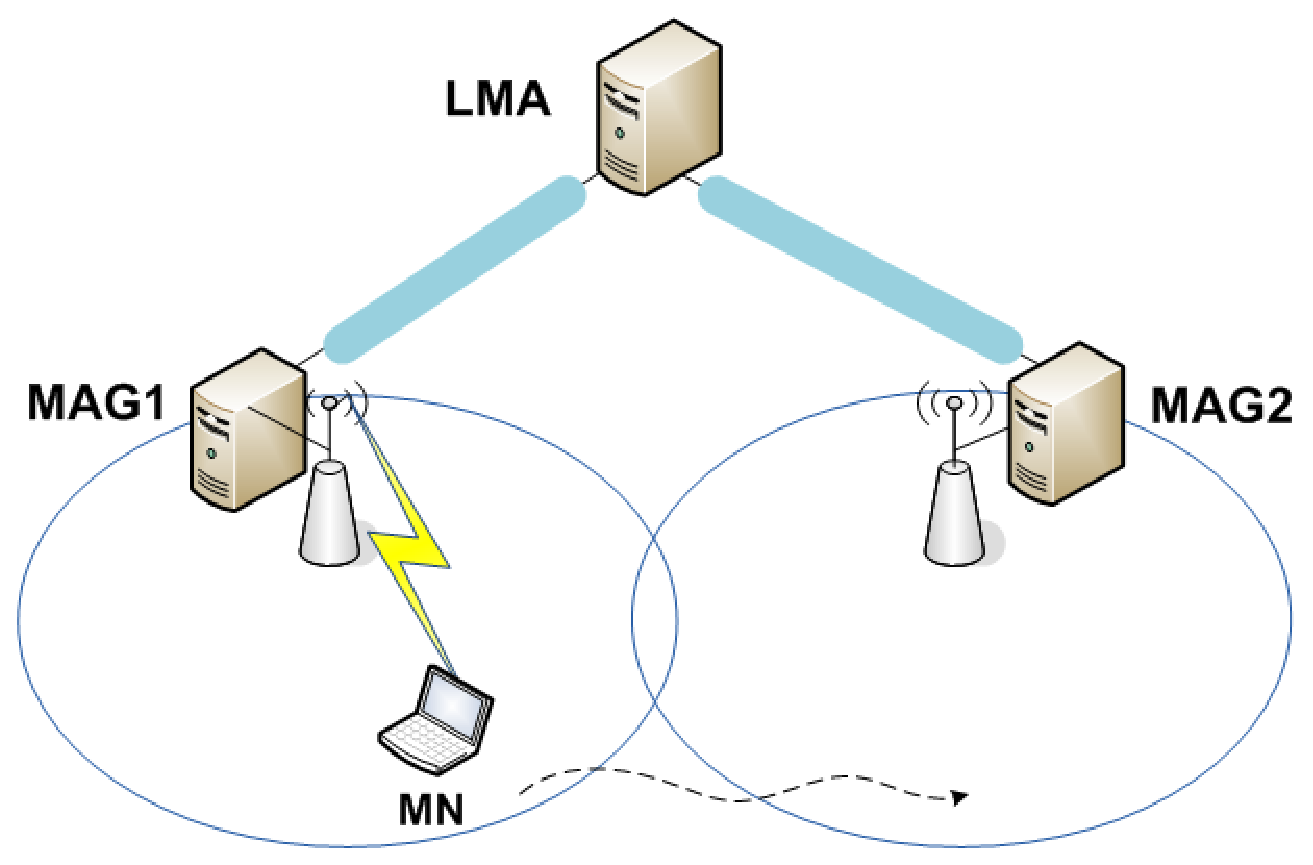
\includegraphics[width=0.50\textwidth]{./Part1/Chapter2/figures/c3_pmip_domain.eps} 
%    \caption[L'architecture d'un domaine PMIPv6]{L'achitecture d'un domaine PMIPv6.}
%     \label{fig:c3_pmip_domain}
%  \end{center} 
%\end{figure}
%
%Par rapport à MIPv6, PMIPv6 apporte certains avantages tels que: (i) évitant la complexité de la pile de protocole au MN; (ii) soutenant la mobilité sans la participation du MN; (iii) réduisant les surcharges de tunnel (sur l'air);  et (iv) diminuant la latence [73].
%
%L'opération de PMIPv6 est brièvement présentée comme suit : quand un MN entre dans un domaine PMIPv6 (attache à MAG1, par exemple), MAG1 va chercher le profil de MN (par exemple, à partir d'un serveur AAA). Puis deux messages de signalisation, le PBU et le PBA sont échangés entre MAG1 et LMA pour d'attribuer un (ou plusieurs) préfixe (s) (HNP) et mettre à jour l'emplacement actuel du MN. Un tunnel bidirectionnel est établi entre MAG1 et LMA pour rediriger le trafic de / vers le MN. Le MAG1 envoie alors un message RA, y compris l'HNP au MN. Le MN, basé sur l'HNP affecté, configure son adresse et peut l'utiliser pour communiquer avec un nœud correspondant (CN). Lorsque le MN effectue un handover de MAG1 à MAG2, le processus similaire sera exécuté pour mettre à jour l'emplacement actuel du MN au LMA. Le MAG2 obtient le même préfixe pour ce MN et peut émuler le réseau de la maison du MN (envoi des messages RA avec le même HNP). En conséquence, le MN n'est pas conscient de la mobilité et continue à utiliser la même adresse IP que précédemment.
%
%L'architecture actuelle de réseau mobile est très centralisée et hiérarchique. Ainsi les protocoles de mobilité IP (tels que PMIPv6 et DSMIPv6), qui ont été adoptés comme les protocoles de mobilité IP pour l'architecture EPC 3GPP, sont en ligne avec l'architecture centralisée et hiérarchique du réseau. Suite à l'architecture hiérarchique, les protocoles de gestion de la mobilité centralisée sont basés sur l'ancre de mobilité (HA dans MIPv6 et LMA dans PMIPv6) pour support à la mobilité. Par conséquent, à la fois le contexte de mobilité et l'encapsulation de trafic doivent être maintenus à l'ancre de mobilité. L'augmentation du nombre d'appareils mobiles et de leurs demande de trafic font des solutions de gestion de la mobilité centralisée à rencontrer plusieurs problèmes et limitations comme indiqué dans [9, 10]. Parmi eux, nous soulignons simplement les problèmes suivants :
%\begin{itemize}
%\item Le routage non optimal et le délai bout-à-bout : Lorsque le trafic de données traverse toujours l'ancre de mobilité centrale, il entraîne souvent une route plus longue. En particulier, lorsque le CN et le MN sont proches les uns des autres, mais loin de l'ancre. La même chose se produit dans le cas de CDN, dans lequel les fournisseurs de contenu mettent leurs données à la bordure du réseau. En conséquence, le délai de bout en bout sera augmenté.
%\item Le problème de l'évolutivité : La maintenance du contexte de MN et le traitement des paquets de / vers le MN nécessitent généralement des ressources de l'ancre de mobilité ainsi que les réseaux, donc réduisant l'évolutivité du système.
%\item Le gaspillage de ressources : Le service de la mobilité est toujours disponible même pour les sessions qui ne nécessitent pas le soutien de gestion de la mobilité. Ainsi, en apportant un soutien à la mobilité pour le MN/le service lorsque c'est vraiment nécessaire, les ressources de réseau peuvent être sauvées.
%\item La fiabilité: L'ancre de mobilité centrale en général constitue un goulot d'étranglement et point de défaillance unique.
%\end{itemize}
%
%La notion de DMM vise à répondre aux limites de l'approche de la mobilité centralisée soulevée quand un grand nombre d'appareils mobiles et le trafic de données sont pris en compte dans une architecture plate [9, 10]. DMM est actuellement un sujet brûlant, qui gagne beaucoup d'intérêt à la fois du monde universitaire et l'industrie. L'IETF a récemment affrété le groupe de travail DMM qui précise les solutions permettant de mettre en place des réseaux IP à l'appui d'un modèle d'ancrage distribué. Les concepts clés du DMM sont les suivants: i) les ancres de mobilité sont distribuées entre les entités de réseau et placées aussi près que possible du MN; et ii) la gestion de la mobilité est dynamique utilisée pour les sessions qui ont vraiment besoin de continuité de service. Dans DMM, une nouvelle entité est introduite - le MAR (Mobile Access Router). Cette entité peut jouer un rôle d'un HA, un LMA, un MAG ou un router normal.
%
%Dans l'approche basée sur le client, le MN est nécessaire pour participer au processus de signalisation. Chaque fois qu'un MN attache à un MAR, il obtient une adresse IPv6. Le MAR courant (cMAR) joue le rôle d'HA pour l'adresse attribuée à son réseau. Quand le MN attache au cMAR, il peut commencer une nouvelle communication avec le CN en utilisant l'adresse courante comme l'adresse de source du flux. Ce flux est acheminé de manière standard sans le mécanisme de tunnel. Lorsque le MN effectue un handover, si ce flux est encore en vie, il est acheminé via le routeur où ce flux a été initialement lancé (aMAR) en utilisant le mécanisme de tunnel entre le routeur et le MN. Pour ce faire, le MN doit mettre à jour son emplacement actuel à l'aMAR qui joue le rôle de son HA. Il est à noter que le MN doit effectuer une mise à jour de localisation pour chaque adresse IP active. En conséquence, il est nécessaire que le MN gère la liste d'HoA actifs et les aMARs associés, ainsi que la liste de sessions actives. En outre, le MN a besoin d'un mécanisme supplémentaire qui permet de sélectionner la bonne adresse IP à utiliser pour chaque session.
%
%Contrairement au DMM basé sur le client, l'approche basée sur le réseau ne nécessite pas le MN à participer au processus de signalisation. Le MAR effectue donc à la fois la fonctionnalité de LMA et de MAG. Agissant comme un MAG, le MAR détecte l'attachement du MN. Tout comme un LMA, il alloue une HNP au MN. Semblable au DMM basé sur le client, quand un MN attache à un MAR, il obtient une adresse IPv6. Typiquement, il peut utiliser l'adresse IP actuelle pour lancer des nouvelles sessions. Le trafic de données est acheminé en utilisant le routage IP normal sans aucun mécanisme de tunnelisation. Si le MN effectue un handover, le trafic sera acheminé à partir du MAR d'ancrage au MAR courant par le tunnel de la mobilité entre eux. Cependant, une question importante se pose est que la façon dont le cMAR apprend sur les adresses des aMARs. Il existe plusieurs mécanismes permettant le cMAR de connaître l'adresse des aMARs. La première méthode [90] repose sur une base de données centralisée (CMD) qui stocke les informations liées à la mobilité de chaque MN dans le domaine tel que la liste des HoAs, et l'adresse des aMARs associés comme similaire à [93]. Bien que cela permette de s'assurer que le processus de mobilité est totalement transparent pour le MN, ce mécanisme présente encore un point d'ancre centrale, cependant, pour le plan de contrôle seulement. La seconde méthode est basée sur l'information fournie par le MN comme spécifié dans [65]. En conséquence, le MN n'est plus transparent pour le processus de mobilité. Par conséquent, dans certains documents [69, 66], cette méthode est considérée comme un système basé sur le client comme indiqué ci-dessus.
%
%\subsection{Multicast IP dans le contexte de la mobilité}
%Afin de permettre le multicast IP dans MIPv6, deux approches de base ont été proposées, à savoir le tunnel bidirectionnel et la souscription à distance. Les deux approches ont leurs avantages et leurs inconvénients. Le tunnel bidirectionnel cache le déplacement des nœuds en acheminant le trafic multicast via le tunnel de mobilité entre le nœud et sa HA au prix de routage triangulaire (conduisant à un long délai) et le problème de la convergence du tunnel. D'autre part, dans l'approche de souscription à distance, le nœud multicast doit rejoindre les sessions en cours après chaque handover, ce qui pourrait mener l'interruption de service importante. En outre, des problèmes plus graves peuvent être augmentés en cas de mobilité de la source comme la transparence d'adresse et la maintien d'état de routage [11, 12]. Une amélioration supplémentaire devrait également être envisagée afin de satisfaire aux exigences supplémentaires en termes d'interruption de service et la perte de paquets pour les services en temps réel. Depuis tous ces protocoles sont conçus pour MIPv6 qui exigent les nœuds mobiles à participer au processus de signalisation, ils ne peuvent pas être appliqués directement à PMIPv6. Pourtant, l'idée de ces solutions peut être réutilisée.
%
%Comme les protocoles multicast sont conçus à l'origine pour un réseau fixe, considérant le multicast dans un environnement mobile apporte plusieurs défis au service multicast. La mobilité du nœud a des effets différents sur le service multicast, selon des facteurs tels que le rôle du nœud dans la session (source ou l'auditeur), le considéré modèle multicast (ASM ou SSM), le protocole de routage, le protocole de gestion du groupe et le protocole de mobilité en cours d'utilisation ainsi que la technologie d'accès sans fil. Par conséquent, les problèmes causé par la mobilité d'un nœud multicast peuvent être divisés en quatre groupes principaux : les problèmes généraux (en raison de protocoles multicast), les problèmes spécifiques de l'auditeur mobile, les problèmes spécifiques de la source mobile et les problèmes de déploiement [11, 12, 115]. Dans le cadre de cette thèse, nous nous concentrons sur les problèmes spécifiques de l'auditeur.
%
%La mobilité d'un auditeur provoque plusieurs problèmes pour le service multicast. Les problèmes et les solutions possibles sont décrits comme suit :
%\setlength \abovedisplayskip{-1pt}
%\vspace{-0.1in}
%\begin{itemize}
%\itemsep 0.07em
%\item L'interruption de service et la perte de paquets : Puisque le nœud mobile dans la gestion de la mobilité basée sur le réseau n'est pas au courant du processus de la mobilité, il ne peut pas prendre des décisions relatives au multicast, évitant un doux reprise de la session multicast. En conséquence, quand un auditeur se déplace à un nouveau MAG, il doit attendre pour exprimer son intérêt à s'abonner à des canaux multicast en cours jusqu'à ce qu'il reçoive une requête MLD. Ainsi, il éprouve un certain retard dans la réception de contenu multicast en raison du temps supplémentaire lié à l'activation du service multicast, la transmission MLD Query / Report (en particulier l'activation du service multicast qui est typique en quelques secondes). Ce problème devient plus grave lorsque les services en temps réel sont considérés.
%\item La duplication de paquets : Dans certains cas, le MAG peut recevoir le même paquet multicast à partir de différents LMAs ou MRs. Cela se produit lorsque différents tunnels MAG-LMA sont utilisés pour délivrer le trafic multicast.
%\item Le routage non optimal et le délai de bout en bout : Lorsque le trafic multicast doit passer par le point d'ancre de mobilité centrale (LMA), il entraîne souvent un plus long parcours. En conséquence, le délai de bout en bout sera augmenté. Ce problème devrait être prise en compte, en particulier lorsque les services en temps réel et les services sensibles au délai sont considérés.
%\item Le laisser de latence et le gaspillage des ressources de réseau : Puisque l'auditeur n'est pas conscient de la mobilité, il ne sera pas envoyer un rapport MLD pour quitter explicitement le groupe dans le MAG précédent (previous MAG - pMAG). En conséquence, si le dernier membre d'un groupe multicast se déplace à un autre MAG, le pMAG continuera d'offrir le trafic multicast jusqu'à ce qu'il met à jour ses informations des membres. Ainsi, il provoque une perte de ressources de réseau.
%\item En outre, l'auditeur peut recevoir le paquet hors de l'ordre en raison de handover. Dans de nombreux régimes sans fil, la signalisation liée au multicast doit être minimisée pour réduire la consommation d'énergie (avec la capacité limitée) et la ressource de réseau en cours d'utilisation. Encore une fois, l'ajustement des paramètres MLD [115] doit être soigneusement étudié comme un compromis des surcharges de signalisation et de l'interruption de service.
%\end{itemize}
%
%\paragraph{Les solutions en point de vue de l'IETF}
%
%Suite à une architecture typique de déploiement, le support multicast peut être activé en déployant le proxy MLD et la fonction de MR dans le domaine. En général, les différentes propositions sont issues en correspondant de l'emplacement de MAG et LMA dans l'architecture de déploiement de multicast. En conséquence, il existe deux approches principales correspondant aux différents rôles de MAG et LMA comme : i) MAG agit comme un proxy MLD tandis que LMA agit comme un MR ou un proxy supplémentaire; et ii) MAG et LMA jouent le rôle d'un MR. La première approche est considérée comme une solution de base par l'IETF. Cette solution peut également être considérée comme une solution basée sur le mécanisme de tunnelisation en raison du fait que le trafic multicast est routé via le tunnel de mobilité entre LMA et MAG. Dans la seconde approche, par le déploiement de routage multicast à MAG, plusieurs problèmes peuvent être évités (par exemple, le routage sous-optimal, problème de convergence) à un coût de fonctionnement et de déploiement du router multicast.
%
%\paragraph{La solution de base}
%La solution de base, qui a été normalisée par l'IETF, offre le soutien de la mobilité de l'auditeur dans PMIPv6 en plaçant la fonction proxy MLD au MAG, tandis que le LMA agissant comme un MR ou un proxy supplémentaire. La fonction proxy MLD est mise en œuvre au MAG avec l'interface « en amont » étant configuré vers le LMA. Comme une opération typique du proxy MLD, les données arrivant d'une interface « en amont » seront transmises aux interfaces « en aval » qui ont états appropriés pour ce groupe. Ainsi, tout le trafic multicast passe par le tunnel MAG-LMA, comme le trafic unicast. Après chaque handover, le trafic multicast continue de fournir à l'auditeur dans le nouveau MAG, et la continuité de service est assurée en conséquence. En outre, du point de vue de service multicast, l'auditeur ne connaît pas la mobilité. Il est atteint puisque le nouveau MAG, après l'obtention d'informations sur l'abonnement de l'auditeur en utilisant les opérations normales de MLD, rejoint les flux multicast courants de la part de l'auditeur. La solution de base peut être également appliquée à la source multicast [118].
%
%Lorsqu'un MN est attaché à un MAG (MAG1), après l'exécution des opérations PIMPv6 standards, MAG1 crée une instance proxy MLD (si nécessaire), qui sert comme un routeur « en amont » de tous les nœuds associés du LMA du MN. Cette instance ajoute le MN à son interface « en aval » et configure son interface « en amont » vers le LMA du MN. Lorsque le MN exprime sa volonté de recevoir le trafic multicast d'un groupe, il envoie un rapport MLD à MAG1. Le MAG1 envoie alors un rapport agrégé au LMA à rejoindre le groupe au nom du MN. Le LMA, agissant comme un MR, rejoint le groupe de l'infrastructure multicast, et met à jour son état de transmission. Après avoir reçu les paquets multicast, le LMA les transmet aux MAGs appropriées (via le tunnel LMA-MAG) en fonction de son état de transmission. Le MAG1 transmet ensuite les paquets aux interfaces appropriées « en aval » et ils ont finalement atteint le MN. En cas de handover (de MAG1 à MAG2), puisque la mobilité est transparente pour le MN, le MN ne sera pas envoyer les rapports MLD non sollicités. Au lieu de cela, MAG2, lors de la détection d'un nouveau MN sur la liaison d'accès, ajoute le MN à une interface « en aval », et envoie des messages MLD de requête générale sur sa liaison attachée. Le MN répond alors par un message MLD y compris les états actuels des groupes multicast. Sur cette base, MAG2 peut rejoindre les groupes au nom du MN. Les paquets multicast sont acheminés depuis LMA à MAG2 et atteignent finalement le MN.
%
%Bien que la solution de base soit un moyen très simple pour activer le support multicast dans PMIPv6, il ne traite pas des problèmes liés à la mobilité multicast. Dans plus de détails, l'utilisation de tunnel pour les flux multicast provoque la redondance du trafic (ou le problème de la convergence) au MAG. C'est parce que les différents nœuds, qui sont attachés au MAG et associés à différents LMAs peuvent s'abonner pour le même groupe. En outre, depuis plusieurs opérations doivent être exécutées pour permettre le MN continuer à recevoir le trafic multicast au nouveau MAG, il peut provoquer une longue interruption de service et un grand nombre de perte de paquets. En outre, comme le trafic multicast passe toujours par le LMA, il peut provoquer le problème de routage sous-optimal.
%
%\subsection{La mobilité d'un nœud multicast dans un domaine DMM orienté réseau}
%\begin{figure}[h!] 
% \begin{center} 
% 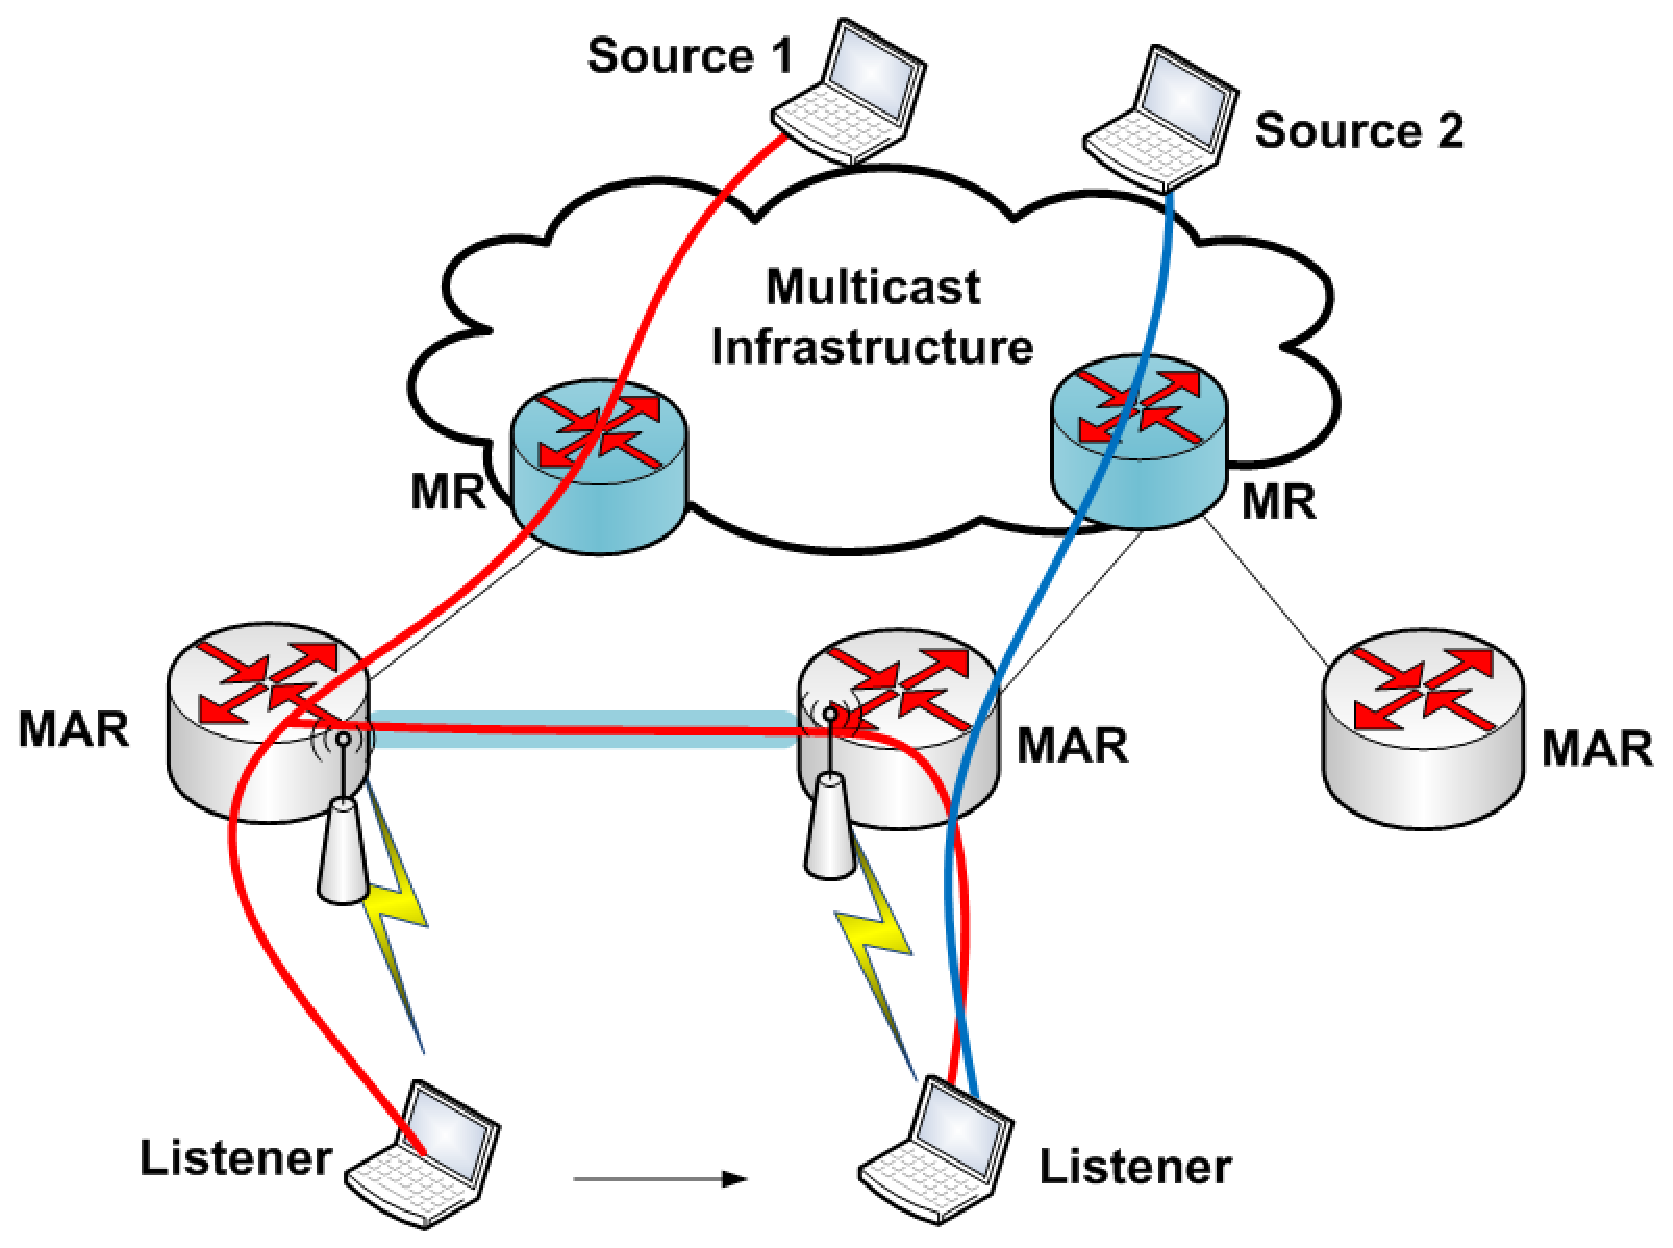
\includegraphics[width=0.50\textwidth]{./Part1/Chapter2/figures/c4_dmm_listener_mld.eps} 
%    \caption{La mobilité d'un auditeur dans un environnement DMM (la fonction de proxy MLD est déployée à MARs).}
%     \label{fig:c4_dmm_listener_mld}
%  \end{center} 
%\end{figure}
%
%Puisque DMM est encore à un stade précoce de la normalisation, il y a un travail limité pour le soutien au multicast. Jusqu'à présent, aucune solution complète n’a été trouvée pour le multicast dans DMM. En règle générale, tous les principaux aspects sont hérités du problème dans un domaine PMIPv6, tandis qu'une complexité supplémentaire est ajoutée. Il est à noter que cette section ne présente que les problèmes et les solutions en considérant un environnement DMM orienté réseau.
%
%Comme dans PMIPv6, le soutien à la mobilité de l'auditeur multicast peut être activé dans DMM en déployant le proxy MLD à MAR [128, 22, 20]. Dans ce cas, quand un flux multicast est lancé, le trafic multicast est reçu directement à partir de l'infrastructure multicast native via le MAR courant. Dans le cas du handover, le trafic est acheminé à partir de MAR d'ancrage au MAR courant via le tunnel entre eux (comme le trafic d'unicast). Cependant, ce mode ne traite pas des problèmes relatifs au multicast. Parmi eux, nous soulignons seulement les problèmes y compris l'interruption de service, le routage non-optimal, le délai de bout en bout, et le problème de la convergence, et la perte de paquets. 
%
%Considérant le déploiement de la fonction MR à MARs, le MAR décidera le trafic multicast d'un MR pour un auditeur attaché basé sur le Reverse Path Forwarding (RPF). Par conséquent, la convergence du tunnel et le routage non-optimal seront évités. Cependant, le mouvement de l'auditeur provoque le problème de l'interruption de service. En outre, les opérateurs ne veulent pas déployer la fonction de routage multicast sur le MAR en raison de sa mise en œuvre et le coût d'exploitation par rapport à proxy MLD.
%
%\subsection{Evaluation de la performance}
%\subsubsection{Métriques pour l'évaluation de la performance}
%Pour évaluer la performance d'un protocole de gestion de la mobilité, un ensemble de paramètres est en général considéré incluant le coût de signalisation, le temps de handover (temps de latence), le délai de bout en bout et le coût de tunnelisation. Le coût de signalisation est défini comme le coût de mettre à jour l'emplacement du MN. Il est un facteur important car il influence l'évolutivité du système ainsi que le coût de livraison de données, en particulier lorsqu'on considère environnement sans fil qui a typiquement une capacité limitée. En ce qui concerne le temps de latence, il est définie comme une période où un nœud ne peut pas recevoir / envoyer des paquets en effectuant un handover. C'est le temps écoulé entre le dernier paquet reçu via l'ancien routeur et l'arrivée du premier paquet via le nouveau routeur après un handover. Au cours de cette période, les paquets sont perdus. Ainsi, il peut entraîner de l'interruption notable de service, surtout dans le cas d'applications sensibles au délai comme la vidéo et la voix sur IP (VoIP). Le nombre de paquets perdus est généralement proportionnel à la latence de handover. Dans les réseaux basés sur IPv6, QoS peut être définie par la perte de paquets, la latence et les surcharges de signalisation [72]. En conséquence, une longue période de latence et un grand nombre de paquets perdus peuvent dégrader la qualité du service. Par conséquent, la réduction du temps de latence et de la perte de paquets améliore la performance de l'application. D'autre part, le délai de bout en bout entre deux nœuds est la somme des retards rencontrés au long du trajet entre ces nœuds. En général, le délai de bout-en-bout comprend non seulement le délai de la transmission sur les liens, mais également la mise en attente de traitement et de retard au niveau des nœuds intermédiaires [133]. Des nombreuses applications populaires de multimédia (par exemple, le jeu en temps réel, le streaming vidéo en direct et VoIP / Vidéo conversationnel) ont de délai strict.
%\begin{figure}[h!] 
% \begin{center} 
% 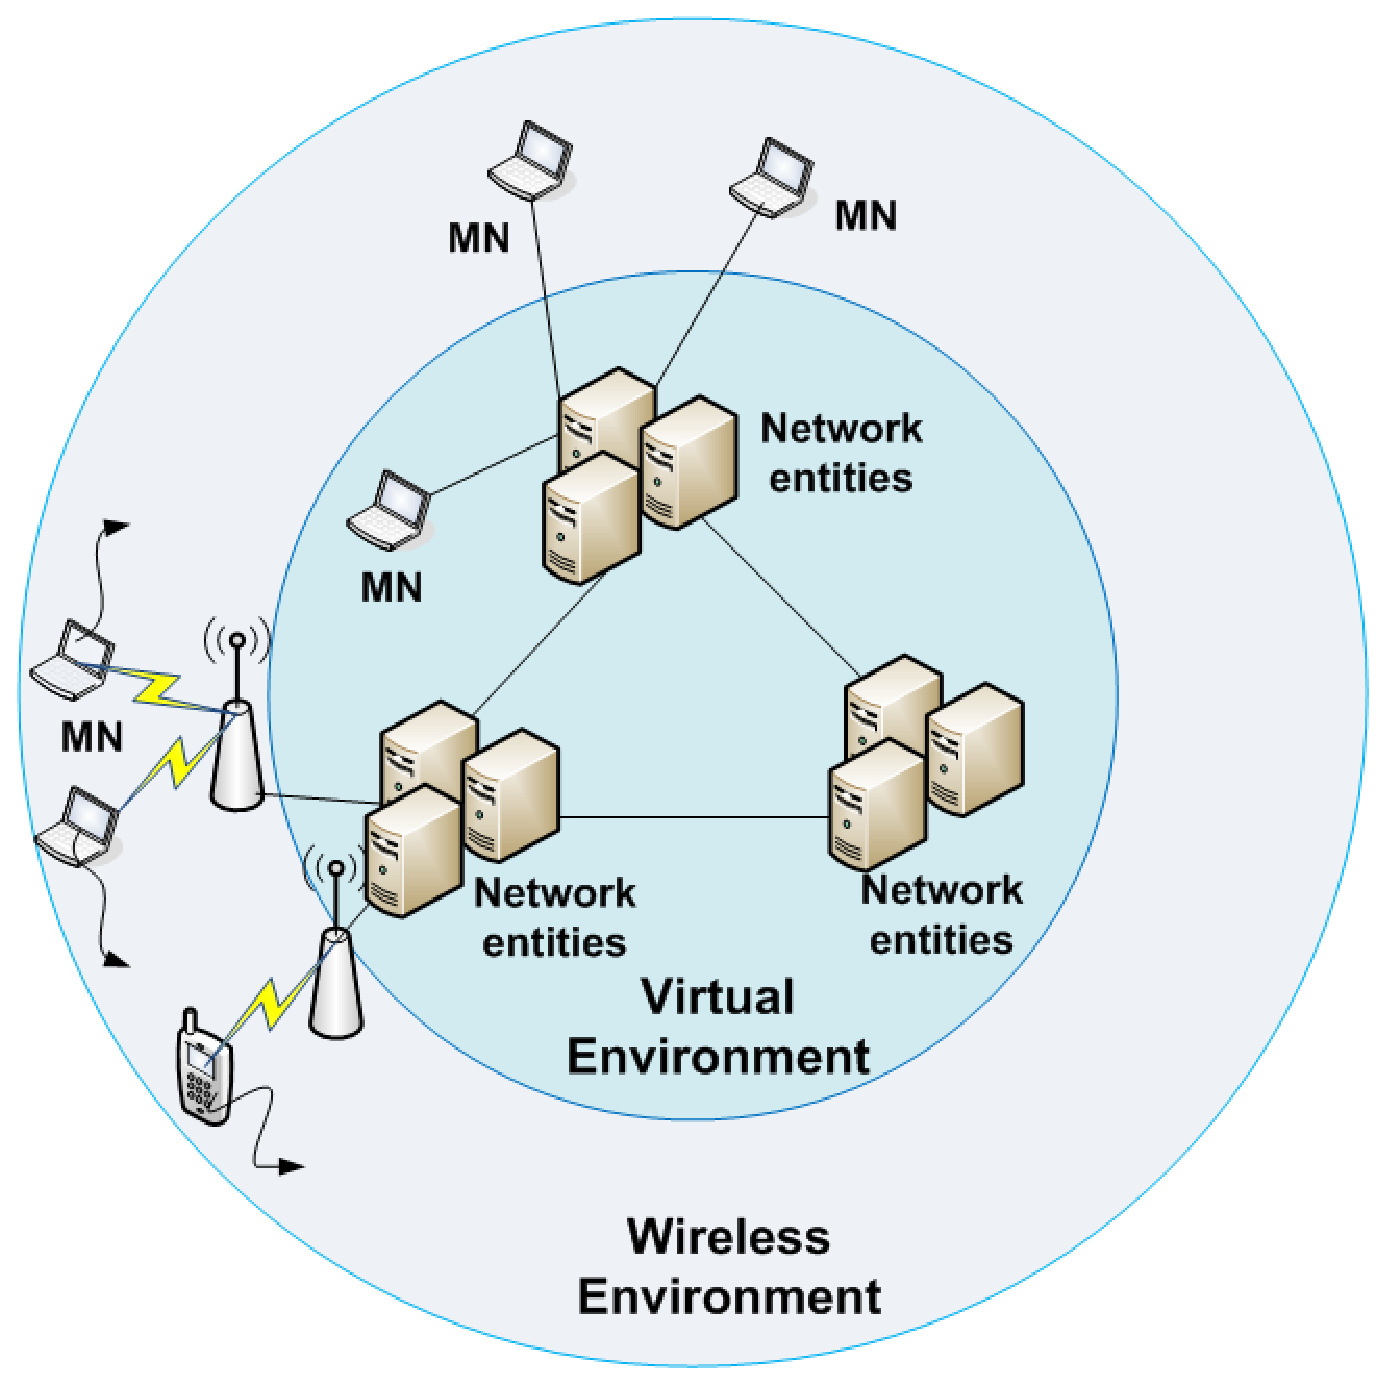
\includegraphics[width=0.45\textwidth]{./Part1/Chapter3/figures/c5_architecture.eps} 
%    \caption{L'architecture d'un banc d'essai proche de réel.}
%     \label{fig:c5_architecture}
%  \end{center} 
%\end{figure}
%
%\subsubsection{Evaluation expérimentale pour les réseaux sans fil}
%Dans la recherche en réseau, il y a des diverses méthodes d'expérimentation, tels que : le banc d'essai réel, la simulation, l'émulation, la virtualisation et la modélisation mathématique (ou théorique). Chaque méthode a ses avantages et ses limites [135]. L'utilisation d'un banc d'essai réel est considérée comme la meilleure méthode expérimentale. Cependant, elle implique un coût plus élevé de déploiement et manque d'évolutivité. Bien que la simulation soit très populaire grâce à sa flexibilité et facile à déployer des fonctionnalités, les résultats obtenus dans certains cas, ne sont pas fiables. L'émulation peut être considérée comme un compromis entre la simulation et un banc d'essai réel apportant des résultats plus précis (par rapport à la simulation) et à moindre coût (par rapport au banc d'essai réel). Pourtant, l'émulation a des limites sur le déploiement et l'évolutivité, qui peuvent être atténués en utilisant la technique de virtualisation. Enfin, la modélisation mathématique est parfois utilisée, mais seulement d'une façon simplifiée, en faisant abstraction de la complexité. En outre, pour aider à justifier notre approche sur la méthode expérimentale, nous devons mentionner que notre étude concerne les environnements mobiles et nous devons donc garder à l'esprit les exigences les plus importantes que d'une méthode expérimentale doit se concentrer sur sont la précision, la fiabilité, la mobilité et l'évolutivité [136 ].
%
%Dans cette thèse, nous introduisons un environnement d'expérimentation proche du réel qui se compose d'un environnement de virtualisation et simulation. La première partie peut être considérée comme l'infrastructure du réseau dans lequel les multiples machines virtuelles sont reliées, tandis que la seconde partie est un réseau d'accès sans fil essentiellement composé par le simulateur NS-3. En combinant ces éléments, nous avons produit une méthode qui peut atteindre un niveau supérieur de réalisme en conservant les avantages de la méthode de simulation et encore être en mesure d'exécuter des logiciels et des protocoles réels. Puisque cet environnement est un open-source et facile à déployer, il peut être réutilisé par d'autres chercheurs à créer leur propre environnement d'expérimentation. De plus, il permet la conception et l'évaluation du réseau de taille petit à moyenne et de déployer les protocoles dont les résultats peuvent être facilement convertis dans le monde réel. En particulier, cette méthode est appropriée pour les cas suivants : i) l'infrastructure fixe; ii) la mobilité et les réseaux mobiles; iii) l'expérimentation de la couche supérieure à la couche réseau (par exemple, la gestion de la mobilité, le multicast, les applications, etc.); iv)  l'infrastructure du réseau de taille moyenne; et v) le réseau de taille grande en fonction de nœuds mobiles.
%
%\vspace{-0.22in}
%\section{La mobilité d'un nœud multicast dans PMIPv6}
%\subsection{Optimisation de la continuité de service dans un domaine PMIPv6}
%
%La solution de base a été récemment adoptée pour soutenir la mobilité de l'auditeur dans PMIPv6. Néanmoins, elle ne traite pas des problèmes d'optimisation et de performance tels que le temps d'interruption de service, les surcharges de tunnel, et le routage non optimal, etc. En ce qui concerne le temps d'interruption de service, nous proposons une méthode basée sur la combinaison des mécanismes de transfert de contexte multicast et de fonction de suivi explicite pour minimiser le temps d'interruption. Commençant par l'analyse du temps de l'interruption, les expériences sont ensuite effectués pour comparer différentes approches reposant sur un banc d'essai près au réel. Les résultats numériques et expérimentaux montrent que grâce à l'utilisation de transfert de contexte multicast, le temps d'interruption peut être réduit de manière significative. En ajustant le comportement du MLD pour les routeurs, nous pouvons également obtenir un résultat similaire, mais arrive une dramatique augmentation de la signalisation liée au multicast. Particulièrement, le problème sera plus grave avec un grand nombre d'auditeurs. En outre, grâce au transfert de contexte multicast le temps de congés (leave latency) est minimisé. Par conséquent, le protocole de transfert de contexte en général peut être considéré dans les solutions proposées. A noter que la fonction de transfert de contexte et la fonction de suivi explicite mises en œuvre peuvent être utilisées dans notre banc d'essai, ainsi que dans un vrai banc d'essai. Notre banc d'essai peut être servi comme un banc d'essai proche du réel, qui peut fournir des résultats réalistes à faible coût pour l'expérimentation de la mobilité multicast dans un domaine PMIPv6.
%\begin{figure}[h!] 
% \begin{center} 
% 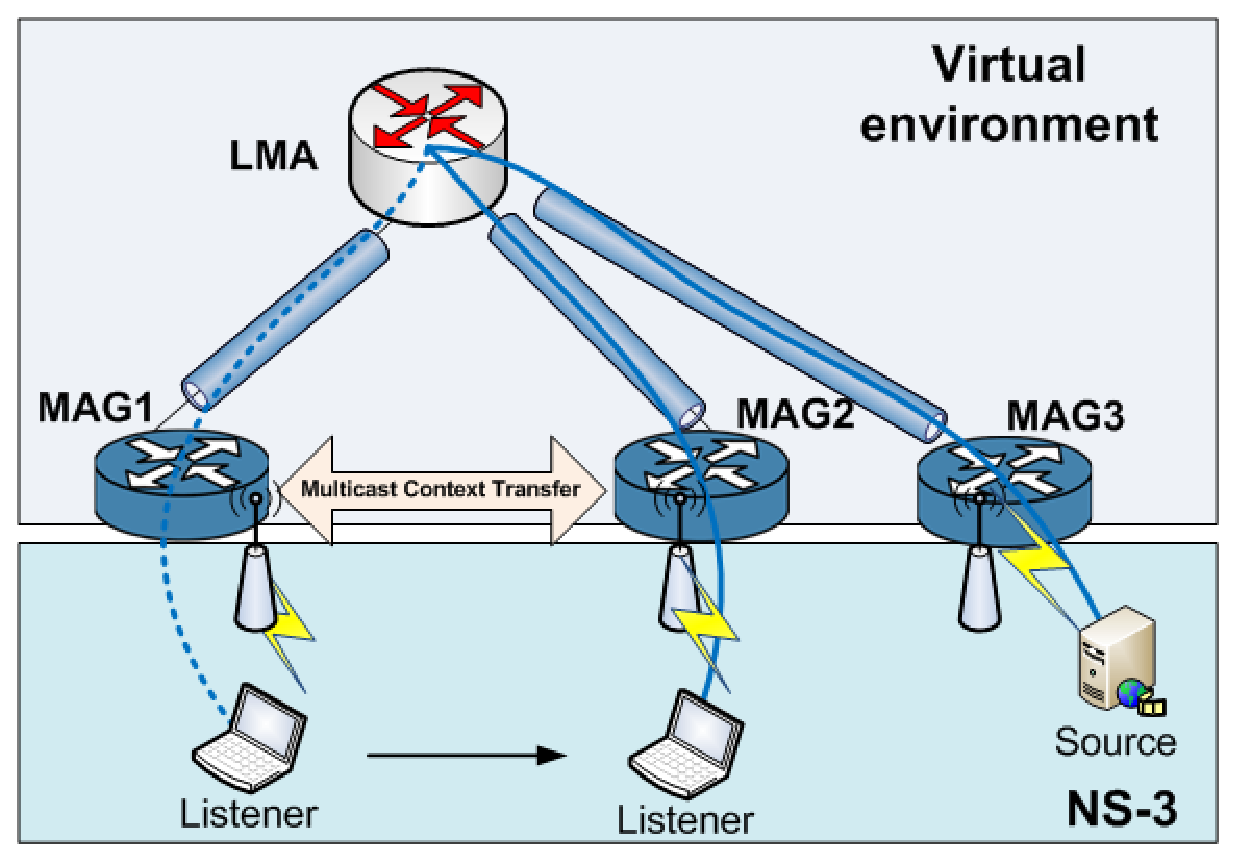
\includegraphics[width=0.53\textwidth]{./Part2/Chapter4/figures/optimizing.eps} 
%    \caption{Le déploiement d'un banc d'essai proche au réel.}
%     \label{fig:c5_architecture}
%  \end{center} 
%\end{figure}
%
%Pour réduire le temps d'interruption, l'objectif est de réduire le temps nécessaire au nouveau MAG (nMAG) pour obtenir des informations d'abonnement multicast actives du MN pendant handover. Alors que le nMAG peut s'abonner à des flux courants (à l'avance) et transmet les paquets multicast au MN dès que possible. Pour ce faire, des informations  d'abonnement sont échangées entre le pMAG et le nMAG. En outre, cette solution est indépendante de la technologie de la couche 2 et plus facile à déployer que les propositions existantes. Le transfert de contexte multicast est également mis au point conformément à la norme pour le protocole de transfert de contexte [159]. En outre, la solution proposée ne met pas de charge supplémentaire sur le LMA, ce qui rend notre solution meilleure en comparaison avec la solution M-LMA en termes d'évolutivité.
%
%\subsection{Equilibrage de charge du flux multicast dans les réseaux PMIPv6 }
%La croissante de la pénétration des appareils mobiles, tels que les tablettes et les téléphones intelligents génère un grand nombre de trafic de données, en particulier le trafic vidéo sur les réseaux mobiles [6, 1]. Dans ce contexte, il est fréquent d'avoir un grand nombre de périphériques associés au LMA dans un domaine PMIPv6 donc facilement faire le LMA un goulot d'étranglement et un point de défaillance unique. Par conséquent, la qualité des sessions en cours pourrait être dégradée (par exemple, une augmentation du délai de la file d'attente et une augmentation du perte de paquets). En conséquence, les opérateurs des réseaux mobiles peuvent avoir besoin de déployer plusieurs LMAs dans un grand domaine PMIPv6, de sorte que le trafic peut être réparti entre les LMAs [76]. Pourtant, il est fort possible que certains LMAs deviennent surchargés alors que les autres sont sous-utilisés. Par conséquent, l'équilibrage de charge (LB) entre les LMAs est nécessaire. Du fait que le multicast IP devrait être largement déployé dans un proche avenir pour faire face à une énorme demande de trafic multimédia. Ainsi que, le contenu de la vidéo mobile a généralement des débits beaucoup plus élevés que les autres types de contenu. Le service multicast devrait donc jouer un facteur crucial dans la mise charge sur le LMA. Cependant, son rôle a été négligé dans toutes les propositions existantes. Par conséquent, l'utilisation de service multicast dans les mécanismes LB existants peut conduire à plusieurs problèmes à la fois de LB (la dégradation de l'efficacité) et de service multicast (par exemple, le problème de la convergence et  l'interruption de service).
%
%Pour ces raisons, nous introduisons un mécanisme d'équilibrage de charge (en fonction de multicast), qui prend le service multicast en compte. L'idée clé est que par la séparation du mécanisme d'équilibrage de charge multicast à partir de l'unicast, la solution proposée permet de mieux répartir la charge entre les LMAs dans runtime, ainsi que d'améliorer l'efficacité de l'utilisation des ressources.
%
%Dans plus de détails, deux approches différentes, à savoir l'approche proactive multicast (ou MAG-initié) et  l'approche réactive multicast (ou LMA-initié) sont considérées. Dans le premier cas, le mécanisme LB sera appelé lorsqu'un MN démarre une nouvelle session multicast pour sélectionner un LMA approprié à servir cette session. Dans ce dernier cas, le mécanisme LB sera exécuté quand un LMA est surchargé en sélectionnant une session de multicast pour passer à un LMA moins chargée. Il peut être fait grâce à une extension de proxy MLD pour supporter de multiples interfaces « en amont » [167]. Dans ce cas, une seule instance de proxy est déployée à MAG avec plusieurs interfaces « en amont » étant configurées vers différents LMAs. En conséquence, le MN peut recevoir le trafic multicast à partir d'un LMA moins chargé, en obtenant le trafic unicast à partir de sa LMA. Par conséquent, la solution proposée ne modifie pas les sessions multicast/unicast en cours.
%
%\subsection{Mobilité dans les réseaux hétérogènes}
%La mobilité dans les réseaux hétérogènes sera illustrée via un cas d'utilisations: le service de recharge de véhicule électrique (EVCS). Il y a plusieurs raisons pour choisir ce cas d'utilisation. Tout d'abord, le véhicule électrique (EV) est un choix prometteur pour le transport personnel dans un proche avenir. Deuxièmement, l'idée de connexion des véhicules prend de l'ampleur. En outre, un nœud mobile (ou un véhicule électrique dans ce contexte) peut être relié à l'infrastructure via différentes technologies sans fil / filaires dans différentes étapes. Ainsi, compte tenu multicast dans le véhicule électrique est une étape pour permettre de déployer système de divertissement à l'EV, qui devient de plus en plus populaire. En outre, le multicast IP peut également être utilisé pour mettre à jour le logiciel des systèmes embarqués.
%
%\begin{figure}[h!] 
% \begin{center} 
% \includegraphics[width=0.80\textwidth]{./Part2/Chapter6/figures/c8_use_cases.eps} 
%    \caption{Les cas d'utilisation de service EVCS.}
%     \label{fig:c5_architecture}
%  \end{center} 
%\end{figure}
%
%Comme indiqué dans [184], la condition essentielle pour obtenir des avantages énergétiques et économiques de Smart-Grid et de véhicules électriques est d'atteindre un ordonnancement optimal de la charge des véhicules électriques et le stockage de l'électricité par les EVs. Ainsi, il est important pour les opérateurs du Grid de surveiller les données nécessaires (comme la consommation d'énergie et la demande) et d'attribuer et de router des véhicules vers les stations de recharge appropriées pour appuyer leurs politiques de tarification nécessaires. Cette négociation ne peut être menée à la station de charge, mais doit être effectuée pendant la conduite. L'EV doit donc communiquer avec l'infrastructure de charge [185]. Dans ce contexte, plusieurs technologies d'accès (par exemple, WLAN, LTE, et PLC) doivent être utilisés lors des différentes phases de l'EVCS, comme LTE pendant la conduite, WLAN en approchant une station de charge, et PLC en étant amarré à une station de recharge. Ces technologies de communications hétérogènes doivent être transparentes pour l'utilisateur, la gestion de réseau et pour l'EVCS afin de maintenir le contexte de service.
%
%Nous vous proposons une solution de EVCS à la fois point de vue de l'utilisateur et de l'opérateur de Grid. Pour l'utilisateur, il offre un service omniprésent et  transparent à différents scénarios (à la maison, à une station de charge et à un parking), ce qui rend le chargement d'un EV aussi simple que possible. Il contribue également à l'operateur du réseau de gérer efficacement la consommation de l'utilisateur et la demande sur le Grid, surtout quand un grand nombre de véhicules électriques est considéré. De la nature centralisée de service de Smart-Grid, une solution de la gestion de la mobilité centralisée basée sur le réseau, par exemple, PMIPv6 est le plus appropriée pour fédérer les services de charge segmentés et faire l'expérience de charge transparente de la mobilité des EVs ainsi que la technologie de communication utilisée par chaque phase du EVCS. En utilisant PMIPv6, le service prend en charge la mobilité des EVs, les handovers verticaux et horizontaux entre les différentes technologies de communication. Pourtant, la conservation de l'adresse IPv6 dans PMIPv6 reste un problème dans un tel contexte, et nous fournissons une solution en s'appuyant sur une approche de l'interface logique pour cacher la modification de l'interface vers la pile IPv6 (du point de vue de la couche IP). Le concept d'EVCS et la performance du PMIPv6 pour l'EVCS ont été validés à l'encontre de référence de la norme IEEE 1646. Un banc d'essai proche au réel, qui est une combinaison des machines réelles et virtuelles, a été déployé pour réduire le coût du matériel et de fournir d'expérience flexible. Un lien réel PLC fournis par les partenaires du projet VELCRI est utilisé pour obtenir des résultats réalistes.
%
%\subsection{La mobilité inter-domaine : du point de vue du DMM}
%Comme mentionné précédemment, en profitant de la gestion de la mobilité basée sur le réseau, PMIPv6 permet à la mobilité IP pour déplacer les clients sans leur participation. PMIPv6 apporte plusieurs avantages par rapport à la gestion de la mobilité basée sur le client comme MIPv6. Cependant, PMIPv6 échoue à soutenir la mobilité inter-domaine. Cela signifie que, même si un MN se déplace vers un autre domaine PMIPv6, la continuité de la session ne peut être maintenue.
%
%Afin de soutenir la mobilité inter-domaine, plusieurs solutions ont été proposées, par exemple, l'intégration de MIPv6 et  PMIPv6 (H-PMIP) [192]; et  I-PMIP [193]. Pourtant, elles ont des limitations telles que le routage sous-optimal, les surcharges de signalisation et la latence de handover. Surtout, en raison du manque de granularité sur le service de gestion de la mobilité, la mobilité est toujours disponible même pour les sessions qui ne nécessitent pas de support de gestion de la mobilité (par exemple, les sessions qui sont lancées et terminées alors que le nœud mobile connecté au même domaine).
%
%Basé sur le concept DMM, nous introduisons un support à la mobilité inter-domaine, appelé D-PMIP. Ainsi, cette proposition apporte certains avantages : (i) les ancres de mobilité sont placées près de MN; et  (ii) le service de la mobilité n'est disponible que pour les sessions qui nécessitent vraiment la continuité du service. Une fois que le MN entre son domaine PMIPv6, il obtient un préfixe. Basé sur le préfixe attribué, le MN configure son adresse IPv6. Le MN peut ensuite utiliser cette adresse pour initier et maintenir les sessions de façon standard alors qu'il reste attaché à ce domaine. Lorsque le MN change son domaine, il obtient un autre préfixe et configure une nouvelle adresse basée sur ce préfixe. Cette adresse peut être utilisée pour mettre en place les nouvelles sessions. Jusqu'à ce que les sessions précédentes ne soient pas fermées, les anciennes adresses doivent être maintenues. Ainsi, un tunnel est construit entre le LMA d'ancrage et le LMA actuel à rediriger les paquets entre deux LMAs.
%
%Basé sur le concept DMM, deux solutions possibles pour la mobilité inter-domaine sont considérées, à savoir la solution de partie distribuée (DP-PMIP) et la solution d'entier distribuée (DF-PMIP). La première solution repose sur une base de données commune pour le plan de contrôle, alors que dans la dernière la fonction de la mobilité est répartie dans les deux plans : le plan de contrôle et le plan de données. Ainsi, deux solutions permettent à des paquets de données à être acheminés via une manière quasi-optimale en mettant les points d'ancrage de mobilité plus proche du MN tandis que le plan de contrôle peut être placé n'importe où dans le réseau. Les résultats numériques montrent que la solution DP-PMIP donne des meilleures performances que les solutions existantes (par exemple, MIPv6, H-PMIP et I-PMIP) en termes de latence, de coût de signalisation et d'utilisation du tunnel.
%\section{La mobilité d'un nœud multicast dans DMM}
%
%Comme indiqué précédemment, le multicast IP peut être activé dans DMM en déployant la fonction proxy MLD à MAR. Pour le nouveau flux, le trafic multicast est transmis directement à partir de l'infrastructure multicast via le MAR courant. Pour le flux après le handover, le trafic est tunnelé du MAR où le flux est initié au MAR courant par le tunnel de la mobilité entre eux. Ainsi, le point d'ancre de mobilité multicast (MMA) est associé à la phase initiale du flux multicast (identique à l'ancre de mobilité unicast) : le MAR où le flux est initiée. Le flux multicast sera ancré au MMA initialement attribué au cours de sa vie. Par conséquent, même lorsque le MN se déplace loin de son point d'ancre, le trafic de multicast traverse encore l'ancre. En conséquence, il provoque plusieurs problèmes au flux multicast en cours, comme l'interruption de service, le routage non-optimal, le délai de bout-en-bout et la duplication de paquets. Ces problèmes deviennent graves lorsqu'on considère les services sensibles à l'interruption et aux délais. En outre, même les ancres de mobilité sont distribuées, des ancres sont plus surchargées que les autres \cite {anchor_selection}.
%
%Dans cette section, nous soutenons principalement la nécessité d'un mécanisme de sélection dynamique de l'ancre de mobilité multicast (DMMA). D'un point de vue du service, il contribue à satisfaire les exigences en termes de l'interruption du service et le délai, en particulier lorsqu'on considère les services en temps réel. Il fournit un mécanisme permettant de mieux répartir la charge entre MARs. En outre, d'autres problèmes telles que la duplication de paquets et le laisser latence (perte de ressources) peuvent être réduits. Le DMMA prend en compte non seulement le contexte du service, mais aussi le contexte de la mobilité du nœud et le contexte du réseau, permettant un support par flux. En d'autres termes, chaque flux multicast peut être traité différemment selon différents contextes.
%
%\subsection{La mobilité de l'auditeur dans DMM} \label{c10:multicast_listener}
%
%En ce qui concerne l'interruption de service, quand un auditeur multicast se déplace de pMAR à cMAR, il peut provoquer une interruption de service perceptible pour les flux en cours. En conséquence, le transfert de contexte multicast est nécessaire pour éviter une grande interruption causée par les procédures relatives au service multicast (environ 5 s dans le cas normal, et de 2,5 s dans le meilleur des cas) \cite{Thinh_WCNC_Multicast}. Ce délai est beaucoup plus long que le temps d'interruption de tolérance maximum pour les services normaux, comme spécifié dans \cite{interruption_requirements} est de 500 ms. Même avec le transfert de contexte, il est incapable de répondre à l'exigence en termes d'interruption pour le service sensible à l'interruption lorsque le délai cMAR-aMAR est grand \cite{Thinh_ICNS,multicast_DMM_Sergio_PIMRC}. C'est parce que le trafic multicast doit passer par l'aMAR, qui joue le rôle de point d'ancrage de multicast (MMA). En outre, puisque le trafic de multicast traverse toujours l'aMAR, il entraîne souvent une route plus longue. Particulièrement, considérant un grand domaine, il peut provoquer un délai de bout en bout élevé. Ce problème devient plus sérieux lorsque le service sensible au délai est considéré.
%
%
%En cas de mobilité, l'utilisation du tunnel pour le flux multicast peut entraîner le problème de la convergence. Puisque le but de DMM est de déplacer les ancres de mobilité du coeur vers la périphérie du réseau, le nombre de points d'ancrage dans un domaine DMM sera beaucoup plus que celui dans un domaine PMIPv6. En conséquence, le problème de la convergence est supposé être bien plus sévère que celui dans PMIPv6. En utilisant une extension de proxy MLD pour supporter de multiples interfaces « en amont » \cite{multiple_upstreams}, le problème de la convergence peut être évité. 
%
%\begin{figure}[tb!] 
%  \begin{center} 
%    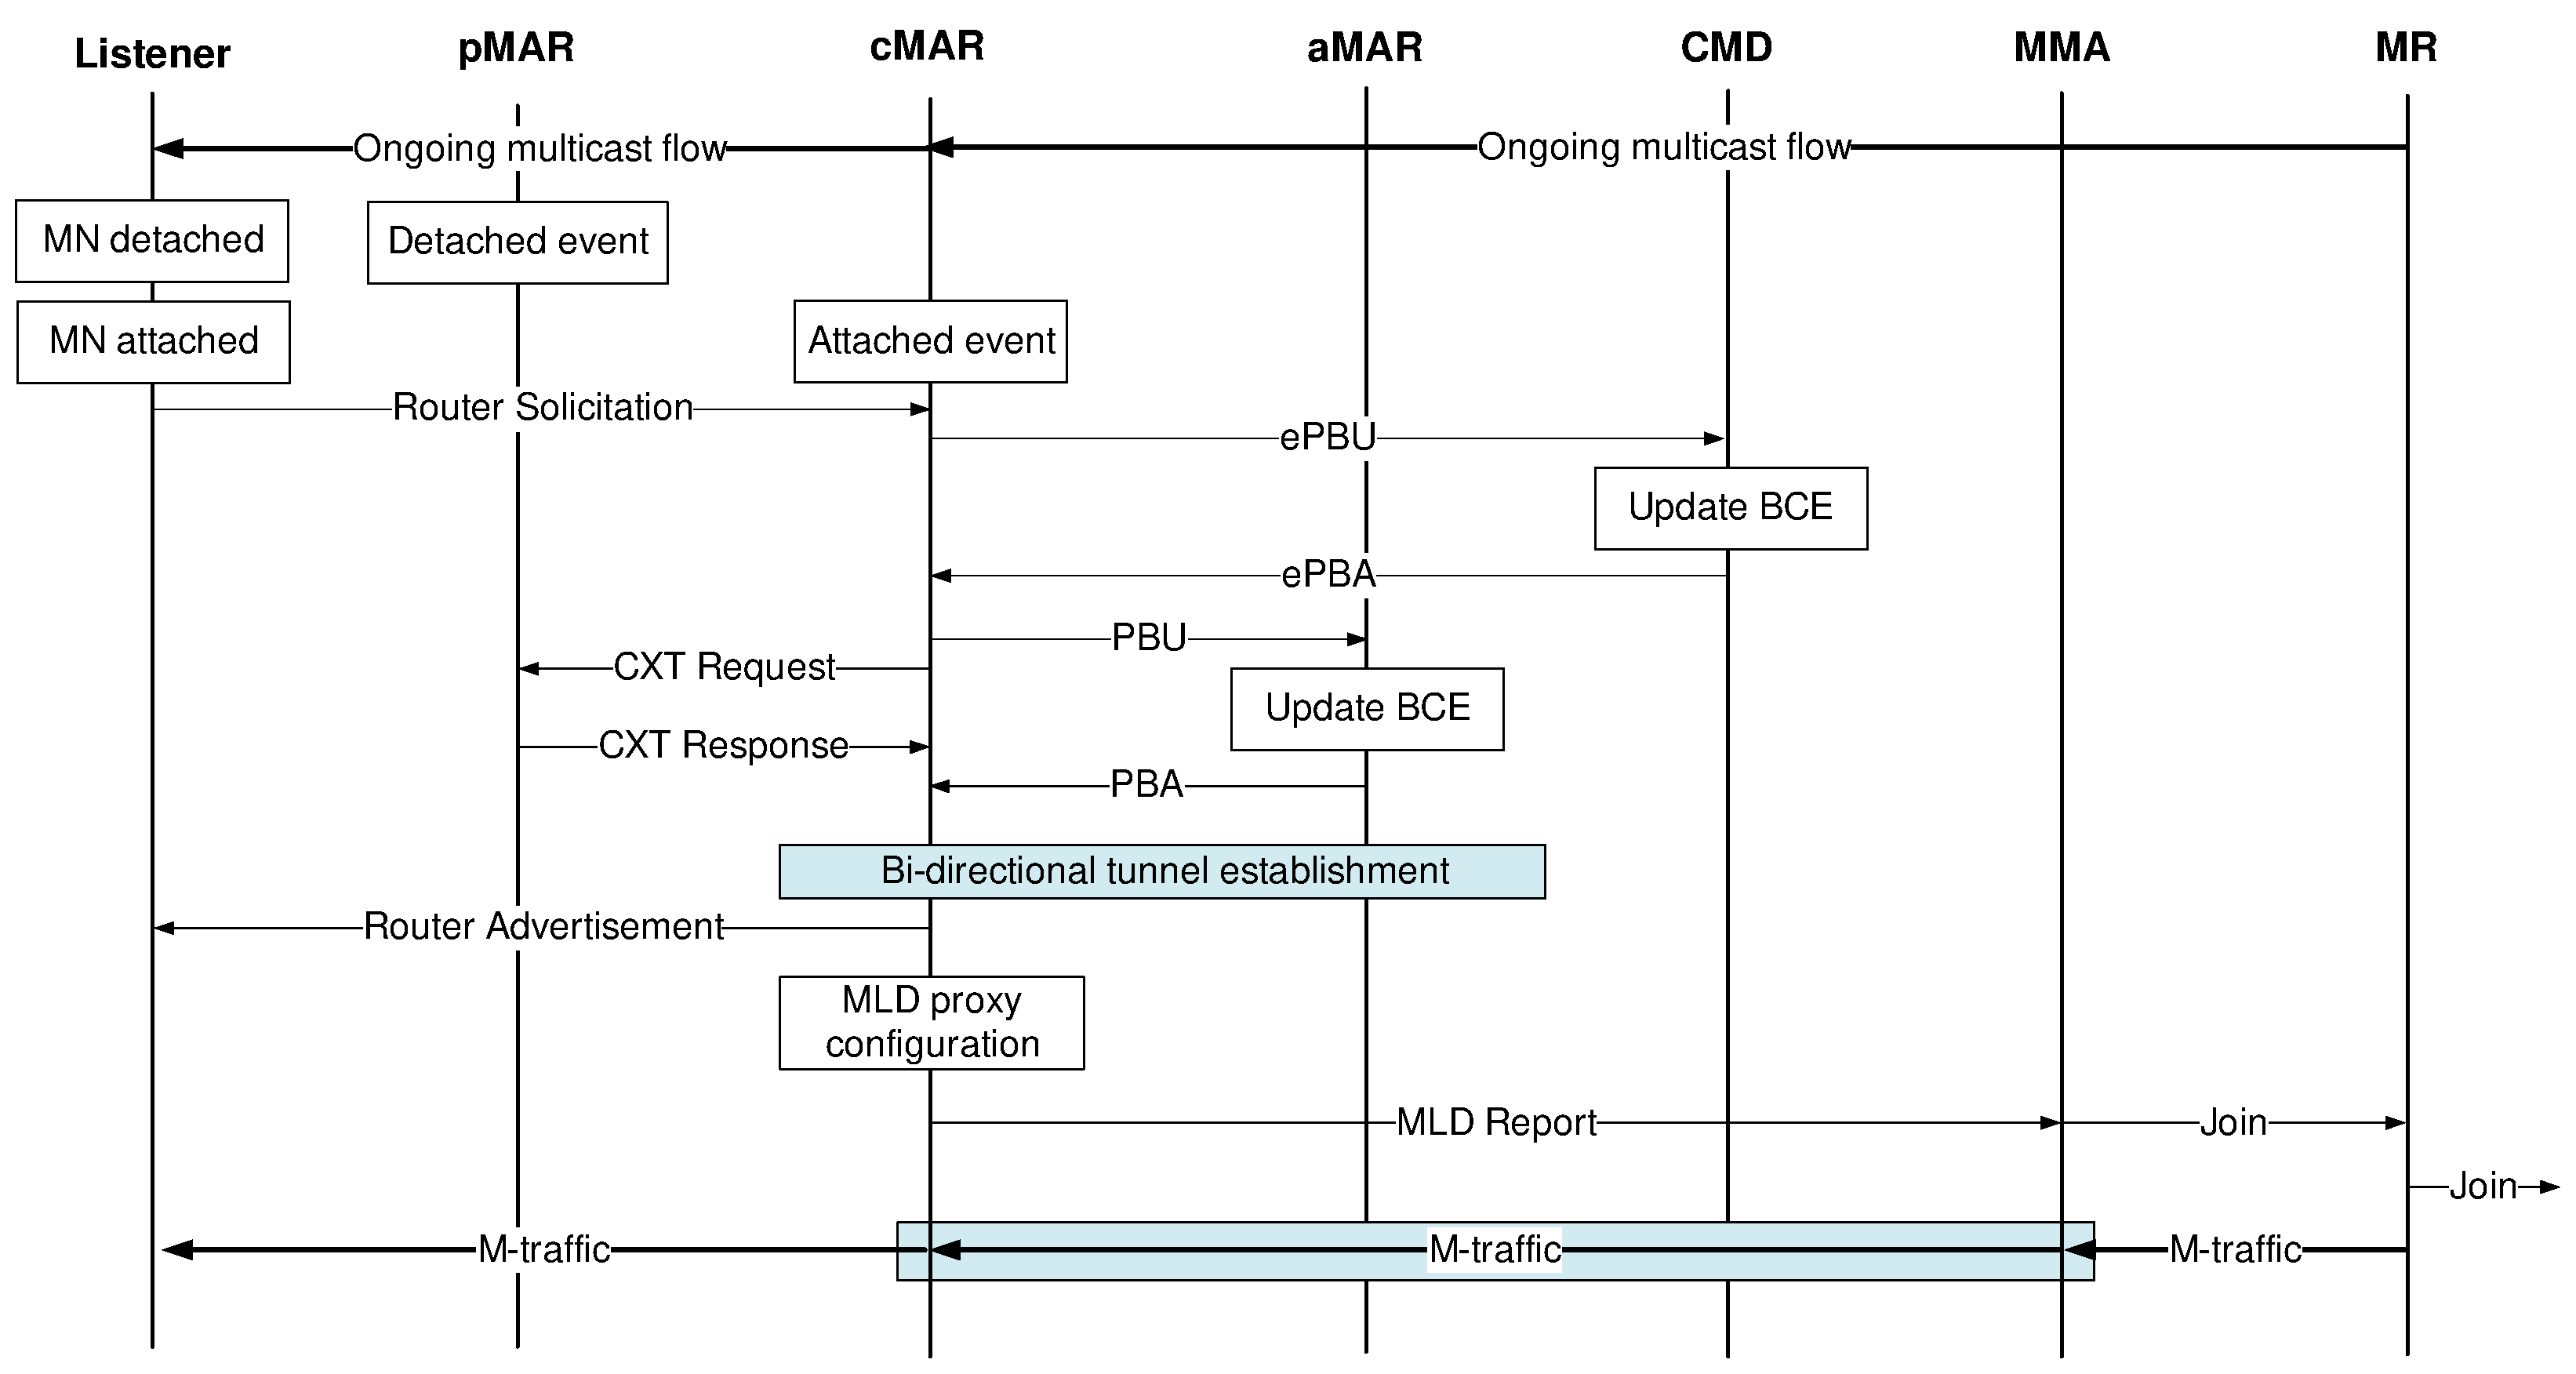
\includegraphics[width=0.90\textwidth]{./Part3/Chapter8/figures/c10_service_disruption_common.eps} 
%    \caption[La signalisation quand un auditeur exécute un handover.]{La signalisation quand un auditeur exécute un handover.}
%    \label{fig:c10_HO}
%  \end{center} 
%\end{figure}
%
%Pour souligner ces problèmes, nous considérons différents candidats pour le MMA comme l'aMAR (le mode par défaut), le pMAR, le cMAR (le subscription native), ou un MMA commun (COMMA) qui sert comme un seul MMA pour le domaine (comme dans \cite{direct_routing_mtma}). Différentes approches MMA\_aMAR, MMA\_pMAR, MMA\_cMAR et MMA\_COMMA sont considérées, en conséquence. Nous considérons également l'impact du déploiement de proxy MLD avec plusieurs interfaces sur ces problèmes.
%
%La signalisation lorsqu'un auditeur effectue un handover dans DMM est décrite dans la figure ~\ref{fig:c10_HO}. Les opérations sont décrites brièvement comme suivants. La base de données de mobilité centrale (CMD), comme un LMA prolongé, stocke les préfixes du MN, ses points d'ancrage (aMAR) et son emplacement actuel (cMAR). En cas de handover, le cMAR alloue un nouveau préfixe de réseau pour ce MN. Le cMAR envoie alors un PBU au CMD pour l'enregistrement de nouveau préfixe ainsi que récupère les adresses de MARs d'ancrage des sessions en cours. Ce message comprend le MN\_ID et le préfixe alloué au courant. En regardant le tableau de BCE, le CMD met à jour l'entrée correspondante au MN\_ID à l'emplacement actuel du MN. Le CMD répond alors par un PBA prolongé, y compris la liste des adresses précédentes et les préfixes correspondants. À la réception de ce message, le cMAR échange les messages PBU / PBA avec les aMARs afin de mettre à jour l'emplacement actuel du MN. Ainsi, le tunnel bidirectionnel est établi entre le cMAR et chaque aMAR, si nécessaire. En parallèle, les messages de transfert de contexte sont échangés entre le cMAR et le pMAR permettant le cMAR d'obtenir l'abonnement multicast active du MN. Pour chaque flux, le cMAR configure une interface « en amont » vers le MMA (si nécessaire), et envoie un rapport MLD au MMA à se joindre au flux multicast. Le MMA, après avoir rejoint l'arbre de distribution, transmet les paquets multicast au cMAR via le tunnel entre eux. Enfin, ils atteignent le MN.
%
%\subsection{Analyse Quantitative} \label{c10:quantitative_analysis}
%Ce paragraphe présente l'analyse quantitative des différentes approches concernant différents paramètres tels que l'interruption de service, le délai de bout en bout, le coût de signalisation et la perte de paquets.
% 
%\subsubsection{Le modèle du réseau et les métriques pour la performance}
%\paragraph{Le modèle de référence}
%\begin{figure}[tb!] 
%  \begin{center} 
%    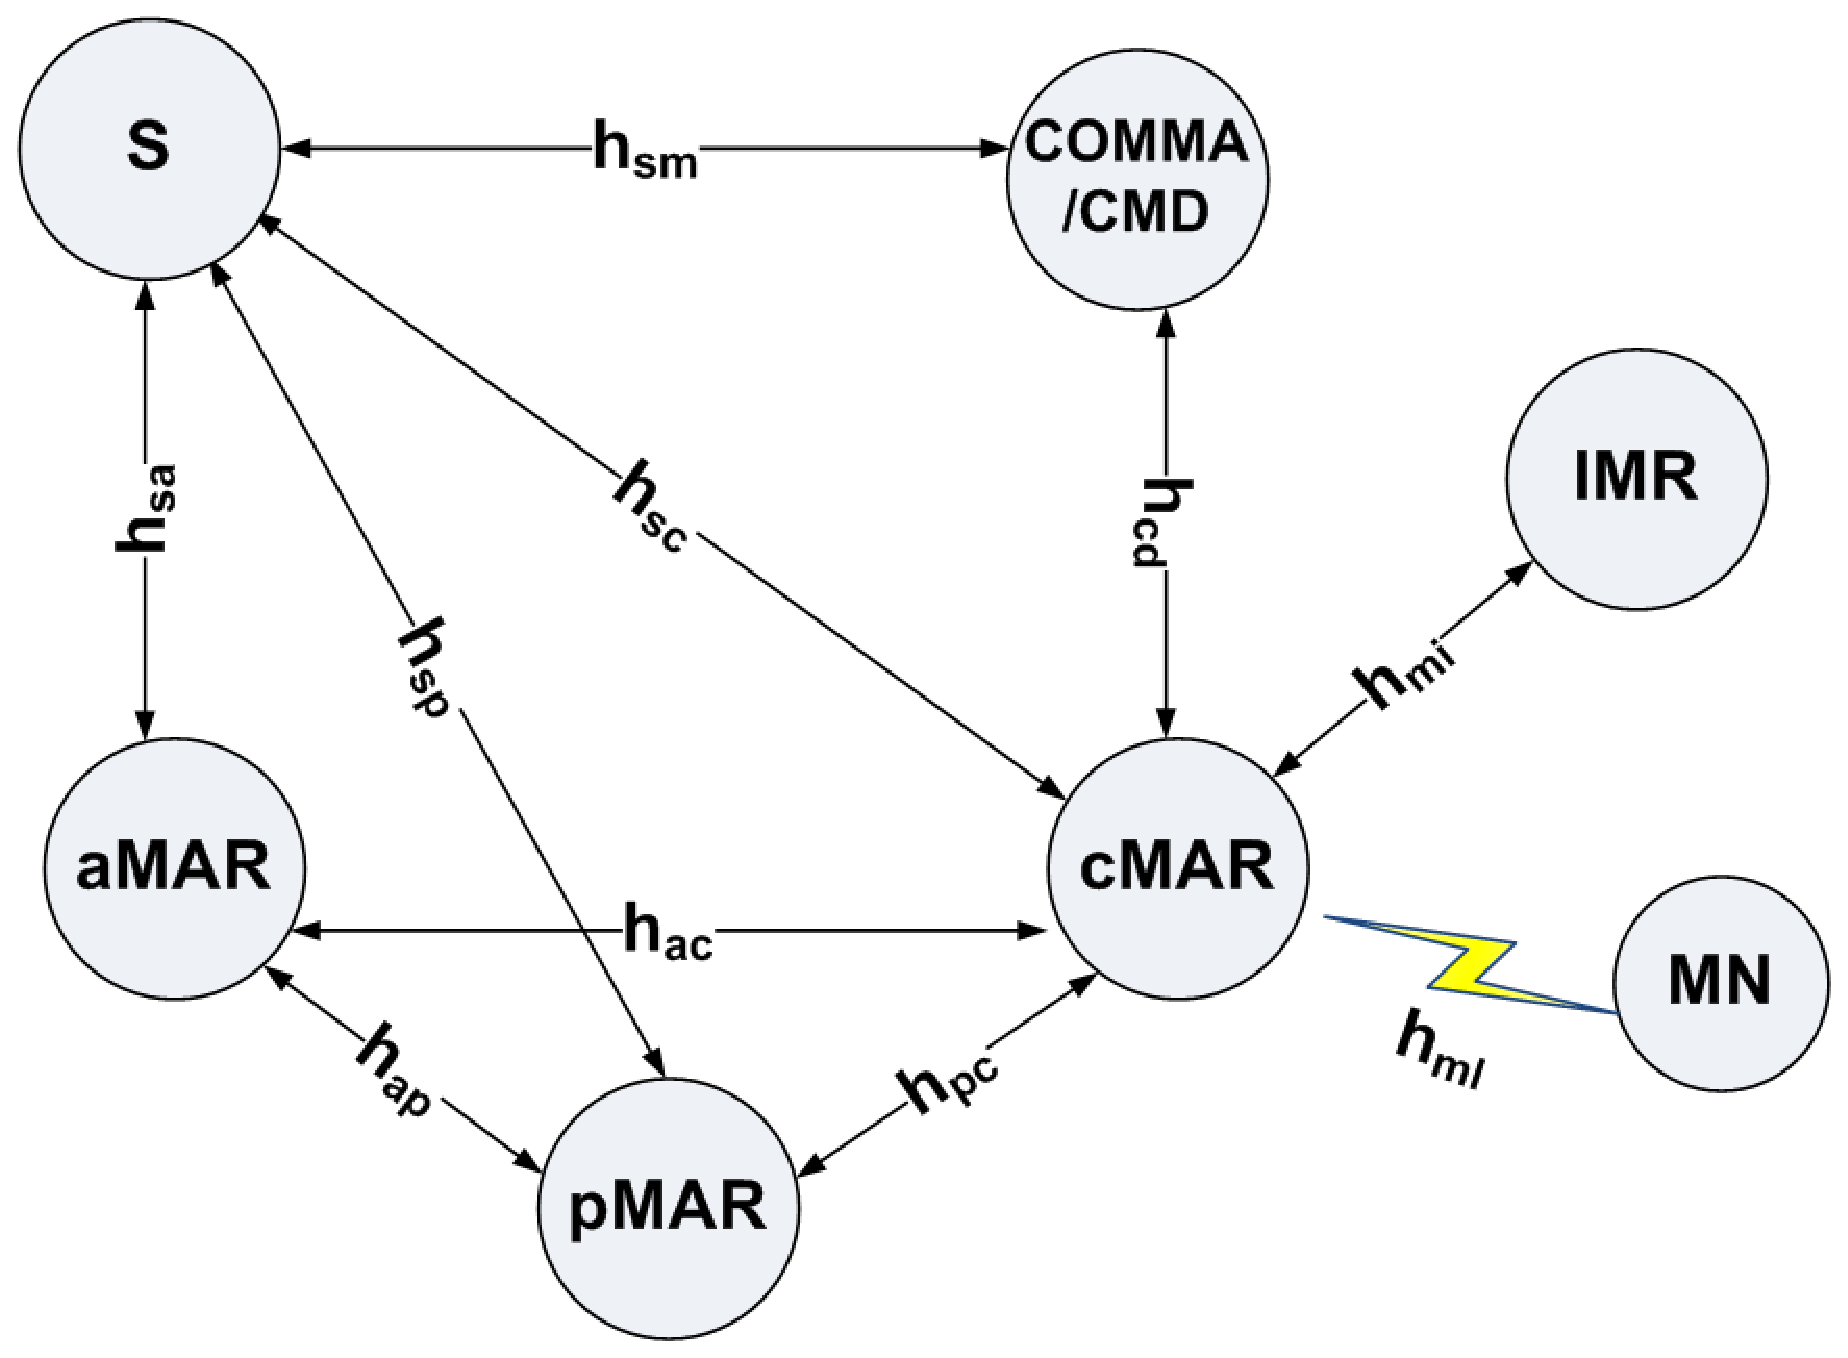
\includegraphics[width=0.55\textwidth]{./Part3/Chapter8/figures/c10_topology_analysis.eps} 
%    \caption{Une topologie de référence du réseau.}
%    \label{fig:c10_topology_analysis}
%  \end{center} 
%\end{figure}
%
%La figure~\ref{fig:c10_topology_analysis} présente une topologie de référence et les distances en saut entre les entités pour l'analyse de performance. A noter que l'intersection MR (IMR) est un router qui possède déjà un état ​​d'acheminement pour le groupe.
%On définit alors l'échelle du réseau $\psi$ qui est le ratio entre le nombre de sauts entre deux MAR adjacents ($h_{mm}$) et le nombre de sauts entre le MAR et le CMD ($h_{cd}$) . \\
%\begin{equation}
%\psi = \frac{h_{mm}}{h_{cd}}.
%\end{equation} 
%En règle générale, le nombre moyen de sauts entre deux MAR adjacents est inférieur à celui entre un MAR et une entité centralisée. Cela signifie que $ \psi \leq 1 $. Dans ce document, nous allons étudier l'impact de l'échelle du réseau sur les métriques de la performance en variant la valeur de $ \psi $ sur un intervalle [0,1].
%
%\paragraph{Les messages liés à l'analyse de performance}
%Dans notre analyse, différents messages sont utilisés. Pour un souci de simplicité, nous supposons qu'il existe un seul flux continu. $L_{RS}$, $L_{RA}$, $L_{PBU}$, $L_{PBA}$, $L_{ePBU}$, $L_{ePBA}$, $L_{M-Req}$, $L_{M-Res}$, $L_{C-Req}$, $L_{C-Res}$, $L_{MLD-R}$, $L_{Join}$, $L_{MP}$, $L_{T}$ est la taille du message Router Solicitation (RS), Router Advertisement (RA), PBU, PBA, PBU étendu, PBA étendu, request de transfert de contexte, réponse de transfert de contexte, demande de configuration de canal, réponse de configuration de canal,  Rapport MLD, PIM Rejoignez, paquet multicast, l'en-tête de tunnel; respectivement.
%
%\paragraph{Le modèle de délai}
%Dans cette thèse, on adopte le modèle de délai de transmission de paquets dans \cite{packet_transmission_delay} dans lequel la transmission de paquets se compose la durée de transmission et le temps de propagation. Ainsi, le délai de transmission d'une liaison filaire peut être calculé comme
%\begin{equation}
%d_{wd}(l,h) = h (\dfrac{l}{BW_{wd}} + D_{wd}),
%\end{equation}
%Où h est la distance en saut entre deux nœuds, l est la taille du paquet, $ BW_{wd} $ est la bande passante de liaison filaire et $ D_{wd} $ est la latence du liaison filaire.
%
%Contrairement à la transmission filaire qui peut être considéré comme fiable, la liaison sans fil n'est pas fiable. Le délai de transmission sans fil est donc calculé comme \cite{packet_transmission_delay} \\
%\begin{equation}
%d_{wl}(l) = \dfrac{1}{1-q} (\dfrac{l}{BW_{wl}} + D_{wl}),
%\end{equation} 
%où q est la probabilité d'échec de liaison sans fil, $ BW_{wl} $ est la bande passante et $ D_{wl} $ est la latence de liaison sans fil.
%
%\paragraph{Le modèle de mobilité}
%Dans ce document, nous considérons le cas où le MN se déplace toujours de MAR à MAR comme s'ils étaient déployés linéaire (l'utilisateur est en train de s'éloigner du premier MAR et jamais s'attache vers un MAR précédemment visité). Il représente le pire des cas. Ainsi, nous avons
%$h_{ac}$ = $h_{ap}$ + $h_{pc}$.
%
%Soit $ N_{mar} $ représente le nombre moyen de MARs impliqués dans le transfert du trafic de données vers / depuis un MN. Dans notre contexte, $ N_{mar} $ est également le nombre de handovers. On obtient donc 
%\begin{equation}
%h_{ac} = N_{mar} h_{mm},
%\end{equation} 
%\begin{equation}
%h_{pc} = h_{mm}.
%\end{equation}
%Dans notre analyse, la valeur basse de $ N_{mar} $ représente le nœud avec la faible mobilité ou le scénario dans lequel le flux est à court durée. La valeur plus élevée de $ N_{mar} $ correspond à la forte mobilité ou le scénario dans lequel le flux est à long terme.
%
%\subsubsection{La modélisation analytique}
%Ce paragraphe développe un modèle d'analyse en ce qui concerne différents paramètres de performance. Dans cette analyse, nous considérons le cas normal et le cas où le proxy MLD supportant la capacité de multiples d'interfaces en amont. Nous soulignons ensuite les impacts et les avantages de l'utilisation de plusieurs interfaces sur ​​ces métriques.
%
%\paragraph{Le temps d'interruption du service}
%Le temps d'interruption ($ SD(.)$) est définie comme une période où un auditeur est incapable de recevoir les paquets multicast. En supposant que le temps associé au traitement des messages dans les entités de réseau (par exemple, le temps de traitement de PBU et de mise à jour de cache dans MAR) est inclus dans la valeur totale de chaque variable. Ensuite, le temps d'interruption est (voir la figure~\ref{fig:c10_HO}). \\
%\small
%\begin{multline}
%SD(.) = T_{L2} + d_{wl}(L_{RS}) + d_{wd}(L_{ePBU},h_{cd}) + d_{wd}(L_{ePBA},h_{cd}) + max \{ d_{wd}(L_{PBA}, h_{ac}) \\+ d_{wd}(L_{PBU}, h_{ac}), d_{wd}(L_{M-Req},h_{pc}) +d_{wd}(L_{M-Res},h_{pc})\} \\ +max \{d_{wl}(L_{MP}), T_{M}{(.)} + d_{wl}(L_{MP})\},
%\label{eq:sd}
%\end{multline}
%\normalsize
%où $ T_{L2} $ est la durée de handover de la couche 2, $T_{M} (.)$ est le temps nécessaire pour le cMAR d'adhérer et obtenir le premier paquet après le handover.
%
%En cas MMA\_cMAR, le cMAR doit obtenir le trafic à partir de l'IMR qui a déjà un état ​​d'acheminement pour ce groupe. Ainsi \\
%\small
%\[ T_{M}(cMAR) = \left\{ 
% \begin{array}{l l}
%   \overline{w}_{mr} \quad \small \text{if } h_{mi} =0,  \\
%   (h_{mi} +1) \overline{w}_{mr}+d_{wd}(L_{MLD-R}) + d_{wd}(L_{MP}) +  d_{wd}(L_{Join},h_{mi}-1) \\+d_{wd}(L_{MP},h_{mi}-1)   \quad \small \text{if }h_{mi} \geq 1. 
% \end{array} \right.\] 
%\normalsize 
%où $ \overline{w}_{m} $ est le délai dans lequel un MR (et un proxy MLD) doit rejoindre un flux multicast à chaque routeur intermédiaire dans l'Internet \cite{MPDSR}.
%
%En cas MMA\_pMAR, le pMAR a eu l'état pour ce flux. Nous avons \\
%\begin{equation}
%T_{M}(pMAR) = 2\overline{w}_{mr} +d_{wd}(L_{MLD-R}+L_{T},h_{pc})+d_{wd}(L_{MP} +L_{T},h_{pc}).
%\end{equation}
%
%En cas MMA\_aMAR, il y a deux possibilités : le cas normal (cas 1, correspond au mode par défaut), et le cas où le proxy MLD supportant plusieurs interfaces « en amont » est déployé dans MARs. Dans ce dernier cas, dans le pire des cas, l'aMAR doit rejoindre le canal multicast, conduisant à un délai supplémentaire. Soit $ p_{a} $ représentent la probabilité que cette situation se produit. En conséquence, $ T_{M}(.) $ est calculé comme \\
%\begin{equation}
%T_{M}(aMAR) =(1-p_{a}) T_{M}(aMAR-c1)  +p_{a} T_{M}(aMAR-wc),
%\end{equation}
%où
%\begin{equation}
%T_{M}(aMAR-c1) =2\overline{w}_{mr} +d_{wd}(L_{MLD-R}+L_{T},h_{ac})+d_{wd}(L_{MP} +L_{T},h_{ac}),
%\end{equation}
%\small
%\[T_{M}(aMAR-wc)  = \left\{ 
% \begin{array}{l l}
%   T_{M}(aMAR-c1)  \quad \small \text{if } h_{mi} =0,  \\
%    T_{M}(aMAR-c1)+ d_{wd}(L_{MLD-R})+ d_{wd}(L_{MP})  + d_{wd}(L_{Join},h_{mi}-1) \\+ (h_{mi}+1)  \overline{w}_{mr} +d_{wd}(L_{MP},h_{mi}-1)  \quad \small \text{if }h_{mi} \geq 1. 
% \end{array} \right.\] 
%\normalsize 
%Il est à noter que $ T_{M} (aMAR-c1) $ représente le temps d'interruption dans le mode par défaut, quand $ T_{M}(aMAR) $ montre l'impact de l'utilisation de proxy avec plusieurs interfaces sur ​​le temps d'interruption. En conséquence, $ SD(aMAR) $ peut être considéré comme un compromis entre l'interruption de service et le problème de la convergence.
%
%Dans le cas MMA\_COMMA, nous avons\\
%\begin{equation}
%T_{M}(COMMA)= 2\overline{w}_{mr}+  d_{wd}(L_{MLD-R}+L_{T}, h_{cd}) + d_{wd}(L_{MP}+L_{T}, h_{cd}).
%\end{equation}
%
%\paragraph{Le délai de bout en bout}
%Le délai de bout en bout ($E2E(.) $) est le délai de transmission de paquets de la source à l'auditeur. Dans le MMA\_cMAR, le cMAR reçoit le trafic multicast directement à partir de l'infrastructure multicast. Par conséquent, le délai de bout-en-bout est donné par \\
%\begin{equation}
%E2E(cMAR) = d_{wd}(L_{MP},h_{sc}) + d_{wl}(L_{MP}).
%\end{equation}
%
%Dans le cas MMA\_aMAR, le paquet multicast est acheminé depuis la source vers le cMAR via l'aMAR, représentant le mode par défaut. Nous avons \\
%\begin{equation}
%E2E(aMAR) = d_{wd}(L_{MP},h_{sa}) + d_{wd}(L_{MP}+L_{T},h_{ac}) + d_{wl}(L_{MP}).
%\end{equation}
%
%En cas MMA\_pMAR, le MAR reçoit toujours le trafic de son pMAR dans le cas normal. Par conséquent, le délai de bout-en-bout est donné comme suit \\
%\begin{equation}
%E2E(pMAR-c1)= d_{wd}(L_{MP},h_{sa}) + d_{wd}(L_{MP} +L_{T},h_{ap}) + d_{wd}(L_{MP} + L_{T},h_{pc})  + d_{wl}(L_{MP}).
%\end{equation}
%
%En cas d'utilisation de proxy avec plusieurs interfaces, nous supposons que $ p_{p} $ est la probabilité que le MAR obtient le trafic multicast d'une interface « en amont ». Ainsi, $ 1-p_{p} $ est la probabilité que le MAR obtient le trafic multicast de son pMAR. Le délai dans le cas MMA\_pMAR est donc donné par
%\begin{multline}
%E2E(pMAR)=   d_{wl}(L_{MP}) + [d_{wd}(L_{MP},h_{sa})+ N_{mar} d_{wd}(L_{MP} +L_{T},h_{mm})] p_{p}^{N_{mar}-1} \\+ \sum_{i=1}^{N_{mar}-1} [d_{wd}(L_{MP},h_{i})+ (N_{mar}-i) d_{wd}(L_{MP} +L_{T},h_{mm})] p_{p}^{N_{mar}-i-1} (1-p_{p}),
%\end{multline}
%où $ h_{i} $ est la distance en saut de la source vers le i$^{ième} $ MAR dans le chemin de déplacement du MN (de l'aMAR au cMAR), par exemple, $ h_{N_{mar}-1} = h_{sp}$.  
%
%Considérant le MMA\_COMMA, le délai de bout en bout est exprimé sous la forme \\
%\begin{equation}
%E2E(COMMA) = d_{wd}(L_{MP},h_{sm})  + d_{wd}(L_{MP}+L_{T},h_{cd}) + d_{wl}(L_{MP}).
%\end{equation}
%
%\paragraph{L'analyse du coût}
%Dans ce paragraphe, le coût de signalisation ($ SC (.) $), le coût de livraison de paquets ($ PC (.) $) et le coût de tunnelisation ($ TC (.) $) sont étudiés. Le coût de signalisation (per handover) est le frais général de signalisation pour soutenir le handover y compris les procédures relatives au multicast. Il peut être calculé comme \\
%\begin{equation}
%SC(.) =SC_{LU} + SC_{M}(.),
%\end{equation}
%où $ SC_{LU}$, $ SC_{M} (.) $ est le coût pour la mise à jour de l'emplacement et les procédures relatives au multicast, respectivement. Le coût de signalisation est calculé comme le produit de la taille du message, la distance et le coût de transmission d'une unité dans une liaison filaire/sans fil ($ \alpha $ pour le liaison filaire et $\beta $ pour la liaison sans fil). $ SC_{LU} $ est donc donné par \ \
%\begin{equation}
%SC_{LU} = \beta (L_{RS} + L_{RA}) + \alpha (L_{ePBU}  h_{cd} + L_{ePBA} h_{cd})  + \alpha (L_{PBU}  h_{ac} + L_{PBA} h_{ac}).
%\end{equation}
%$SC_{M}(.)$ est calculé par\\
%\begin{equation}
%SC_{M}(cMAR) = \alpha  (L_{M-Req}  h_{pc} + L_{M-Res} h_{pc} + L_{MLD-R} + L_{Join} h_{mi}).
%\end{equation}
%\begin{equation}
%SC_{M}(pMAR) = \alpha (L_{M-Req}  h_{pc} + L_{M-Res} h_{pc} + L_{MLD-R} h_{pc}).
%\end{equation}
%\begin{equation}
%SC_{M}(aMAR) =(1-p_{a}) SC_{M}(aMAR-c1)  + p_{a} SC_{M}(aMAR-wc),
%\end{equation}
%où 
%\begin{equation}
%SC_{M}(aMAR-c1) = \alpha (L_{M-Req}  h_{pc} + L_{M-Res} h_{pc} +L_{MLD-R} h_{ac}),
%\end{equation}
%\begin{equation}
%SC_{M}(aMAR-wc) = \alpha (L_{M-Req}  h_{pc} + L_{M-Res} h_{pc}  + L_{MLD-R} h_{ac}+L_{MRD-R} +L_{Join} h_{mi}).
%\end{equation}
%
%\begin{equation}
%SC_{M}(COMMA) = \alpha (L_{M-Req}  h_{pc} + L_{M-Res} h_{pc}  + L_{MLD-R} h_{cd}).
%\end{equation}
%
%Le coût de livraison représente le coût de livraison des paquets multicast pour le MN par unité de temps. Soit $ S_{c} $, $\lambda_{p} $ représentent la durée moyenne des séances au cMAR et le taux d'arrivée des paquets, respectivement. Encore, le coût dans le MMA\_aMAR correspond au mode par défaut. Le coût est exprimé sous la forme \\
%\begin{equation}
%PC(cMAR) = S_{c} \lambda_{p} (\alpha L_{MP} h_{sc}  + \beta L_{MP}).
%\end{equation}
%\begin{equation}
%PC(aMAR) = S_{c} \lambda_{p} [\alpha L_{MP} h_{sa} + \alpha (L_{MP} + L_{T}) h_{ac}  + \beta L_{MP}].
%\end{equation}
%
%En cas MMA\_pMAR, dans le cas normal, le MAR reçoit toujours le trafic multicast de son pMAR. Ainsi, le coût de livraison de paquets est donné comme suit \\
%\begin{equation}
%PC(pMAR-c1)=  S_{c} \lambda_{p} [\alpha  L_{MP} h_{sa} +  \alpha  (L_{MP} + L_{T}) ( h_{ap} + h_{pc}) + \beta L_{MP}].
%\end{equation}
%En utilisant le proxy avec multiples interfaces, le coût de livraison est calculé comme étant
%\begin{multline}
%PC(pMAR)= S_{c} \lambda_{p}  \beta L_{MP} +  S_{c} \lambda_{p} [\alpha L_{MP} h_{sa}+ \alpha N_{mar}  (L_{MP} +L_{T}) h_{mm}] p_{p}^{N_{mar}-1} \\+ S_{c} \lambda_{p} \sum_{i=1}^{N_{mar}-1} [\alpha L_{MP} h_{i}+ \alpha  (N_{mar}-i) (L_{MP} +L_{T}) h_{mm}] p_{p}^{N_{mar}-i-1} (1-p_{p}).
%\end{multline}
%
%En cas MMA\_COMMA, le coût de livraison de paquets est \\
%\begin{equation}
%PC(COMMA) = S_{c} \lambda_{p} [\alpha L_{MP} h_{sm} + \alpha (L_{MP} + L_{T}) h_{cd}  + \beta L_{MP}].
%\end{equation}
%
%En ce qui concerne le coût de tunnelisation, il est défini comme le coût supplémentaire de la tête de tunnel. En MMA\_cMAR, le trafic multicast est reçu directement à partir de l'infrastructure multicast, il n'y a donc pas de coût de tunnelisation. Au contraire, dans les cas MMA\_aMAR, MMA\_pMAR et MMA\_COMMA le trafic est routé via le tunnel aMAR-cMAR, pMAR-cMAR, et cMAR-COMMA, respectivement. A noter que le coût de tunnelisation dans le cas MMA\_aMAR correspond au mode multicast par défaut. Le coût de tunnelisation est donc calculé comme \\
%\begin{equation}
%TC(cMAR) = 0. 
%\end{equation}
%\begin{equation}
%TC(aMAR) = \alpha  S_{c} \lambda_{p} (L_{MP} + L_{T}) h_{ac}. 
%\end{equation}
%\begin{equation}
%TC(pMAR)=  \alpha  S_{c} \lambda_{p} (L_{MP} + L_{T}) h_{mm}  \sum_{i=0}^{N_{mar-1}} (N_{mar}-i)p_{p}^{N_{mar}-i-1} (1-\theta p_{p}).
%\end{equation}
%où  
%\[\theta  = \left\{ 
% \begin{array}{l l}
%   0 \quad \small \text{if } i =0,  \\
%    1  \quad \small \text{if } i \geq 1. 
% \end{array} \right.\] 
%
%\begin{equation}
%TC(COMMA) = \alpha  S_{c} \lambda_{p} (L_{MP} + L_{T}) h_{cd}. 
%\end{equation}
%
%Le coût de signalisation en général, est un facteur important qui influence l'évolutivité du réseau. Cependant, en tant que le plan de données et le plan de contrôle ne sont plus couplés, dans le cas où une grande quantité de trafic est générée dans le réseau, le coût de livraison de paquets et le coût de tunnelisation jouent le rôle plus important.
% 
%\paragraph{La perte de paquets}
%Pendant le handover, les paquets peuvent être perdus. Le nombre de paquets perdus est proportionnel à la durée de l'interruption du service, et le taux d'arrivée des paquets. En conséquence, le nombre de paquets perdus est donné par \\
%\begin{equation}
%\varphi_{p}(.)= \lambda_{p} SD(.).
%\end{equation}
%
%\normalsize
%\subsubsection{Les résultats numériques}
%Ce paragraphe présente les résultats numériques basés sur l'analyse donnée dans le paragraphe précédent. Les valeurs des paramètres par défaut sont présentées dans le tableau \ref{tap:c10_parameters}, dans lequel $L_{PBU}$,  $L_{PBA}$, $L_{ePBU}$, $L_{ePBA}$, $L_{M-Req}$, $L_{M-Res}$, $L_{C-Req}$ et $L_{C-Res}$ sont extraites de l'implémentation réelle de PMIPv6 \cite{oai_pmip} et de fonction de transfert de contexte \cite{d4.4}, tandis que les autres sont de \cite{HO_comparison_Lee, DMM_analysis_Hassan, dsrm, d4.4}. Il est à noter que le $ SD (aMAR-c1) $, $ E2E (aMAR) $, $ SC (aMAR-c1) $, $ PC (aMAR) $ et $ TC (aMAR) $ correspondent au mode par défaut dans notre analyse. \\
%\begin{table}[ht]
%\small
%\caption{Paramètres pour l'analyse de la performance.}
%\label{tap:c10_parameters}
%\centering
%\begin{tabular}{|c |c |c |c |c |c |}%{|l|l|l|l|l|l|}%
%\hline
%\textbf{Paramètre} & \textbf{Valeur} & \textbf{Paramètre} & \textbf{Valeur} & \textbf{Paramètre} & \textbf{Valeur}  \\
%\hline
%$T_{L2}$ & 50ms & $BW_{wd}$  &  100Mbps & $BW_{wl}$  & 11 Mbps\\
%\hline
%  $D_{wd}$& 2ms  & $D_{wl}$ & 10ms & $q$& 0.35  \\
%\hline
%$\overline{w}_{mr}$&  10 ms  & $h_{mm}$ & 3 sauts & $h_{cd}$&  12 sauts  \\
%\hline
%$h_{mi}$& 2 sauts  & $h_{sa}$& 16 sauts  & $h_{sp}$&  16 sauts   \\
%\hline
% $h_{sc}$  & 16 sauts   & $h_{sm}$&  16 sauts &$S_{c} $&  60 s  \\
%%\hline
%%$h_{cm}$& 12 hops  & $R$& 500m  & 1/$\mu_{s}$&  600s  \\
%\hline
%$\lambda_{p}$& 10 paquets/s  & $\alpha$&  1 & $\beta $&  5  \\
%\hline
%$p_{p}$& 0.9  & $p_{a}$&  0.5 & $L_{RS}$ & 52 octets \\
%\hline
% $L_{RA}$& 80  & $L_{PBU}$& 84 & $L_{PBA}$ & 92 octets \\
%\hline
% $L_{ePBU}$&  84 octets  & $L_{ePBA}$, & 128 octets & $L_{M-Req}$ & 86 octets \\
%\hline 
%$L_{M-Res}$ & 104 octets  & $L_{C-Req}$ & 92 octets & $L_{C-Res}$ & 112 octets \\
%\hline
%$L_{MLD-R}$ & 96 octets  &$L_{Join}$ & 110 octets & $L_{MP}$ &  200 octets \\ 
%\hline
% $L_{T}$ & 40 octets  & &  & &   \\ 
%\hline
%\end{tabular}
%\end{table}
%\normalsize
%\paragraph{Le temps d'interruption de service multicast}
%\begin{figure}[!h]
%\centering
%\subfloat[]{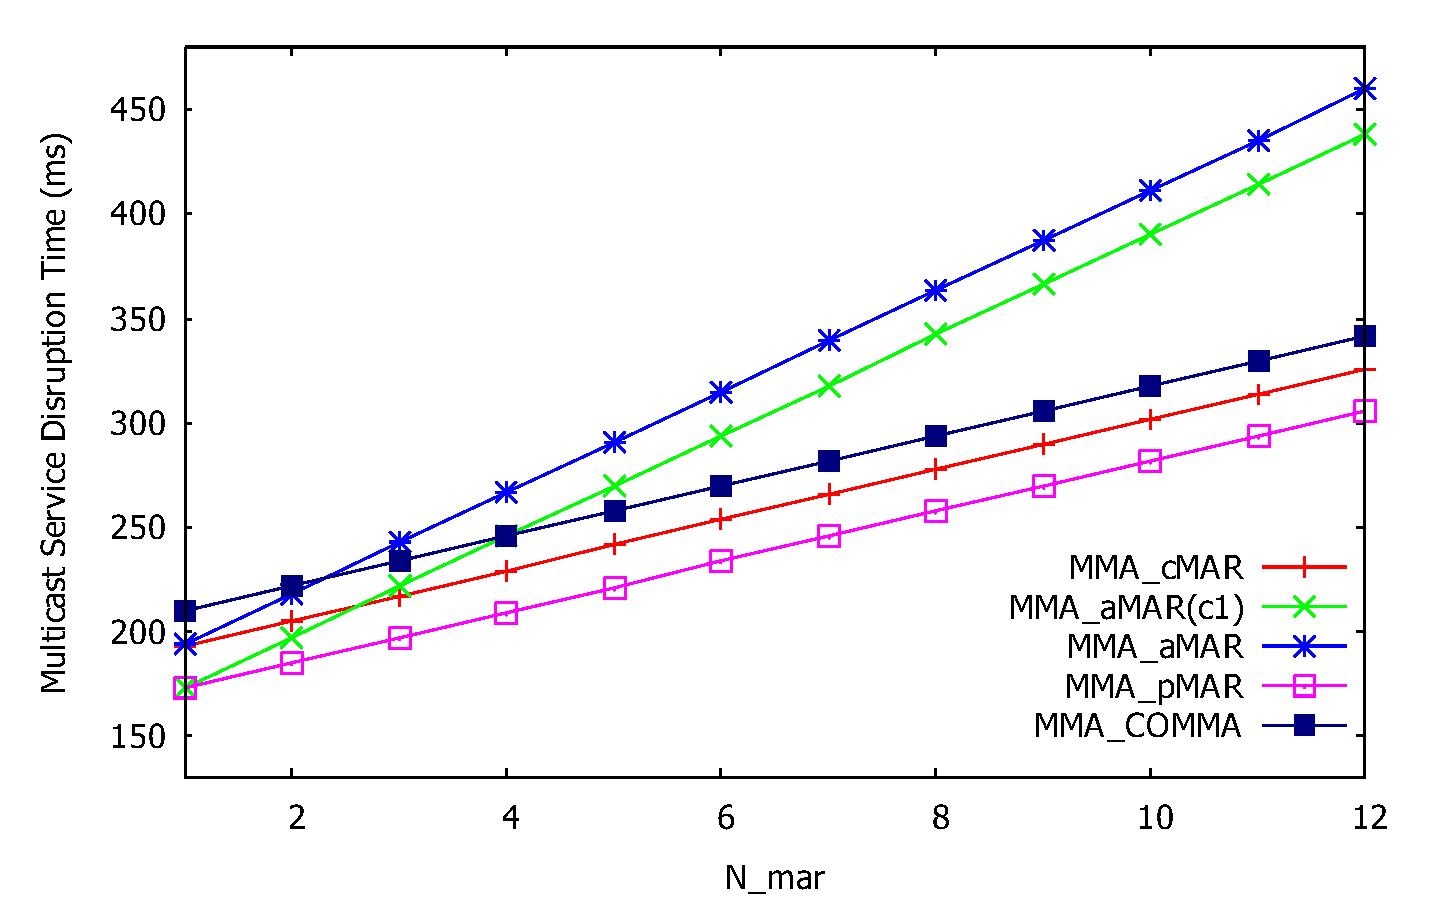
\includegraphics[scale=0.28]{./Part3/Chapter8/figures/c10_sd_n_mar.eps} \label{fig:c10_sd_n_mar}}
%\subfloat[]{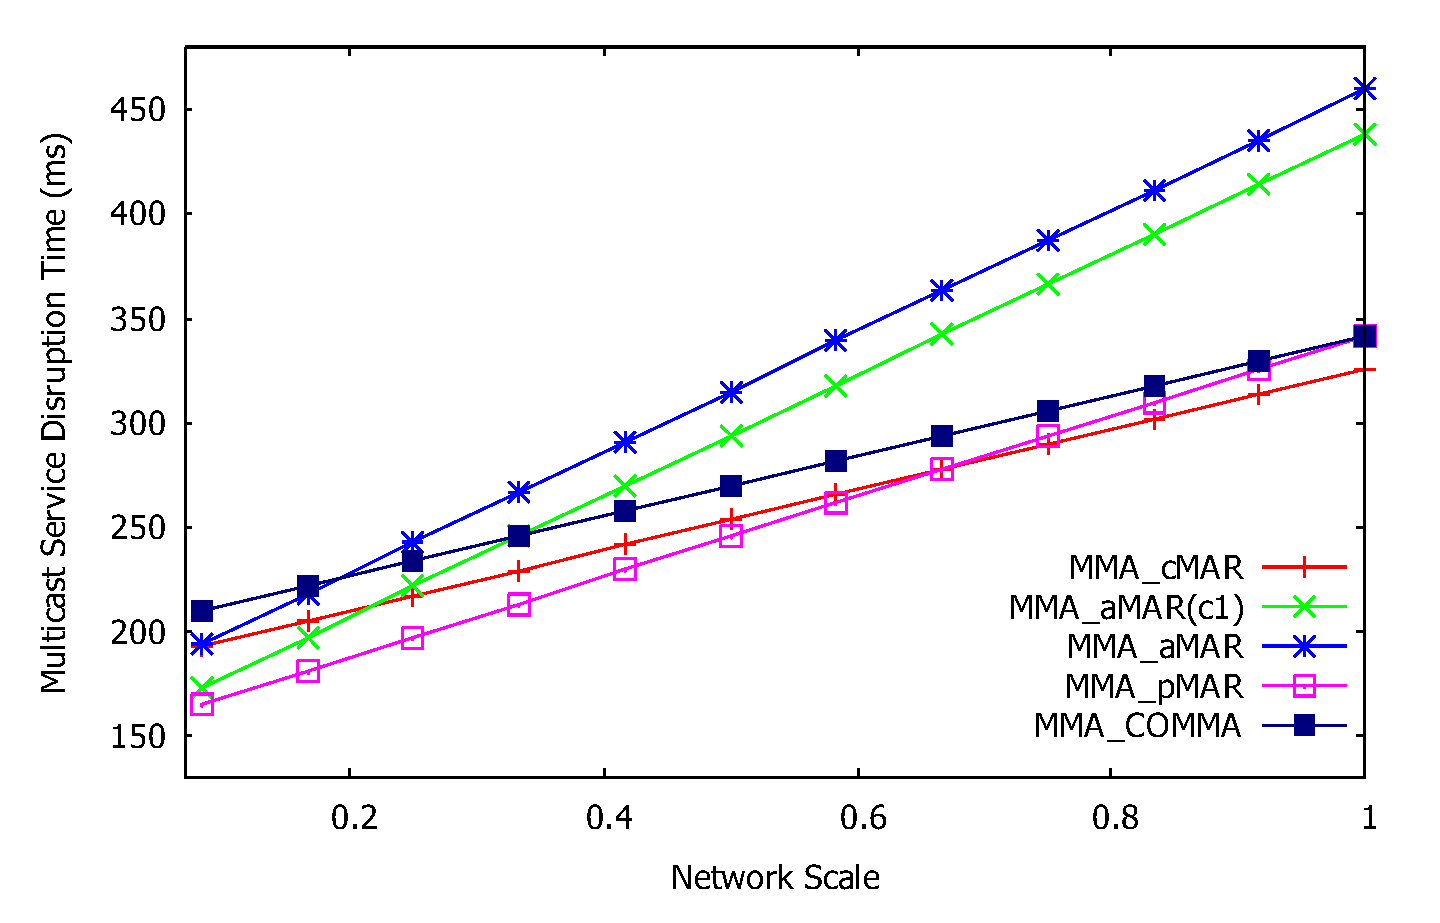
\includegraphics[scale=0.28]{./Part3/Chapter8/figures/c10_scale.eps}\label{fig:c10_scale}}\,
%\subfloat[]{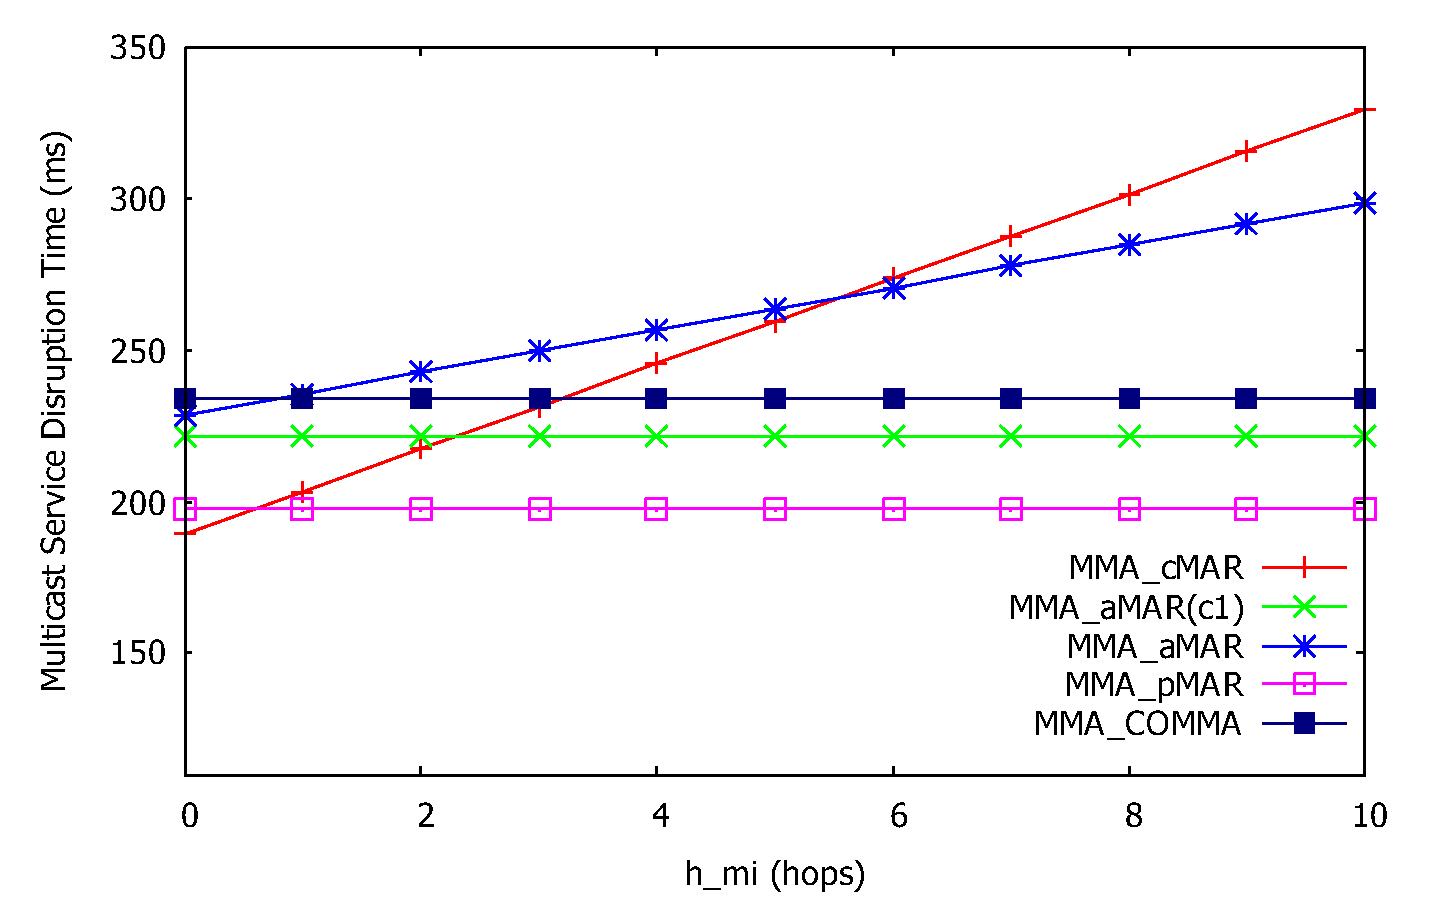
\includegraphics[scale=0.28]{./Part3/Chapter8/figures/c10_h_mi.eps}\label{fig:c10_h_mi}}
%\caption[Le temps d'interruption de service multicast.]{Le temps d'interruption comme une fonction de : (a) $N_{mar}$, (b) $\psi$, (c) $h_{mi}$.} 
%\label{fig:c10_sd}
%\end{figure}
%La figure ~\ref{fig:c10_sd_n_mar} montre le temps d'interruption de service quand $ N_{mar} $ est variée sur une intervalle de 1 à 12. Il apparaît clairement que l'approche MMA\_pMAR donne une meilleure performance que les autres. Lorsque $ N_{mar} $ est faible (moins de 5), toutes les approches satisfont à l'exigence en termes d'interruption pour les services en temps réel (inférieur à 300 ms). Lorsque $ N_{mar} $ est relativement grande, l'interruption de service en cas MMA\_aMAR est significativement augmentée. Nous étudions aussi l'impact de l'échelle du réseau ($\psi $) sur le temps d'interruption. Dans ce cas, $ N_{mar} $ est réglée à une valeur de 3. D'une manière générale, l'impact de $\psi $ est similaire à celui de $ N_{mar} $. Surtout, Fig.~\ref{fig:c10_scale} montre qu'il existe une zone où le MMA\_cMAR surpasse le MMA\_pMAR (lorsque $\psi  \geq 0.62$).\\
%La figure~\ref{fig:c10_h_mi} indique le temps d'interruption lorsque $ h_{mi} $ est variée sur une intervalle de 0 à 10 sauts. Une petite valeur de $ h_{mi} $ indique un scénario de forte densité d'auditeur et une valeur élevée de $ h_{mi} $ représente un scénario de faible densité d'auditeur. Le temps d'interruption dans le MMA\_pMAR est plus faible que dans les autres (sauf si $ h_{mi} = 0 $ indiquant le cas où le trafic multicast est déjà disponible au MR « en amont » du cMAR). Comme la valeur de $ h_ {mi} $ augmente, le temps d'interruption dans le MMA\_pMAR, MMA\_aMAR (c1) et MMA\_COMMA est maintenu constant alors que celui dans les autres cas est considérablement augmenté. Par conséquent, la différence entre les approches est augmentée. En outre, le temps d'interruption dans MMA\_cMAR dépend fortement de la valeur de $ h_{mi} $. En d'autres termes, il ne peut pas être garantie à l'approche MMA\_cMAR. En outre, dans MMA\_aMAR, il augmente de manière significative comparé à celui dans le cas MMA\_aMAR (c1) à la suite de l'utilisation du proxy avec plusieurs interfaces.\\
%\begin{figure}[h!]
%\centering
%\subfloat[]{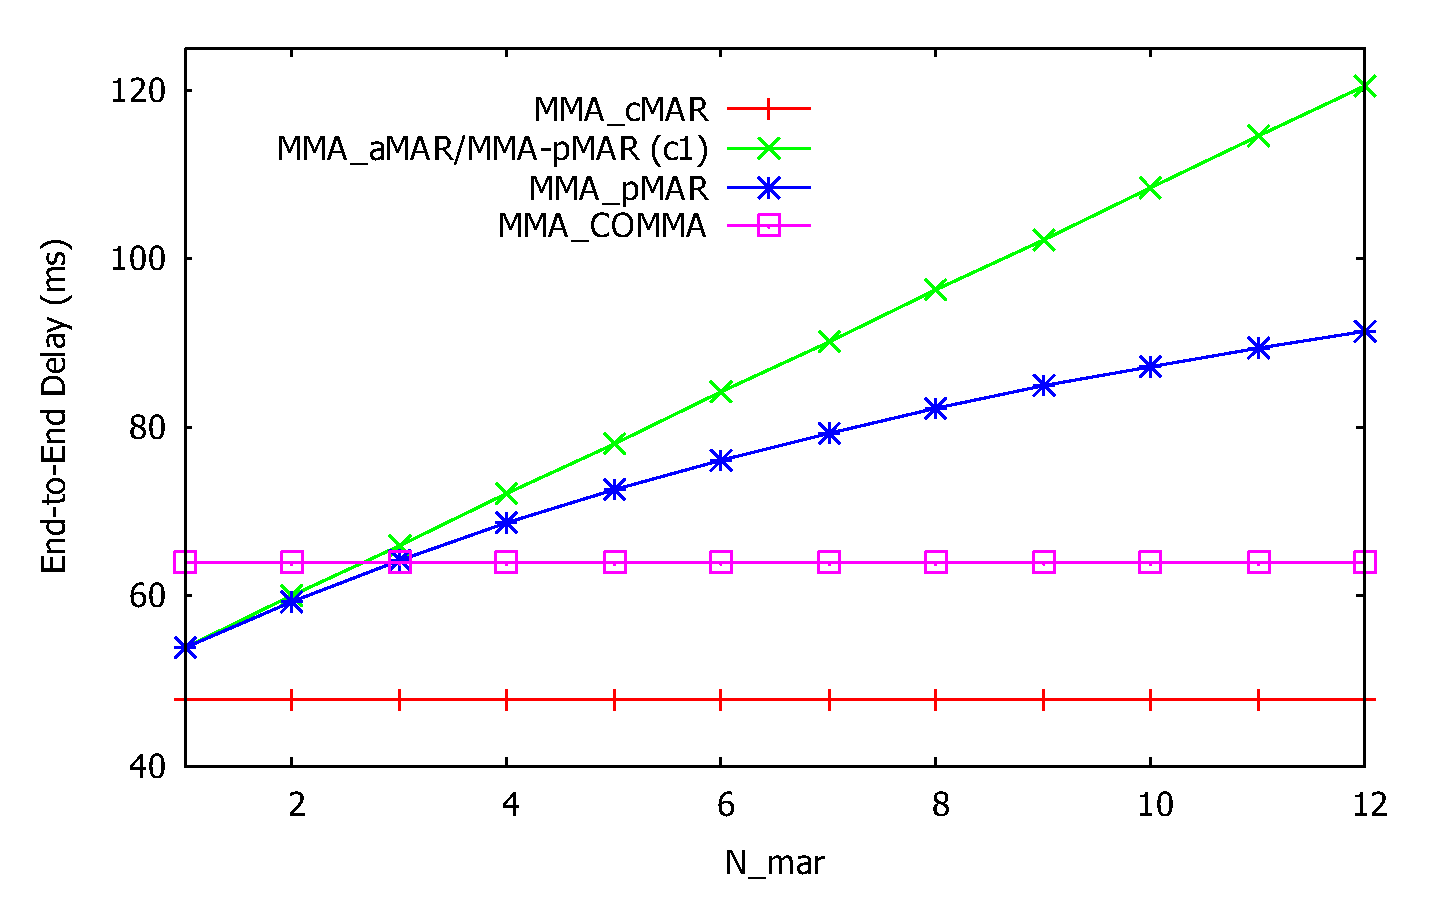
\includegraphics[width=0.50\textwidth]{./Part3/Chapter8/figures/c10_e2e_n_mar.eps} \label{fig:c10_e2e_n_mar}}
%\subfloat[]{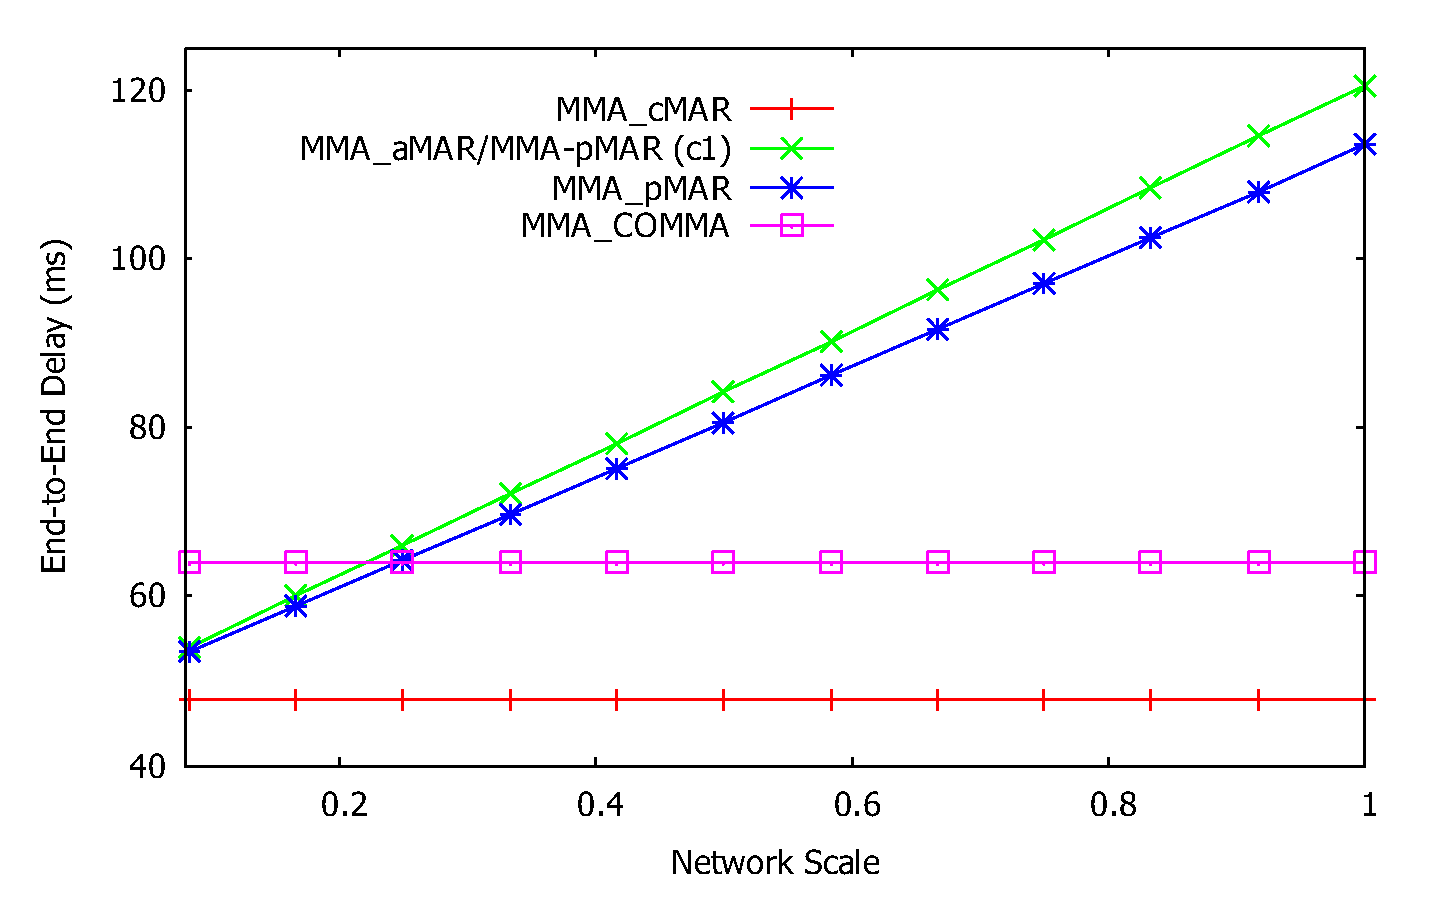
\includegraphics[width=0.50\textwidth]{./Part3/Chapter8/figures/c10_e2e_scale.eps}\label{fig:c10_e2e_scale}}\,
%\subfloat[]{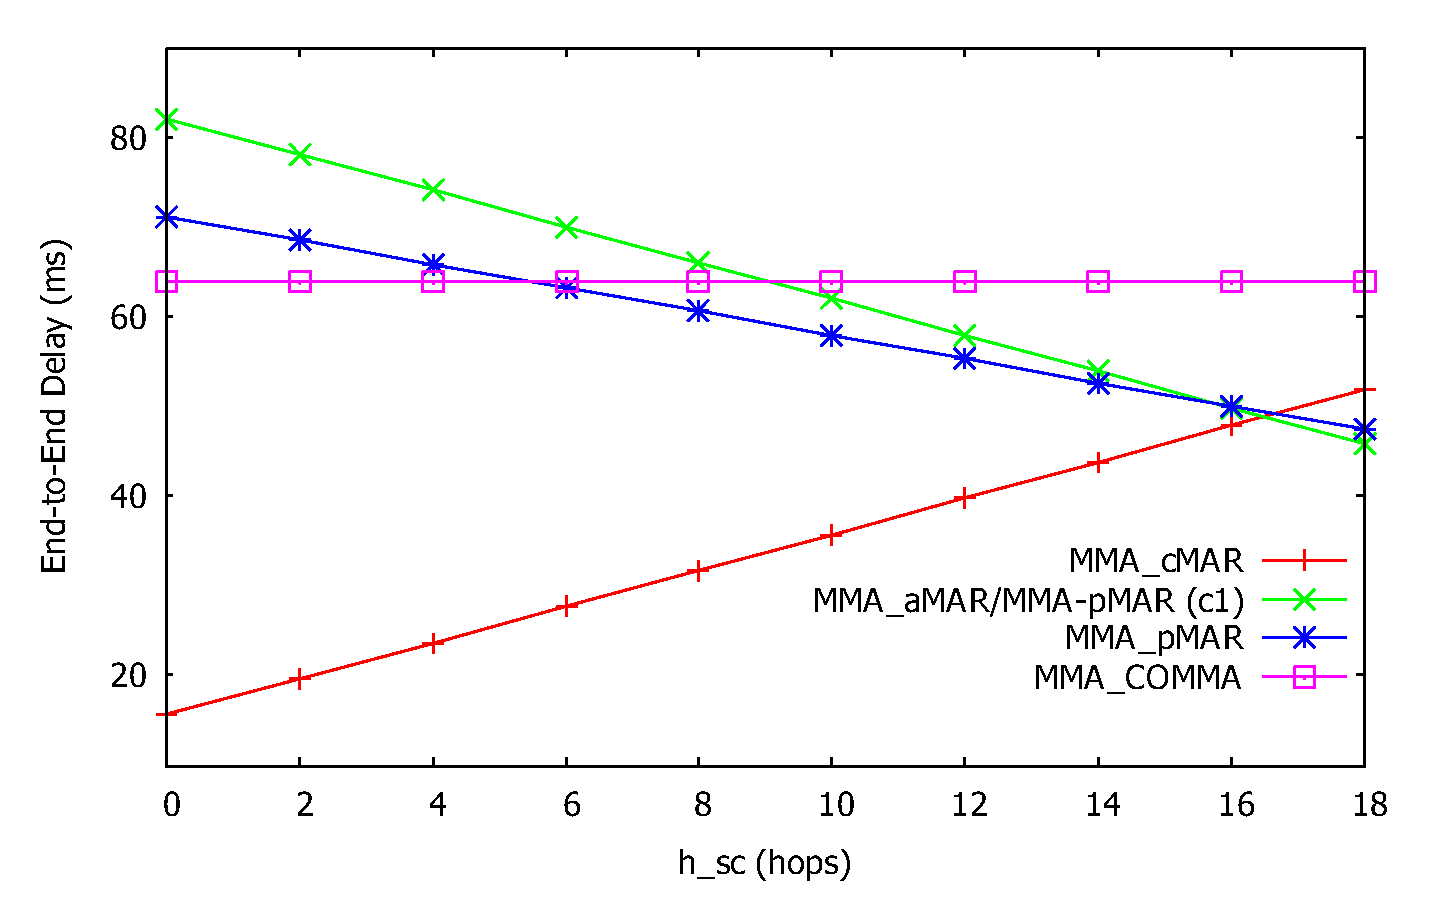
\includegraphics[width=0.50\textwidth]{./Part3/Chapter8/figures/c10_e2e_h_sc.eps}\label{fig:c10_e2e_h_sc}}
%\caption[Le délai de bout en bout.]{Le délai de bout en bout en fonction de : (a) $N_{mar}$, (b) $\psi$, (c) $h_{sc}$.}
%\label{fig:c10_e2e}
%\end{figure}
%En conclusion, l'approche MMA\_pMAR est généralement bien adaptée pour les services sensibles à l'interruption. Ainsi, l'augmentation du temps d'interruption, qui est causée par les multiples interfaces, peut être considérée comme un compromis entre le temps d'interruption et le problème de la convergence.
%\paragraph{Le délai de bout en bout}
%Maintenant, nous étudions l'impact de $ N_{mar} $ sur le délai de bout-en-bout. La figure ~\ref {fig:c10_e2e_n_mar} montre le délai par rapport au nombre de handovers $ N_{mar} $. Comme $ N_{mar} $ augmente ($h_ {ca} $ augmente) le délai en cas MMA\_aMAR et MMA\_pMAR augmente rapidement, tandis que celui dans MMA\_cMAR et MMA\_COMMA est maintenu constant. A noter que le délai dans MMA\_cMAR est maintenu en dessous de la valeur de 50 ms. Cela signifie que MMA\_cMAR satisfait à la exigence stricte en termes de délai de bout-en-bout. Le délai dans MMA\_pMAR (c1) est supérieur à celui dans le MMA\_pMAR à la suite de l'utilisation de multiples interfaces « en amont ». Comme on peut le voir sur la figure~\ref{fig:c10_e2e_scale}. En général, l'échelle du réseau a un impact similaire sur le délai de bout en bout que $ N_{mar} $. La différence majeure est que l'augmentation de la ligne MMA\_pMAR dans la figure~\ref{fig:c10_e2e_scale} est plus rapide que celle dans la figure~\ref{fig:c10_e2e_n_mar}.\\
%Ensuite, $ N_{mar} $ est réglé à une valeur de 6 (correspondant aux flux à moyen / long terme et aux nœuds à moyen / haute mobilité), tandis que la valeur de $ h_ {sc} $ est variée. A ce stade, nous supposons que $h_{sa}$ + $h_{sc} $ est une valeur fixe, par exemple, 18 sauts et $ h_{sp} $ = $ h_{sc} $. Ce scénario est utilisé pour illustrer le cas où la source est très proche de l'aMAR (côté droit de la figure~\ref {fig:c10_e2e_h_sc}) ou  très proche du cMAR (côté gauche de la figure~\ref {fig:c10_e2e_h_sc}). Comme on peut le voir sur la figure~\ref {fig:c10_e2e_h_sc}, même lorsque la source est très proche de l'aMAR, l'approche MMA\_cMAR donne une meilleure performance en termes de délai de bout en bout que les autres. Ainsi, l'impact du tunnel de la mobilité sur le délai est évident. En conclusion, le cMAR est généralement bien adapté pour les flux sensibles aux délais.
%\begin{figure}[h!]
%\centering
%\subfloat[]{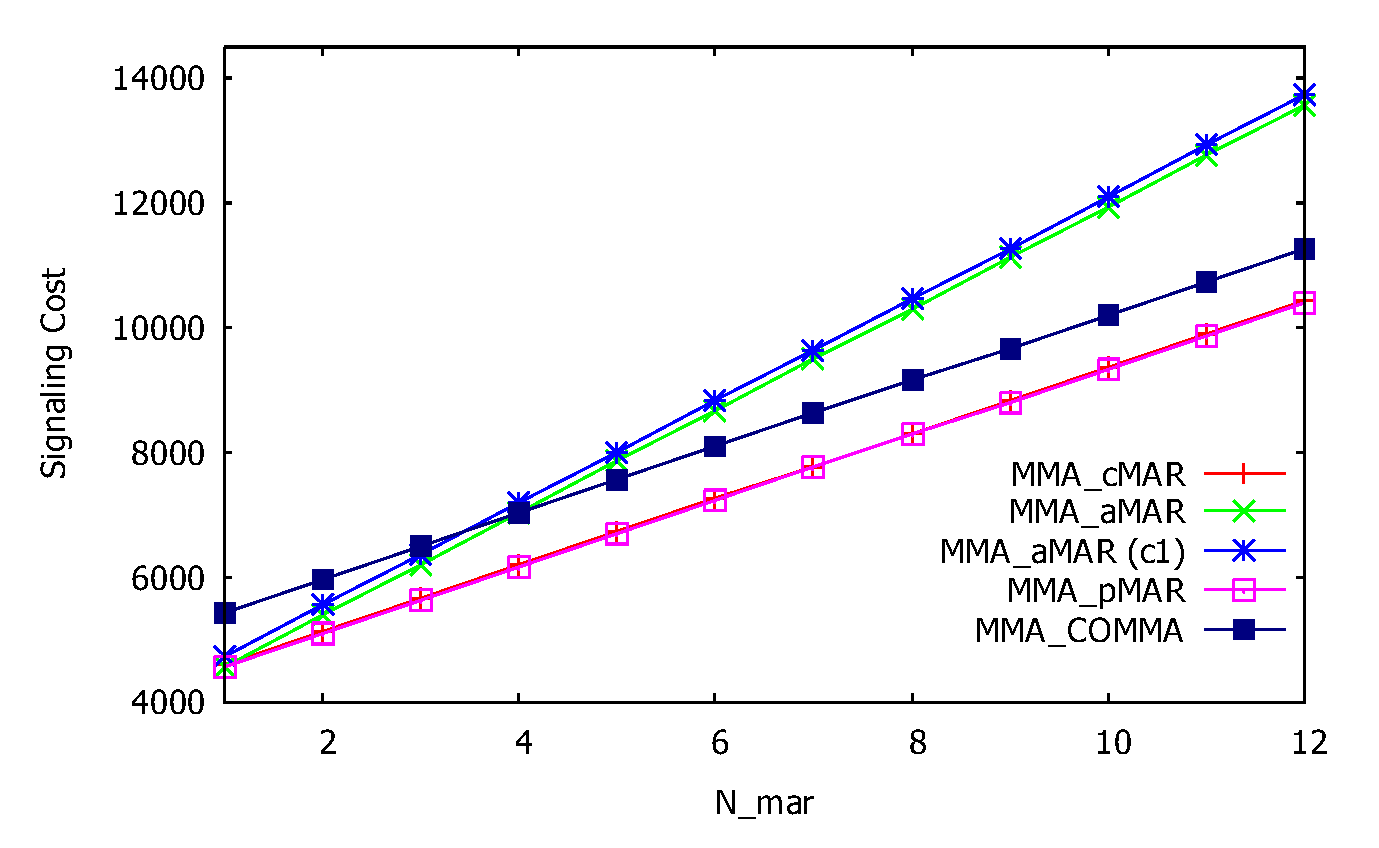
\includegraphics[width=0.50\textwidth]{./Part3/Chapter8/figures/c10_sc_n_mar.eps} \label{fig:c10_sc_n_mar}}
%\subfloat[]{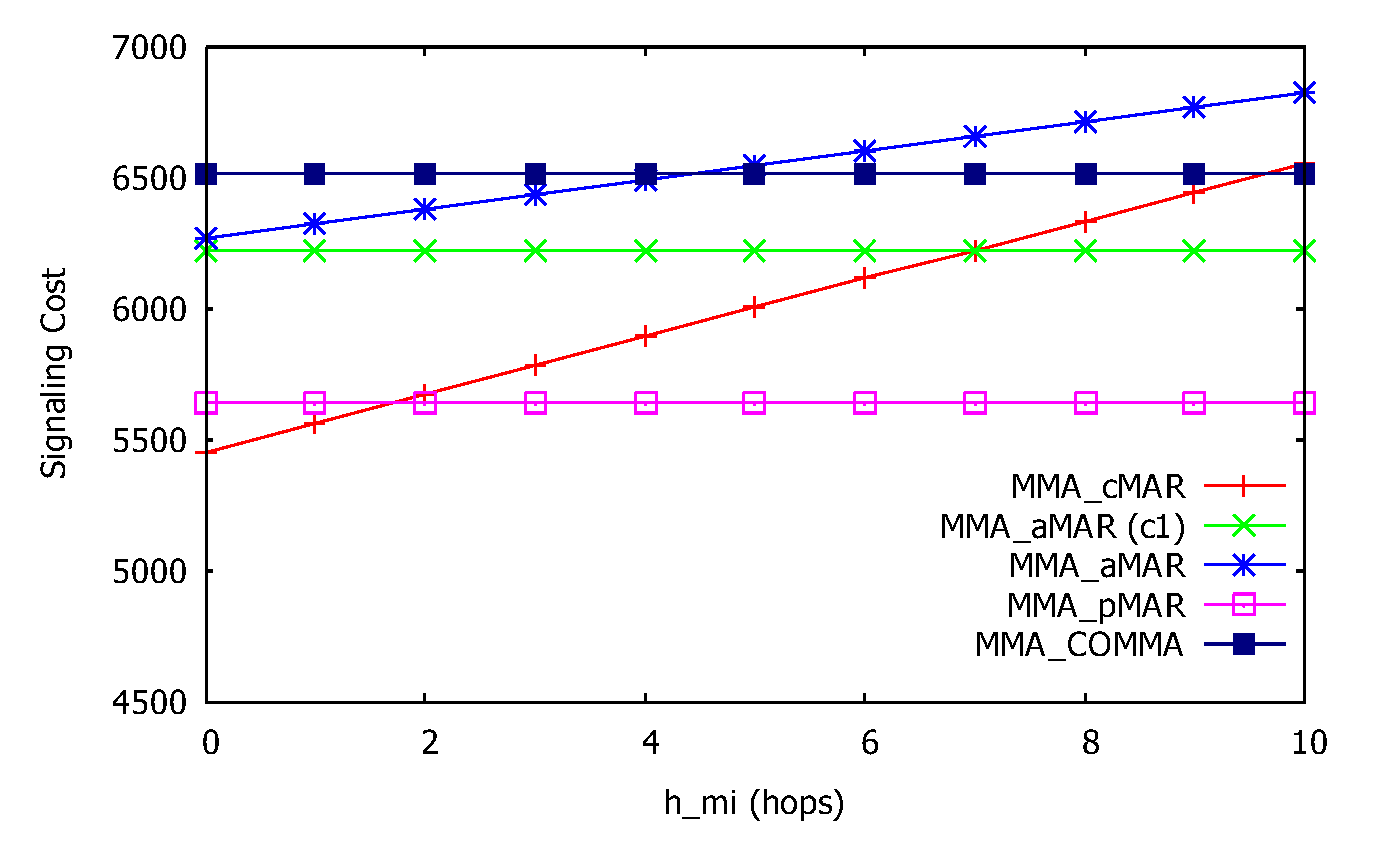
\includegraphics[width=0.50\textwidth]{./Part3/Chapter8/figures/c10_sc_h_mi.eps}\label{fig:c10_sc_h_mi}}
%\caption[Le coût de signalisation.]{Le coût de signalisation comme une fonction de: (a) $N_{mar}$, (b) $h_{mi}$.}
%\label{fig:c10_sc}
%\end{figure}
%\paragraph{Le coût de signalisation}
%La figure~\ref{fig:c10_sc} montre le coût de signalisation en fonction de $ N_{mar} $ et $ h_ {mi} $. En général, le coût de signalisation augmente lorsque $ N_{mar} $ augmente. Sur la figure~\ref{fig:c10_sc_n_mar}, le coût de signalisation dans le cas MMA\_cMAR et MMA\_pMAR est inférieur à celui dans les autres cas. Quand $ N_{mar} $ est assez petite, le coût de signalisation en cas MMA\_COMMA devient plus élevé. Dans le cas contraire, le coût en cas MMA\_aMAR devient plus élevé. Comme on peut le voir sur la figure~\ref{fig:c10_sc_h_mi} (quand $ h_ {mi} $ est variée), le MMA\_pMAR surpasse les autres quand $ h_{mi} $ est supérieur à 2.
%\paragraph{Le coût de livraison de paquets}
%\begin{figure}[h!]
%\centering
%\subfloat[]{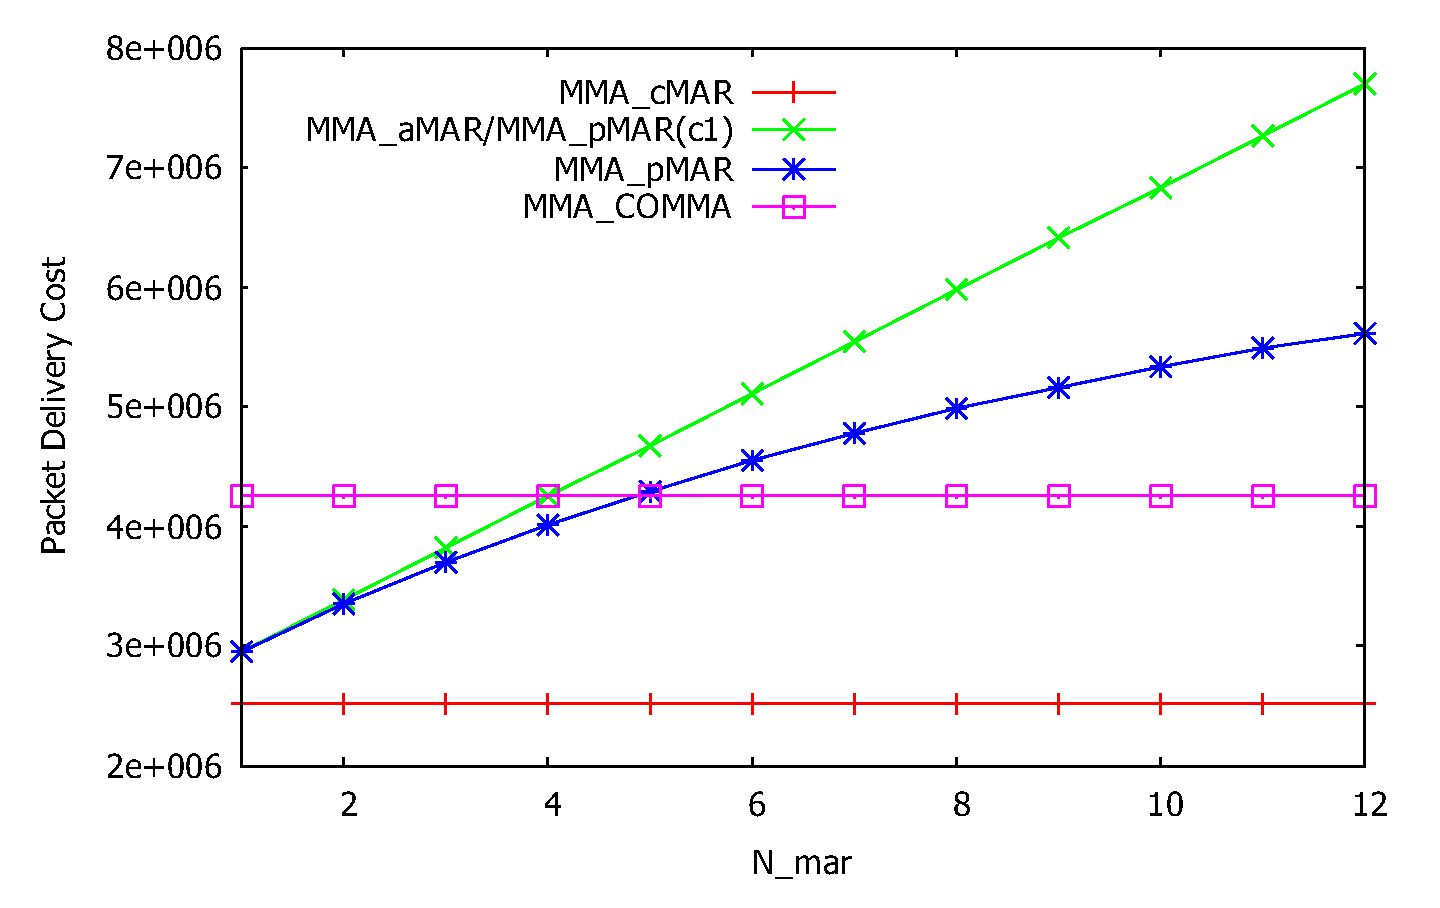
\includegraphics[width=0.50\textwidth]{./Part3/Chapter8/figures/c10_pc_n_mar.eps} \label{fig:c10_pc_n_mar}}
%\subfloat[]{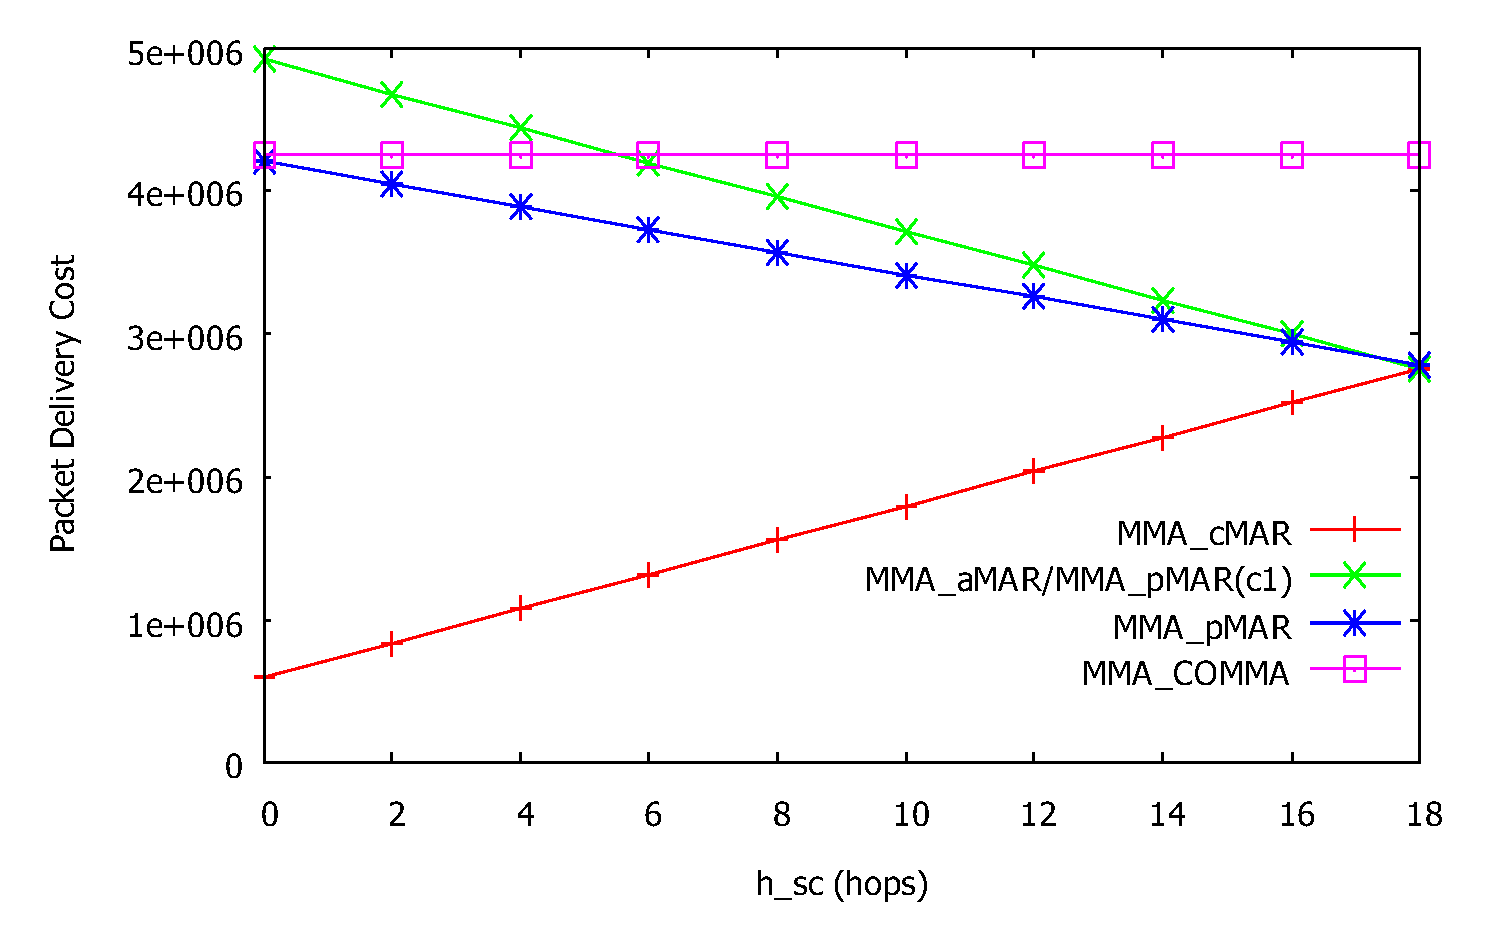
\includegraphics[width=0.50\textwidth]{./Part3/Chapter8/figures/c10_pc_h_sc.eps}\label{fig:c10_pc_h_sc}}
%\caption[Le coût de livraison de paquets.]{Le coût de livraison de paquets en termes de: (a) $N_{mar}$, (b) $h_{sc}$.}
%\label{fig:c10_pc}
%\end{figure}
%Similaire au délai de bout en bout, le coût de livraison de paquets (en fonction de $ N_{mar} $) en cas MMA\_cMAR et MMA\_COMMA est maintenu constant tandis que dans le cas MMA\_aMAR et MMA\_pMAR est fortement augmenté. La figure~\ref {fig:c10_pc_h_sc} montre le coût de livraison en fonction de $ h_{sc} $ quand $ h_{sa} + h_{sc} $ est fixé (18 sauts). Il apparaît clairement que le coût dans le cas MMA\_cMAR est nettement inférieur à celui dans les autres, même lorsque la source est très proche de l'aMAR. En outre, nous pouvons observer que ce coût en cas MMA\_pMAR (c1) est supérieur à celui de MMA\_pMAR en raison de multiples interfaces.
%\begin{figure}[h!]
% 	\begin{center} 
%		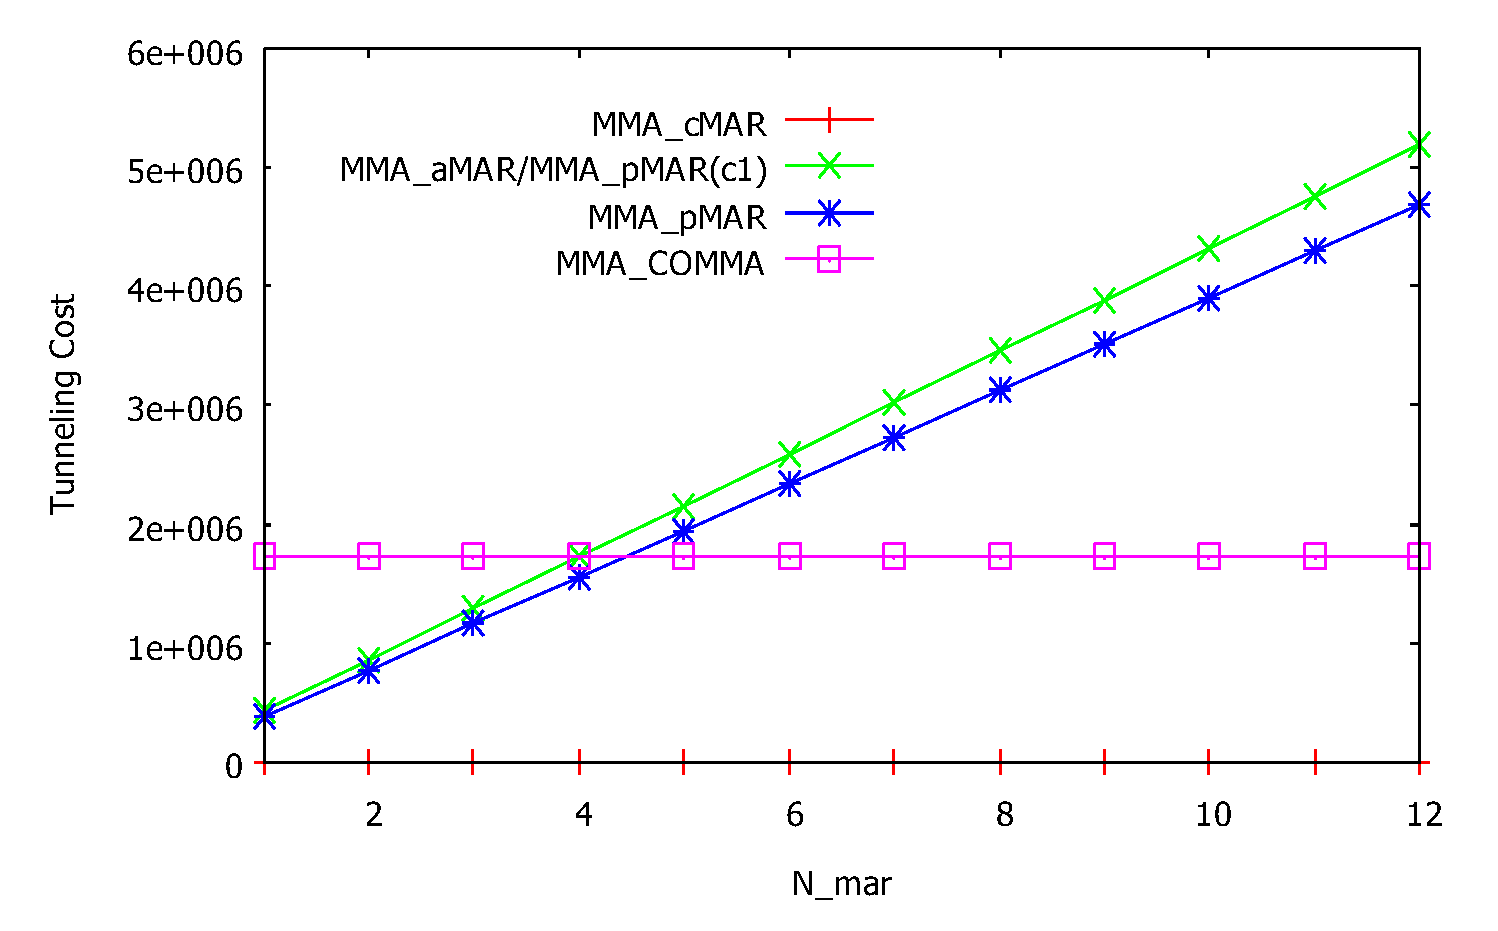
\includegraphics[width=0.50\textwidth]{./Part3/Chapter8/figures/c10_tc_n_mar.eps}
%		\caption[Le coût de tunnelisation.]{Le coût de tunnelisation comme une fonction de $N_{mar}$.}
%		\label{fig:c10_tc_n_mar}
%	\end{center}
%\end{figure}
%\paragraph{Le coût de tunnelisation}
%En ce qui concerne le coût de tunnelisation, la figure~\ref {fig:c10_tc_n_mar} montre le coût de tunnelisation en fonction de $ N_{mar} $. Le MMA\_cMAR n'introduit pas des surcharges de tunnel, alors que le coût de tunnelisation dans le MMA\_COMMA est fixé. D'autre part, il est significativement augmenté quand $ N_{mar} $ augmente en cas MMA\_aMAR et MMA\_pMAR. Encore une fois, en appliquant les multiples interfaces, le coût de tunnelisation en cas MMA\_pMAR augmente légèrement.
%
%\subsubsection{Conclusion de la partie d'analyse quantitative}
%De l'analyse de la performance et des résultats numériques, nous concluons qu'aucune des approches est toujours meilleure que les autres. Par exemple, le MMA\_pMAR est généralement un bon choix lorsqu'on considère l'interruption de service. Le MMA\_cMAR, en revanche, est un choix préféré en ce qui concerne le délai de bout en bout. Les autres approches peuvent être les plus appropriées, cependant, dans une situation spécifique. L'analyse de performance donne aussi une idée de l'utilisation d'un MMA commun (COMMA) qui sert comme un point d'ancrage seule ​​pour le service multicast pour tous les nœuds dans le domaine, donc reflétant le déploiement PMIPv6. Bien que cette approche présente une performance acceptable, par exemple, quand $ N_{mar} $ et $ \psi $ sont petites, COMMA pose un goulot d'étranglement et un point de panne unique. COMMA n'est pas non plus un bon choix quand un contenu local est disponible. Par conséquent, la comparaison entre le MMA\_COMMA et le mode par défaut donne l'idée de la performance de DMM en ce qui concerne PMIPv6 concernant le service multicast.
%
%Essentiellement, la performance des méthodes dépend de différents facteurs tels que le nombre de handovers ($ N_{mar} $, qui peut être considérée comme une fonction de la vitesse et du rayon de sous-réseau), l'échelle de réseau ($ \psi $), la position de la source ($h_{sc} $, $ h_{sa} $) et la densité de l'auditeur ($ h_{mi} $). Ce sont les raisons pour lesquelles un MMA fixe n'est pas une bonne stratégie. En outre, les utilisateurs mobiles quotidiens consacrent jusqu'à 62 \% de leur temps à la maison et au travail (en général, l'emplacement typique) \cite{cisco_connected_lives}. Ainsi, dans certains cas, l'emplacement typique serait également un bon candidat. Même les ancres de mobilité sont distribuées, certaines d'entre elles sont surchargées plus que les autres \cite{anchor_selection}. En conséquence, un support par flux de multicast doit être fourni.
%
%\subsection{La sélection dynamique de l'ancre multicast} \label{c10:dmma}
%Dans ce paragraphe, un mécanisme de sélection dynamique de l'ancre de mobilité multicast sera introduit. Sur la base des contextes collectés, le MMA sera sélectionné de façon dynamique afin de répondre à un ensemble des exigences. D'un point de vue du service, il contribue à satisfaire les exigences en termes de l'interruption de service et le délai, en particulier lorsqu'on considère des services en temps réel. Il fournit également un mécanisme permettant de mieux répartir la charge entre MARs. D'autres problèmes telles que la duplication de paquets et le laisser la latence (perte de ressources) peuvent être réduits. La sélection de MMA prend en compte non seulement le contexte de service multicast, mais aussi le contexte de la mobilité du nœud et le contexte de réseau, ainsi permettant une support multicast par flux. En d'autres termes, chaque flux multicast peut être traité différemment selon ​​differents contextes. La sélection de MMA peut être fait dynamiquement quand un flux est initié ou lorsque l'auditeur effectue un handover grâce au proxy MLD supportant plusieurs interfaces en amont.
%
%Pour sélectionner dynamiquement le MMA approprié, des contextes différents doivent être pris en compte comme le contexte de service multicast, le contexte de la mobilité du MN, et le contexte de réseau. Chaque contexte peut être affecté à un numéro de priorité. Par exemple, une valeur plus faible indique que le contexte est plus important. A ce stade, similaire au mode par défaut, quand un auditeur initie un flux multicast, le cMAR servira comme le MMA pour ce flux (le trafic multicast sera reçu directement à partir de l'infrastructure multicast). Cela signifie que la sélection MMA dans la phase initiale sera laissée pour les travaux au futur. Pour un flux de handover, le trafic multicast peut être reçu de l'aMAR, le pMAR, le cMAR, ou même un MAR dans lequel le canal multicast est déjà disponible, ou un MAR moins chargé afin de répondre à un ensemble des exigences. 
%
%Notre solution n'est pas seulement pour les problèmes de l'interruption de service et de délai de bout en bout, mais aussi pour autres problèmes liées au service multicast. Ainsi, elle peut offrir des avantages tels que :
%
%\begin{itemize}
%\item \textit{Une solution complète} pour la plupart des problèmes de l'auditeur liées à la mobilité (y compris l'interruption de service, le problème de convergence, le laisser de latence, le gaspillage des ressources, le routage sous-optimal et la perte de paquets);
%\item \textit{La route optimale} : Les flux multicast seront acheminés dans un mieux chemin, car ils ne passent pas toujours par leur ancre de mobilité.
%\item \textit{Evitant du problème de convergence du tunnel} : Cette solution peut résoudre complètement le problème de la convergence;
%\item \textit{L'utilisation dynamique de tunnel de mobilité} : L'utilisation de tunnel de la mobilité pour les sessions multicast en cours est activée dans les cas appropriés, par exemple, pour un contenu à distant, ou un canal avec des exigences de délai très strict;
%\item \textit{Gestion efficace du tunnel} : Dans un environnement DMM, il est impossible d'effectuer une pré-établir tous les tunnels entre MARs puisque le nombre de MARs est censé être grand. En permettant au proxy MLD avec multiples interfaces en amont, il peut causer la gestion complexe de tunnel (par exemple, l'entretien et la vie du tunnel). Ainsi, la solution proposée, qui est basée sur le module de gestion de la mobilité multicast, peut aider à résoudre ce problème;
%\item \textit{Répartition de la charge de flux multicast} : Puisque la sélection MMA prend la charge actuelle du MAR en compte, elle permet de meilleur répartir la charge de trafic multicast entre MARs.
%\item \textit{La gestion centralisée des canaux multicast} : L'entité centrale (Multicast Control Entity, ou MCE) recueille et gère les contextes considérés (par exemple, les canaux multicast et leur portée (locale ou distante)), améliorant le contrôle des fournisseurs de réseau;
%\item \textit{Possibilité d'être appliquée à la mobilité de la source multicast};
%\item \textit{Compatibilité avec la mobilité unicast}.
%\end{itemize}
%
%\subsubsection{Les contextes considérés}
%\paragraph{Le contexte du service multicast}
%Lorsque les services sont sensibles à l'interruption ou à la perte de paquets, le temps d'interruption de service doit être minimisé. Par exemple, il devrait être inférieur à 300ms pour un service en temps réel, tandis que 500 ms pour un service normal \cite{interruption_requirements}. Pour le service sensible au délai de bout en bout, un long tunnel de mobilité ce qui peut entraîner un haut retard, doit être évité. La recommandation UIT-T G.114 \cite{itu-t} suggère que si le temps de transmission unidirectionnelle de connexion peut être maintenu en dessous de 150 ms, la plupart des applications connaîtront une interactivité transparente. En outre, les flux à longue durée peuvent effectuer de nombreuses handovers tandis que les flux à courte durée semblent être lancé et terminé au même MAR sans effectuer aucun handover.
%\paragraph{Le contexte du nœud mobile}
%Un nœud mobile à haute mobilité effectue souvent des handovers. Si le trafic multicast est toujours acheminé par aMAR, le temps de séjour plus long, le plus grave de l'impact sera. En outre, le nombre de points d'ancrage et de tunnels peut être augmenté. Au contraire, pour le nœud de faible mobilité, le MN devrait rester à un ou plusieurs MARs la plupart du temps.
%\paragraph{Le contexte du réseau}
%La sélection MMA peut également être basée sur plusieurs contextes de réseau tels que la charge actuelle de MAR, la proximité géographique du MAR au MN ainsi que la politique de canal multicast. Par exemple, lorsque la charge de MAR est élevée, il peut entraîner de retard et de perte de paquets si ce MAR est sélectionné comme un point d'ancrage multicast. Dans ce cas, le moins chargé MAR (entre MARs qu'ont l'état de transmission multicast pour ce canal) peut être un candidat potentiel. La raison est  que si le canal est déjà disponible au MAR sélectionné, le temps d'interruption peut être réduit au minimum (pas besoin de temps pour rejoindre le canal multicast). En outre, avec une augmentation négligeable de la charge, ce MAR peut transférer le trafic vers le cMAR \cite{developing_ip_multicast}.
%
%\subsubsection{La description de l'architecture de la solution proposée}
%Afin de collecter et gérer les contextes considérés, une entité de réseau, appelé MCE est introduite. Le MAR met régulièrement à jour le contexte de MN et la charge actuelle de MAR au MCE en utilisant une extension de PBU / PBA (ou une extension de messages Heartbeat \cite{heartbeat}). Le MCE gère également tous les canaux multicast dans le domaine. Le contexte de service peut être définie basé sur la classe de QoS.
%
%Résidant dans le MAR, le module de gestion de la mobilité (MUMO) prend la responsabilité de toutes les actions liées à la mobilité multicast. La structure de ce module est illustrée dans la figure~\ref{fig:multicast_module} et brièvement décrite comme suit :
%\begin{figure}[t!]
% 	\begin{center} 
%		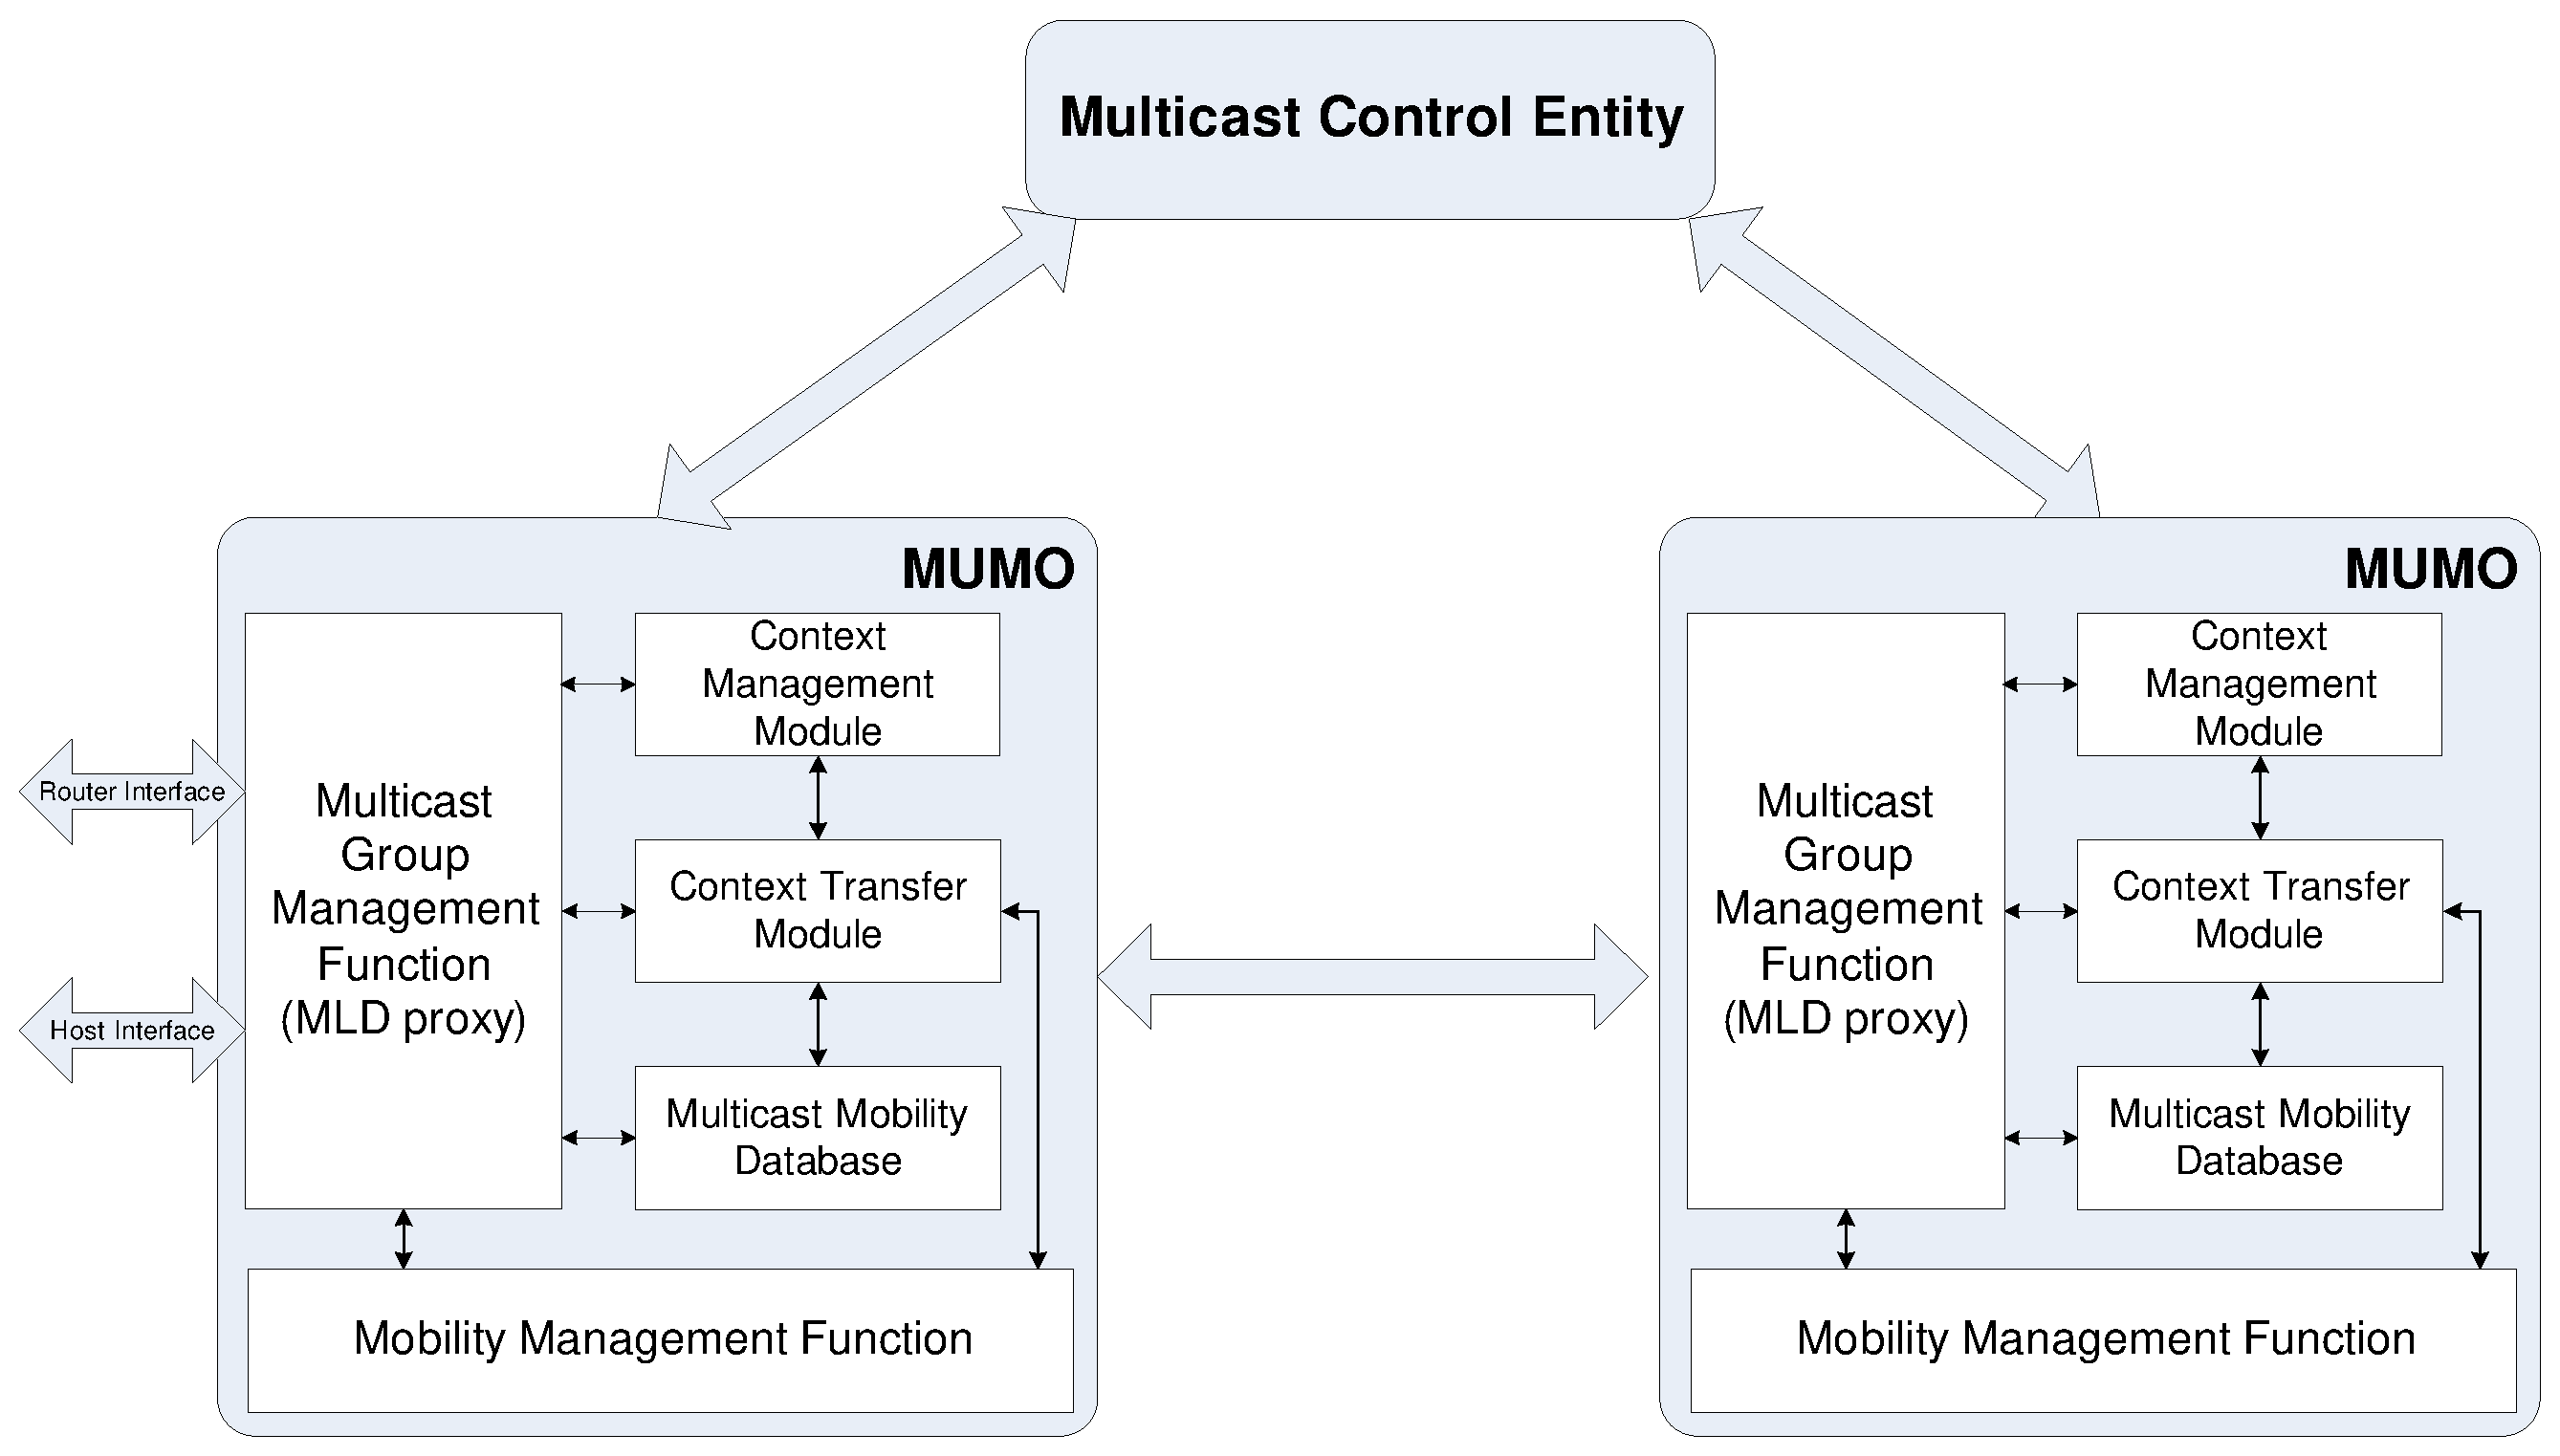
\includegraphics[width=0.80\textwidth]{./Part3/Chapter8/figures/c10_mume.eps}
%		\caption{Le module de gestion de la mobilité multicast (MUMO) à MAR.}
%		\label{fig:multicast_module}
%	\end{center}
%\end{figure}
%
%\setlength \abovedisplayskip{-1pt}
%\vspace{-0.1in}
%\begin{itemize}
%\itemsep 0.07em
%\item La fonction de gestion de groupe multicast (MGMF) réfère aux opérations de gestion de groupe et de stockage de l'information, qui est basée sur le proxy MLD avec plusieurs interfaces en amont\footnote{Ce module peut également être invoqué la fonction de routeur multicast par exemple, MRDv6.}. Ce module prend également en charge la fonction explicite de suivi afin de maintenir un état ​​du groupe de multicast par le client \cite{explicit_tracking}. Elle se fait sur ​​la base de Multicast Mobility Database (MMD), qui stocke les entrées avec les informations suivantes : i) l'identification de MN (MN\_ID); l'adresse de MN; et les abonnements des MNs. En outre, il maintient une structure de compteur pour le nombre d'auditeurs par canal multicast, ce qui permet d'identifier si un nœud est le dernier abonné du groupe.
%\item La fonction de gestion de contexte (CMF) communique avec le MCE pour récupérer les informations de configuration de canaux, y compris l'adresse de MMA correspondant, et le type de MMA (le précédent, l'ancrage, et le MAR courant ou autre). Basé sur cette information, le proxy MLD configure ses interfaces en amont vers les MARs correspondants.
%\item La fonction de transfert de contexte multicast (MCTF) est responsable d'échanger des informations d'abonnement multicast de MN entre MARs. Alors que le nouveau MAR peut rejoindre le flux courant à l'avance pour minimiser le temps d'interruption.
%\item La fonction de gestion de mobilité (MMF) ressemble à la pile de protocole de mobilité. Elle est responsable de l'attribution et le maintien de la connectivité IP d'un MN exécutant un handover à l'intérieur du domaine DMM. En d'autres termes, il est responsable de toutes les actions liées à la gestion de mobilité.
%\end{itemize}
%\begin{figure}[tb!] 
%  \begin{center} 
%    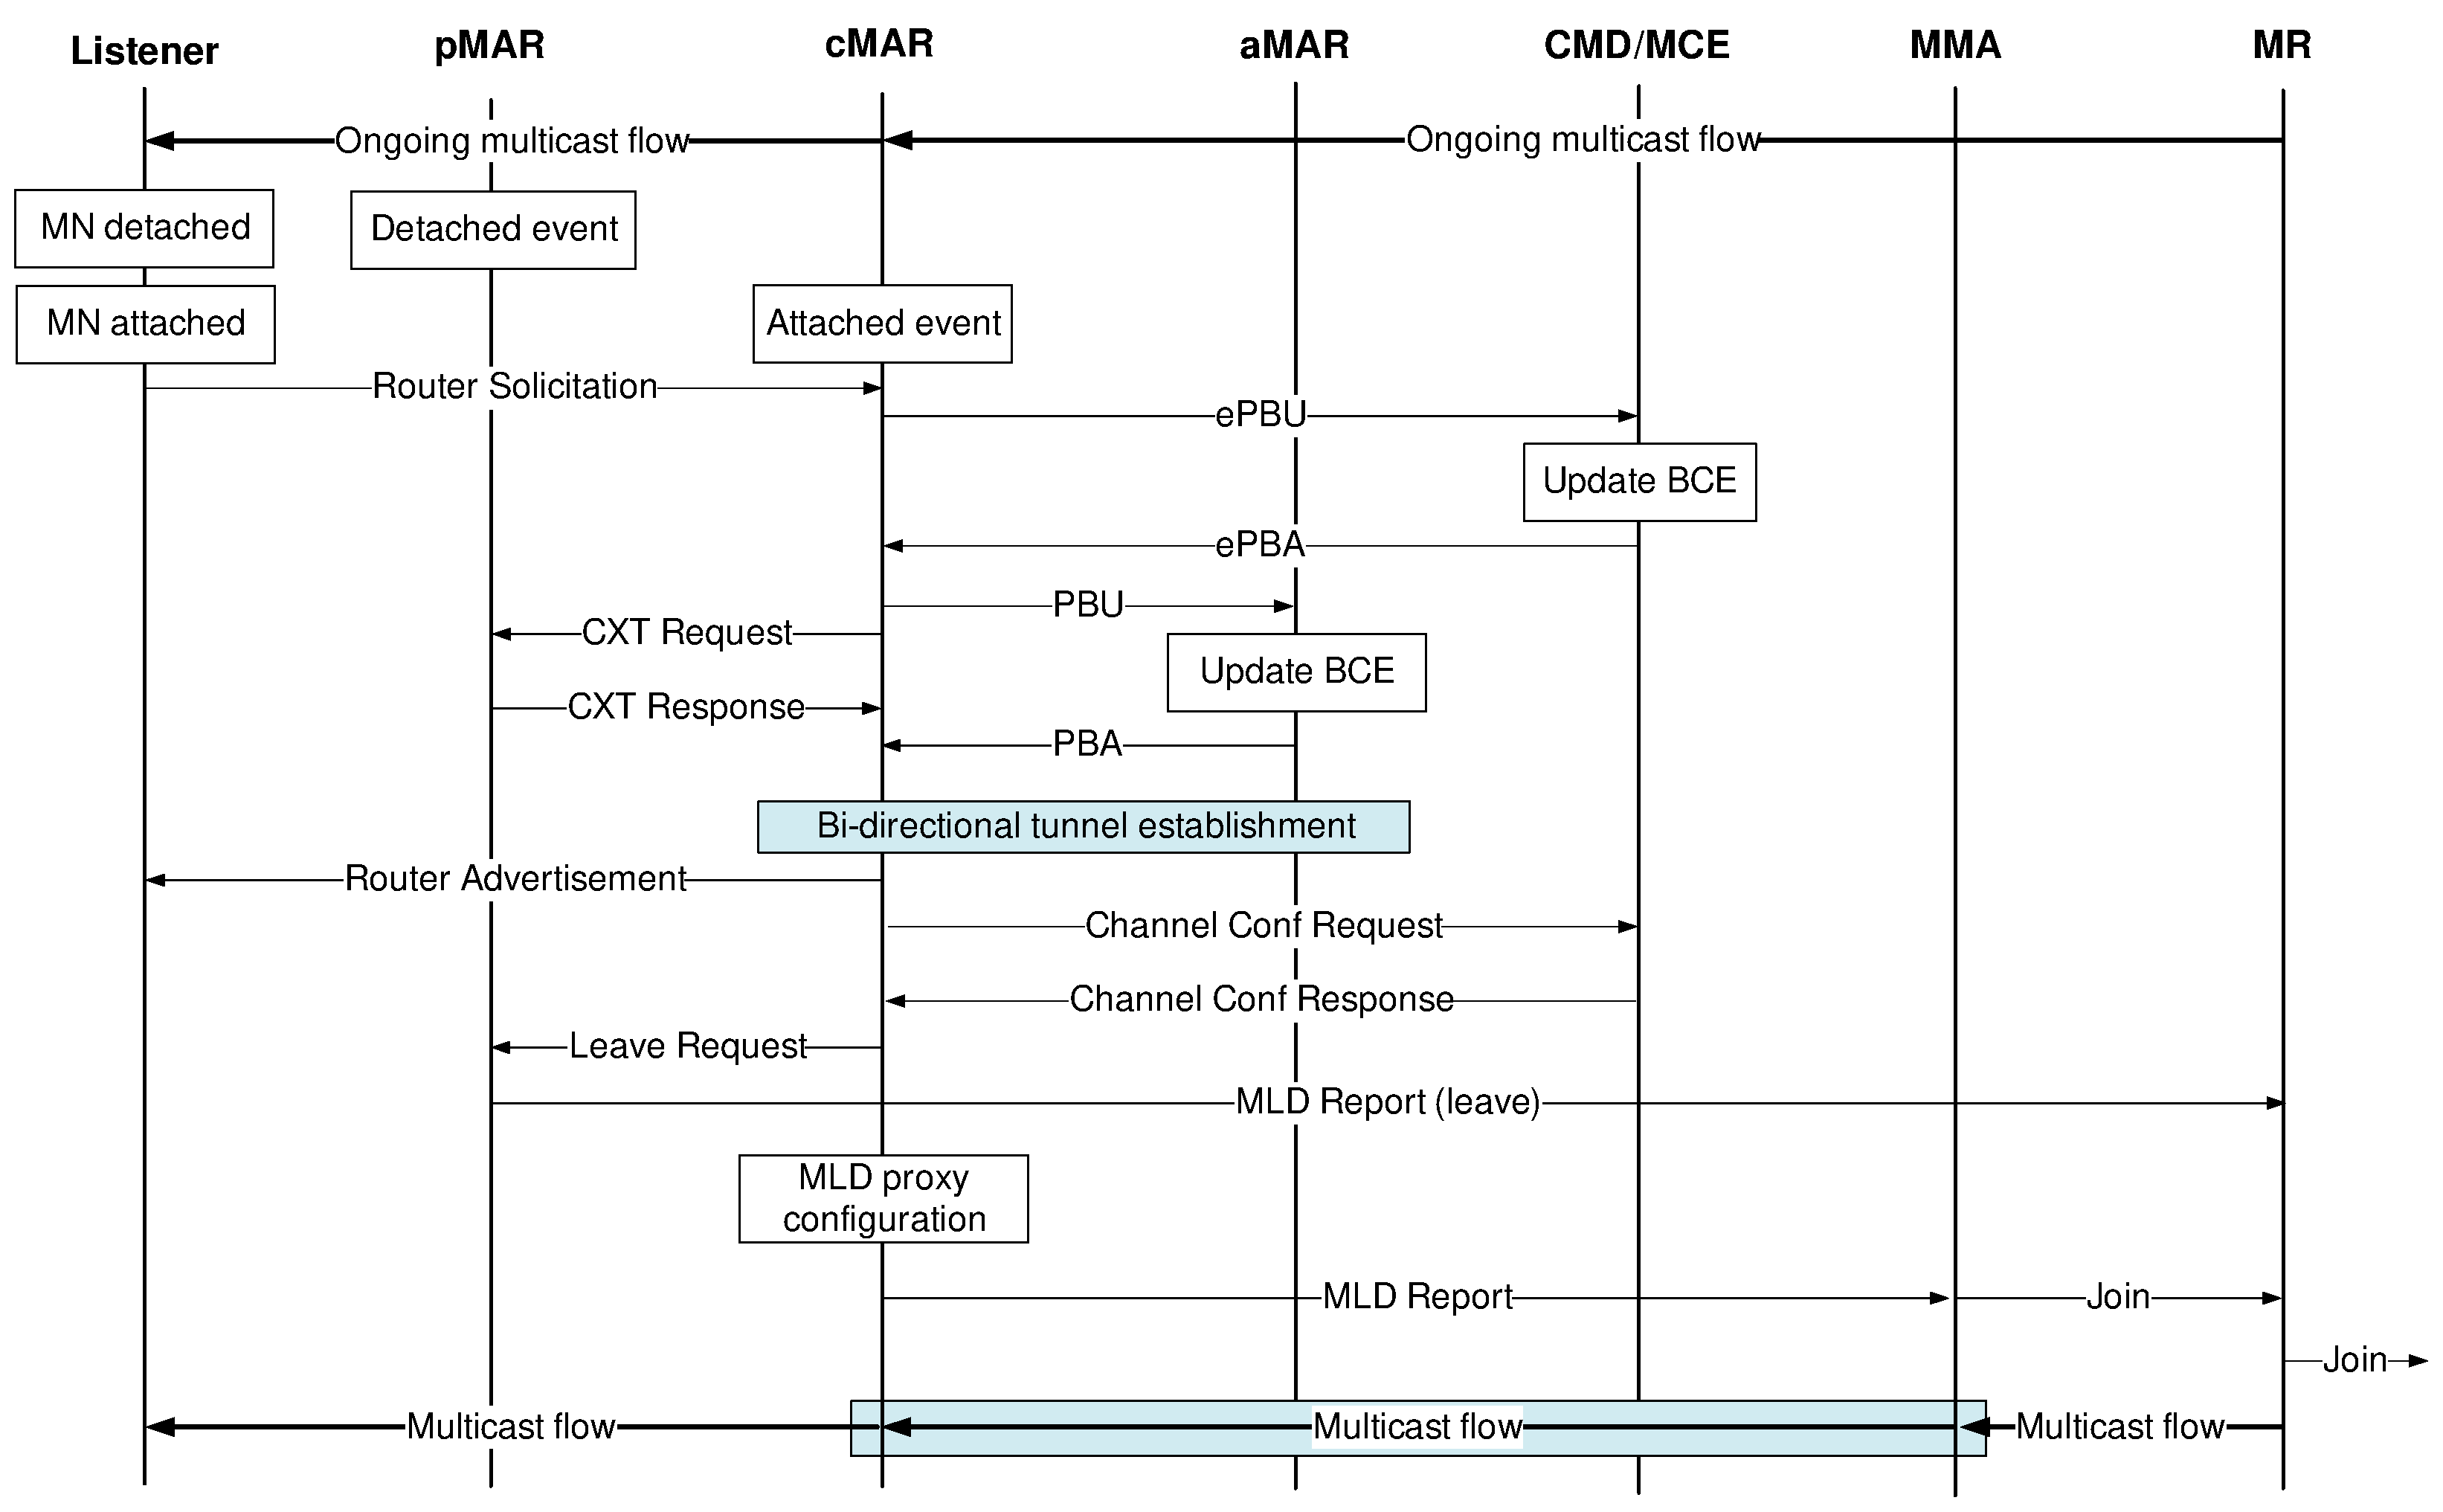
\includegraphics[width=0.85\textwidth]{./Part3/Chapter8/figures/c10_service_disruption_CXT_MMA.eps} 
%    \caption{La signalisation liée au service multicast avec la fonction de transfert de contexte multicast.}
%    \label{fig:c10_handover_signaling}
%  \end{center} 
%\end{figure}
%
%\subsubsection{Les opérations de la solution proposée}
%Les opérations de la solution sont brièvement présentées comme suit. Une fois que le MN entre dans un domaine de DMM (attache à MAR1), un préfixe est attribué à lui (dire Pref1). Le MAR1 envoie alors un message PBU y compris l'identification du MN (MN\_ID) et le Pref1 au CMD pour enregistrer ce MN. Après avoir reçu le PBU, le CMD crée une BCE qui se compose du MN\_ID, le Pref1, et l'adresse de MAR1 (comme aMAR) pour ce MN. En réponse, le message PBA est envoyé de CMD à MAR1 pour informer que l'emplacement de MN est mis à jour. Le MAR1 envoie un message RA y compris le Pref1 au MN. Le MN, après avoir configuré son adresse IPv6, peut adhérer à un flux multicast via le MAR courant.
%
%En cas de handover (voir figure ~\ref{fig:c10_handover_signaling}), le cMAR alloue un nouveau préfixe pour ce MN (appelé Pref2). Le cMAR envoie alors un PBU au CMD pour le nouveau enregistrement de préfixe. Ce message comprend le MN\_ID, et le Pref2. En regardant le tableau BCE, le CMD met à jour l'entrée correspondante au MN\_ID à l'emplacement actuel du MN. Le CMD répond alors par un message PBA, y compris la liste des adresses des points d'ancrage, les préfixes correspondants, et l'adresse du MAR précédent. À la réception de ce message, le cMAR échange les messages PBU/PBA avec MARs d'ancrage pour mettre à jour l'emplacement actuel du MN. Ainsi, le tunnel bidirectionnel est établi entre le cMAR et l'aMAR, si nécessaire. Le cMAR envoie alors un message RA, y compris le nouveau préfixe alloué au MN. Le MN peut donc configurer son adresse IPv6 et commencer une nouvelle communication avec le CN. En parallèle, les messages de transfert de contexte multicast sont échangés entre le cMAR et le pMAR permettant le cMAR d'obtenir les flux multicast en cours. Basé sur ces informations, le cMAR contacts avec le MCE pour obtenir les configurations de canaux qui composent les informations suivantes (par canal) : S, G, l'adresse de MMA, et un champ indiquant le rôle de MMA. Les messages PBU / PBA peuvent être étendus à transmettre la configuration de canal. Le cMAR configure une interface en amont vers le MMA, et envoie un rapport MLD au MMA pour rejoindre le canal multicast en cours. Après avoir rejoint l'arbre de transmission multicast (si nécessaire), le MMA transmet les paquets multicast au cMAR, et ils ont finalement atteint le MN. Si le cMAR ne reçoit pas le trafic multicast du pMAR, il demandera le pMAR pour arrêter la transmission du flux. Merci à la fonction explicite de suivi, le pMAR s'arrête la transmission du flux si le MN est le dernier membre de ce flux. Ainsi, il réduit le temps de latence et le gaspillage des ressources.
%
%\subsubsection{L'implémentation de la solution proposée}
%Une première version du DMMA était disponible grâce au projet Medieval \cite{d4.4, d6.4, ICC_Sergio}. Dans ce mode de réalisation, le module CMF exécute de façon simple : lorsque le MN agit comme un auditeur, le cMAR joue toujours le rôle du MMA. Au contraire, l'aMARs agit comme le MMA lorsque le MN joue le rôle d'une source. Cependant, les procédures pour l'acquisition des contextes considérés sont encore en cours de développement. Le module MMF est aussi en cours de développement basé sur la mise en œuvre de l'OAI PMIPv6. Les autres modules comme le MGMF et le MCTF sont déjà disponibles. Dans la prochaine étape, la mise en œuvre complète du module CMF sera déployée. Des expériences seront ensuite effectuées basé sur un banc d'essai proche d’un réseau réel.
%
%\vspace{-0.1in}
%\section{Conclusion et Perspectives}
%Le volume de données dans les réseaux mobiles est en plein essor principalement dû au succès des smartphones et des tablettes. Basé sur le fait que le trafic de l'Internet mobile sera dominé par la vidéo, l'évolutivité et l'efficacité de la bande passante de routage multicast permettent le multicast IP jouera un rôle plus important. Cependant, quand considérant le multicast IP dans un environnement mobile sans fil, il soulève plusieurs problèmes telles que l'interruptions de service, le délai de bout-en-bout, la duplication de paquets, le routage non-optimal et le gaspillage de ressources.
%
%Pour résoudre ces problèmes, cette thèse propose des solutions dans les environnements PMIPv6 et DMM. Grâce à cette thèse, les objectifs suivants sont atteints :
%\setlength \abovedisplayskip{-1pt}
%\vspace{-0.1in}
%\begin{itemize}
%\itemsep 0.07em
%\item \textit{Identifier les enjeux et les défis de la mobilité d'un nœud multicast et des métriques pour évaluer le mécanisme pour la mobilité d'un nœud multicast}
%\item \textit{Proposer une méthode expérimentale pour atteindre les résultats réalistes à faible coût} : La méthode expérimentale est proposé comme une combinaison des techniques de la virtualisation et de la simulation. Un banc d'essai PMIPv6 a été donc mis en œuvre.
%\item \textit{Présenter une méthode efficace pour optimiser la continuité de service en PMIPv6 et déployer un banc d'essai proche d’un réseau réel pour la mobilité d'un nœud multicast} : La solution proposée est basée sur le transfert de contexte multicast et la fonction de suivi explicite permettant au nouveau MAG pour obtenir les informations d'abonnement de MN à l'avance, ce qui réduit l'interruption de service.
%\item \textit{Proposer un mécanisme d'équilibrage de charge des flux multicast dans PMIPv6} : La solution proposée permet de mieux répartir la charge entre LMAs à améliorer l'évolutivité et la fiabilité du système.
%\item \textit{Introduire une solution pour le handover d'un nœud avec multiples interfaces dans des réseaux hétérogènes} : L'interface logique est utilisé en tant que la couche abstraite pour masquer le changement de l'interface physique de la pile IP. Merci à ce mécanisme, le MN n'est pas conscient de la mobilité du point de vue du service multicast. 
%\item \textit{Présenter un support à la mobilité inter-domaine pour les réseaux PMIPv6 et un support de base pour la mobilité de l'auditeur dans un environnement inter-domaine.}
%\item \textit{Proposer un mécanisme de sélection dynamique de l'ancre de mobilité multicast (DMMA) dans l'environnement  DMM}: Le DMMA non seulement supporte les services pour satisfaire l'exigence stricte en termes d'interruption et de délai de bout en bout, mais offre également des avantages tels que l'évitement du problème de la convergence, la gestion efficace du tunnel, le routage optimal, la réduction du gaspillage de ressources et la répartition de la charge.
%\end{itemize}
%
%\paragraph{Les bénéficie des solutions proposées}
%Une partie du mécanisme DMMA a été mis en œuvre dans le projet MÉDIÉVAL. Ce projet vise à fournir une architecture pour améliorer l'Internet mobile actuel et fournir des applications vidéo mobiles de manière plus efficace. Une solution multi-couche a été développée dans laquelle deux services typiques liés au multicast sont considérés comme le Mobile TV et le PBS. En ce qui concerne le support de la mobilité de nœud multicast, une solution à la fois pour l'auditeur et la source dans DMM a été fournie. Dans le cadre de la solution globale, le module de mobilité de multicast qui gère le soutien à la mobilité IP pour les flux multicast a été mis en œuvre. En plus d'informations, le transfert de contexte de multicast et la fonction explicite de suivi sont utilisés pour accélérer le processus d'acquisition de souscription du MN à réduire le temps d'interruption. Pour l'auditeur, le paquet multicast est toujours reçu directement de l'infrastructure multicast au MAR courant. Pour la source, le paquet multicast est acheminé à partir du MAR courant à celui d'ancrage par le tunnel de mobilité. 
%
%Dans le projet VELCRI, la solution pour un handover  sur ​​des réseaux hétérogènes est une partie du système de communication (y compris la communication véhicules-au-Grid et la communication Grid-aux-véhicules) pour fournir le service de charge pour le véhicule électrique. Le système de communication permet à l'EV à toujours être relié au Smart Grid en utilisant différentes technologies dans les différentes phases telles que LTE tout en conduisant, WLAN en approchant une station de recharge, et PLC tout en étant amarré à une station de recharge.\\ 
%Dans le projet SYSTUF, le DMMA sera utilisé pour fournir le service multicast pour les utilisateurs sur les transports publics, par exemple dans le tram et le métro. Dans plus de détails, le but du projet est de définir et de mettre en œuvre de nouveaux services à haut débit et un système de communication entre le sol et les véhicules en mouvement pour améliorer la qualité des transports urbains. Le DMMA sera étudié dans un scénario de forte mobilité.
%\paragraph{Perspectives}
%Avec la volonté de soutenir les services multicast IP dans un environnement mobile sans fil, cette thèse propose des solutions pour les problèmes liés à la mobilité d'un nœud multicast. Toutefois, puisqu'il y a plusieurs sujets définis, plusieurs aspects ne peuvent pas être analysés dans les détails, ce qui peuvent potentiellement être améliorés. Par exemple, alors que l'objectif de cette thèse a été jusqu'ici sur la mobilité de l'auditeur de multicast, la même idée peut être appliquée à la mobilité de la source. 
%
%Un autre sujet, qui serait considéré, est la mobilité du nœud. Autres modèles de mobilité seraient appliqués pour étudier l'impact de modèle de mobilité sur la performance de la solution. Il peut être fait en utilisant le modèle de mobilité existant dans NS-3.
%
%Comme la solution DMMA n'a été validée que par l'analyse mathématique, un banc d'essai DMM est en cours de déploiement. En outre, la prédiction de mobilité peut être utilisé pour améliorer la performance de DMMA qui permet de sélectionner le point d'ancre de mobilité de multicast adapté non seulement lors de l'exécution d'un handover, mais aussi au moment où le flux multicast est initié.
%
%L'intérêt croissant pour la technologie LTE par les opérateurs apporte le service Multicast/Broadcast Multimedia Service (MBMS) retour à l'ordre du jour pour soutenir l'augmentation exponentielle des services de distribution multimédia sur les réseaux cellulaires dans les prochaines années. Comme nous ne considérons pas la technologie d'accès sans fil spécifique, la mobilité d'un nœud multicast serait considéré dans l'architecture 3GPP.
% 
%A l'avenir, des milliards de véhicules seront connectés aux réseaux, qui créent de nouveaux défis et opportunités pour les opérateurs de réseau. Par conséquent, le mécanisme DMMA doit être envisagé, par exemple, pour les utilisateurs dans les véhicules à grande vitesse.
%
%Enfin, nous devons mettre notre solution dans la relation avec d'autres technologies comme le Software Defined Networking (SDN), l'Internet of Thing (IoT) et le Cloud Computing. Par exemple, la technique SDN peut changer le réseau de base  en permettant un déploiement distribué optimisé des instances virtualisées de passerelles mobiles. Cela pourrait faire beaucoup plus souple le façon de traiter les paquets et les flux IP. En outre, depuis les applications de IoT y compris l'ITS attirent de grand intérêt récemment, le support de la mobilité dans l'IoT aussi gagné beaucoup de l'élan. D'autre part, les avantages du Cloud Computing continuent de prendre de l'élan significatif. Comme les applications en cours d'exécution sur le Cloud ​​sont des médias riches, ou des applications de collaboration, le multicast IP peut offrir des avantages pour les utilisateurs, ainsi que pour les opérateurs \cite{cloud_multicast}. En outre, la répartition de l'infrastructure Cloud Computing entre les différents opérateurs de réseau influence également le scénario de développement de DMM \cite{cloud_dmm}.
